\chapter{Binary Neutron Star merger simulations} \label{ch:bns_sims}

%In this chapter we discuss the \ac{NR} \ac{BNS} merger simulations, 
%that were presented in related to this thesis publications 
%\citet{Nedora:2019jhl,Nedora:2020pak,Nedora:2021eoj}.
%%published in \citet{Nedora:2019jhl} and \citet{Nedora:2020pak}.
%%
%Simulations are performed with \ac{NR} code \wisky{}, that employs 
%methods discussed in the chapter~\ref{ch:nr_methods}. The specifics 
%of the numerical setup can be found in Appendix~\ref{app:whisky}.
%%
%We employ standard postprocessing techniques to extract the information 
%from simulations, \eg, mass-averaged quantities, that we discuss 
%detailed description of which can be found it Appendix~\ref{ch:ppr}.
%

%First 
%In Sec.~\ref{sec:bns_dynsmics_overview} we give the overview of the 
%\pmerg{} dynamics, expanding upon the general picture outlined in
%Sec.~\ref{sec:intro:merg_pmerg}. 
%In


%\subsubsection{TOV}

%To characterize these EOS, that employs very different microphyscis and 
%finite temperature properties and their relation to the electron fraction, we 
%consider the TOV solutions, presented on the figure \ref{fig:method:tov_mr}.
%The maximum mass of a non-rotating NS that these EOSs support are $2.06$, $2.06$, $2.42$ $None$ $None$ 
%for SFHo, LS220, DD2, BLh and SLy4 respectively. The NS radii, $R_{1.4}$, 
%then $11.9$, $12.7$, $13.2$ $\red{None}$ $\red{None}$, which in turn is related to 
%the pressure at half saturation density \cite{Lattimer:2012nd}. Thus we adopt the 
%following naming convention for EOS. Those that lead to a NS with smaller radii are 
%called "softer" and those that lead to a NS with larger radii are referred to as "stiffer" EOS.
%Among considered, the DD2 is the stiffest EOS, while SLy4 is the softest.




%% =====================================================================================
%%
%%               R E S U L T S
%%
%% =====================================================================================

\begin{figure*}[t]
    \centering 
    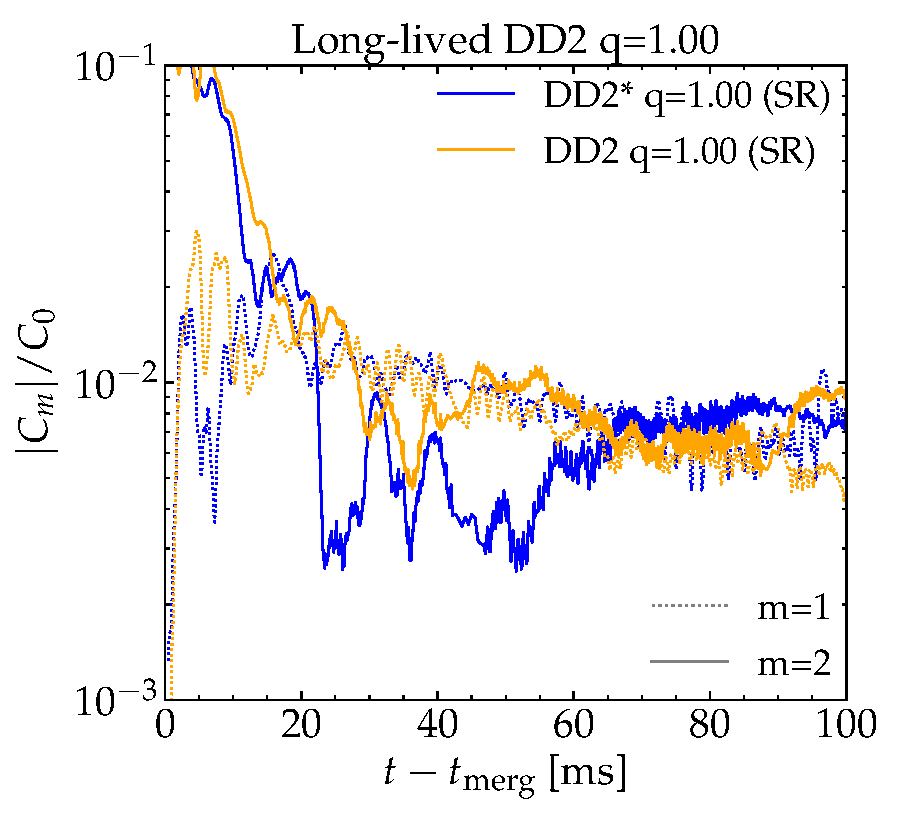
\includegraphics[width=0.49\textwidth]{remnant/dens_modes/modes_rho_dd2.pdf}
    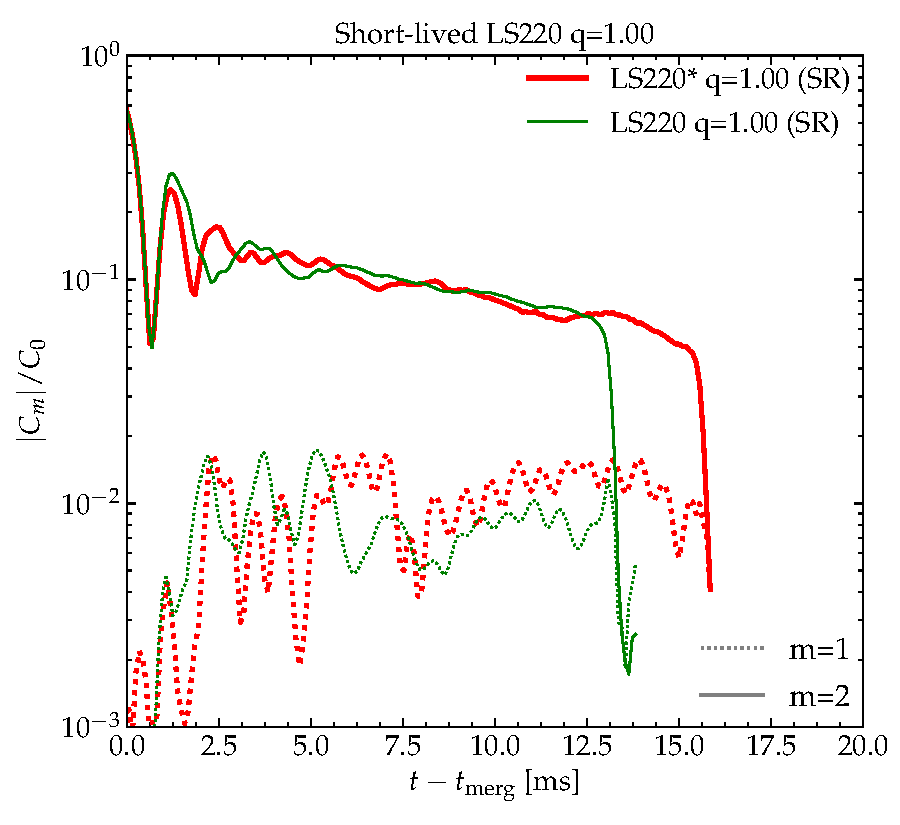
\includegraphics[width=0.49\textwidth]{remnant/dens_modes/modes_rho_ls220.pdf}
    \caption{
        The evolution of $m=1$ and $m=2$ modes in two representative 
        equal mass simulations with DD2 and LS220 \acp{EOS} on the 
        \textit{left panel} and the \textit{right panel} respectively. 
        %
        The mode amplitudes are computed via Eq.~\eqref{eq:modes}. 
        %
        The plot shows that the in the case of a long-lived remnant, 
        the $m=2$ mode is dumped, \ie, decays quickly after the merger, 
        and on a timescale of ${\gtrsim}20\,$ms it becomes comaprable to 
        $m=1$ mode. 
        %
        In case of a short-lived remnant, $m=2$ remains the dominant mode 
        until remnant collapses to a \ac{BH}.
        (Adopted from \cite{Nedora:2020pak}).
%        Modes analysis for exemplary equal-mass long-live and short-lived
%        remnants. The evolution of the $m=2$ and the $m=1$ monitored by
%        Eq.~\eqref{eq:modes} is shown for the DD2 and LS220 remnant with and
%        without turbulent viscosity. The $m=2$ mode in the long-lived
%        remnant is strongly damped by the emission of gravitational
%        radiation and becomes comparable to the $m=1$ mode on a timescale of
%        ${\gtrsim}20\,$ms. Turbulent viscosity sustain the $m=2$ mode for
%        a longer period. The $m=2$ mode is instead dominant to collapse in
%        the short-lived remnant.
%        (Adopted from \cite{Nedora:2020pak}).
    }
    \label{fig:dens_modes}
\end{figure*}


%\section{Results}


%\red{
%    To be defined: \\
%    Chirp pass \\
%    Gravitational and Baryonic masses
%}

%In this chapter we review the findings of \citet{Nedora:2019jhl} and \citet{Nedora:2020pak}
%and investigate the long-term \pmerg{} evolution of the binary neutron star. 
%
%Such studies are of high astrophysical importance as the ejecta of matter that occur 
%on various timescales \pmerg{} undergoes \rproc{} and produces observable EM emission. 
%The discussion of the \rproc{} and EM transits themselves, we resort for the chapter \red{chap:coutnerparts}.

In this chapter we preset the result of postprocessing of our 
\ac{BNS} merger simulations. 
For the discussion on simulation methods and postprocessing techniques, 
see Chapter \ref{ch:nr_methods}. 

We begin with discussing the dynamics of the \pmerg{} remnant, and 
its interaction with surrounding disk. Then we proceed with looking 
at the disk properties and their evolution in more details. Finally, we 
conclude the Sec.~\ref{sec:bns_sims:remdisk} by evaluating possible evolution 
trajectories beyond what was simulated. 
%
Next, in Sec.~\ref{sec:bns_sims:dyn} we analyze the properties of 
\ac{DE}, focusing on statistics, connecting them to the properties of the binary. 
Additionally, we investigate the origin and properties of the fast tail of 
\ac{DE} and \pmerg{} winds, connecting the latter to the remnant properties. 

The results presented in this Chapter are published in 
\citet{Nedora:2019jhl,Nedora:2020pak,Nedora:2020qtd,Nedora:2021eoj,Bernuzzi:2020txg}.


%% <<<< moved from EJECTA >>>> 



%\section{Simulations}\label{sec:bns_merg:sims}
%\subsection{Simulations}

%%% --------------------------------
%%% TAB SIM SUMMARY
%%\begin{table*}
\begin{sidewaystable}
\begin{center}
\captionsetup{width=1.0\linewidth}
    \caption{
      Summary table of all the simulations and dynamical ejecta properties. The columns contain
      the following information, starting from the left. Equation of
      state, mass-ratio, available resolutions,
      inclusion of subgrid turbulence, time of the
      simulation end, time of the BH formation for LR, SR, HR
      resolutions separately, time of last output, time the disk mass
      is extracted, disk mass, mass of the
      dynamical ejecta, mass-averaged electron fracton, terminal
      velocity and RMS angle (from the binary plane) for dynamical ejecta. For all
      data except $t_{BH}$, $t_{\text{end}}$ and $t_{\text{disk}}$, the value that is given is a mean value across resolutions, with an error estimated as one
      standard diviaion from the mean. In case where only one
      resolution is present, the error is assumed to be $20\%$ of the
      value. Adopted from \citet{Nedora:2020pak}.
    }
      %% \newtxt{For discussions on errors and convergence see \citep{Radice:2018pdn,Bernuzzi:2020txg}.
      %% The model data are available online at \citep{vsevolod_nedora_2020_4159619}.
%%       }
\scalebox{0.70}{
\begin{tabular}{c c c c c c c c c c c c c}
    \hline\hline
    EOS & $q$ & $\tilde{\Lambda}$ & Resolution & GRLES & $t_{\text{end}}$ & $t_{\text{BH}}$ & $t_{\text{disk}}$ & $M_{\text{disk}} ^{\text{last}}$ & $\md$ & $\langle \yd \rangle$ & $\langle \vd  \rangle$ & $\langle \theta_{\text{ej}} ^{\text{d}} \rangle$ \\
    &   &   &  &  & [ms] & [ms] & [ms] &   & $[10^{-2} M_{\odot}]$ &   & $[c]$ &   \\ 
    \hline
    \hline
    BLh & 1.00 & 541 & \texttt{LR SR HR} & \cmark & $43.3$ $91.8$ $23.1$ & $>43.3$ $>91.8$ $>23.1$ & 23.1 & $0.166^{+0.052} _{-0.052} $ & $0.14^{+0.02} _{-0.02} $ & $0.27^{+0.01} _{-0.01} $ & $0.17^{+0.01} _{-0.01} $ & $39.65^{+0.35} _{-0.35} $ \\
    BLh & 1.00 & 541 & \texttt{LR SR} & \xmark & $15.9$ $103.2$ $ $ & $>15.9$ $>103.2$ $ $ & 15.6 & $0.261^{+0.008} _{-0.008} $ & $0.12^{+0.01} _{-0.01} $ & $0.27^{+0.01} _{-0.01} $ & $0.16^{+0.01} _{-0.01} $ & $38.80^{+0.44} _{-0.44} $ \\
%%  BLh & 1.00 & 541 & \texttt{LR SR} & \xmark & $36.9$ $15.5$ $ $ & $>36.9$ $>15.5$ $ $ & 36.6 & $0.182^{+0.091} _{-0.091} $ & $0.21^{+0.04} _{-0.04} $ & $0.26^{+0.01} _{-0.01} $ & $0.18^{+0.01} _{-0.01} $ & $36.29^{+0.24} _{-0.24} $ \\
    \hline
    BLh & 1.18 & 539 & \texttt{LR} & \cmark & $69.4$ $ $ $ $ & $>69.4$ $ $ $ $ & 69.0 & $0.202^{+0.101} _{-0.101} $ & $0.30^{+0.06} _{-0.06} $ & $0.18^{+0.04} _{-0.04} $ & $0.19^{+0.04} _{-0.04} $ & $33.65^{+6.73} _{-6.73} $ \\
    BLh & 1.18 & 539 & \texttt{LR} & \xmark & $16.4$ $ $ $ $ & $>16.4$ $ $ $ $ & 15.9 & $0.229^{+0.115} _{-0.115} $ & $0.25^{+0.05} _{-0.05} $ & $0.16^{+0.03} _{-0.03} $ & $0.20^{+0.04} _{-0.04} $ & $30.86^{+6.17} _{-6.17} $ \\
    \hline
    BLh & 1.34 & 539 & \texttt{LR SR} & \cmark & $63.4$ $9.8$ $ $ & $>63.4$ $>9.8$ $ $ & 9.8 & $0.192^{+0.004} _{-0.004} $ & $0.25^{+0.05} _{-0.05} $ & $0.14^{+0.04} _{-0.04} $ & $0.17^{+0.00} _{-0.00} $ & $28.79^{+5.00} _{-5.00} $ \\
    BLh & 1.34 & 539 & \texttt{LR} & \xmark & $18.0$ $ $ $ $ & $>18.0$ $ $ $ $ & 18.0 & $0.211^{+0.106} _{-0.106} $ & $0.19^{+0.04} _{-0.04} $ & $0.17^{+0.03} _{-0.03} $ & $0.17^{+0.03} _{-0.03} $ & $33.39^{+6.68} _{-6.68} $ \\
    \hline
    BLh & 1.43 & 540 & \texttt{LR SR} & \cmark & $35.1$ $59.6$ $ $ & $>35.1$ $>59.6$ $ $ & 33.8 & $0.265^{+0.001} _{-0.001} $ & $0.27^{+0.08} _{-0.08} $ & $0.19^{+0.03} _{-0.03} $ & $0.16^{+0.00} _{-0.00} $ & $34.49^{+3.59} _{-3.59} $ \\
    \hline
    BLh & 1.54 & 543 & \texttt{LR} & \cmark & $45.8$ $ $ $ $ & $>45.8$ $ $ $ $ & 53.8 & $0.324^{+0.162} _{-0.162} $ & $0.20^{+0.04} _{-0.04} $ & $0.17^{+0.03} _{-0.03} $ & $0.13^{+0.03} _{-0.03} $ & $31.21^{+6.24} _{-6.24} $ \\
    BLh & 1.54 & 543 & \texttt{LR} & \xmark & $17.4$ $ $ $ $ & $>17.4$ $ $ $ $ & 30.1 & $0.287^{+0.144} _{-0.144} $ & $0.22^{+0.04} _{-0.04} $ & $0.21^{+0.04} _{-0.04} $ & $0.16^{+0.03} _{-0.03} $ & $35.05^{+7.01} _{-7.01} $ \\
    \hline
    BLh & 1.66 & 538 & \texttt{LR SR} & \cmark & $64.6$ $20.1$ $ $ & $>64.6$ $1.8$ $ $ & 19.2 & $0.289^{+0.005} _{-0.005} $ & $0.42^{+0.05} _{-0.05} $ & $0.11^{+0.01} _{-0.01} $ & $0.12^{+0.01} _{-0.01} $ & $24.08^{+0.29} _{-0.29} $ \\
    \hline
    BLh & 1.82 & 532 & \texttt{LR SR HR} & \cmark & $12.0$ $17.5$ $9.6$ & $1.4$ $1.4$ $1.5$ & 5.9 & $0.170^{+0.001} _{-0.001} $ & $0.81^{+0.04} _{-0.04} $ & $0.03^{+0.01} _{-0.01} $ & $0.11^{+0.00} _{-0.00} $ & $6.53^{+0.65} _{-0.65} $ \\
    BLh & 1.82 & 532 & \texttt{LR SR HR} & \xmark & $53.8$ $26.3$ $45.2$ & $1.7$ $1.3$ $1.0$ & 43.2 & $0.098^{+0.049} _{-0.049} $ & $1.07^{+0.07} _{-0.07} $ & $0.03^{+0.01} _{-0.01} $ & $0.12^{+0.00} _{-0.00} $ & $6.27^{+0.53} _{-0.53} $ \\
    \hline
    \hline
    DD2 & 1.00 & 853 & \texttt{LR SR}    & \xmark & $92.0$ $110.2$       & $>92.0$ $>110.2$        & 9.4 & $0.154^{+0.052} _{-0.052} $ & $0.11^{+0.01} _{-0.01} $ & $0.25^{+0.00} _{-0.00} $ & $0.18^{+0.01} _{-0.01} $ & $38.07^{+0.52} _{-0.52} $ \\
    DD2 & 1.00 & 853 & \texttt{LR SR HR} & \cmark & $123.0$ $113.0$ $74.4$ & $>123.0$ $>113.0$ $>74.4$ & 8.2 & $0.111^{+0.040} _{-0.040} $ & $0.12^{+0.03} _{-0.03} $ & $0.27^{+0.01} _{-0.01} $ & $0.16^{+0.00} _{-0.00} $ & $40.03^{+0.71} _{-0.71} $ \\
    \hline
    DD2 & 1.20 & 847 & \texttt{LR SR HR} & \xmark & $37.3$ $91.0$ $55.2$ & $>37.3$ $>91.0$ $>55.2$ & 36.6 & $0.261^{+0.028} _{-0.028} $ & $0.21^{+0.08} _{-0.08} $ & $0.18^{+0.03} _{-0.03} $ & $0.17^{+0.01} _{-0.01} $ & $29.07^{+3.75} _{-3.75} $ \\
    DD2 & 1.22 & 847 & \texttt{LR SR HR} & \cmark & $42.7$ $107.3$ $19.8$ & $>42.7$ $>107.3$ $>19.8$ & 8.7 & $0.209^{+0.033} _{-0.033} $ & $0.25^{+0.02} _{-0.02} $ & $0.19^{+0.01} _{-0.01} $ & $0.17^{+0.01} _{-0.01} $ & $30.74^{+0.89} _{-0.89} $ \\
    \hline
    DD2 & 1.43 & 820 & \texttt{LR SR} & \cmark & $37.7$ $62.0$ $ $ & $>37.7$ $>62.0$ $ $ & 36.7 & $0.304^{+0.051} _{-0.051} $ & $0.70^{+0.64} _{-0.64} $ & $0.14^{+0.05} _{-0.05} $ & $0.14^{+0.01} _{-0.01} $ & $25.51^{+9.58} _{-9.58} $ \\
    \hline
    \hline
    LS220 & 1.00 & 715 & \texttt{LR SR} & \cmark & $27.0$ $27.1$ $ $ & $13.7$ $13.7$ $ $ & 16.1 & $0.073^{+0.032} _{-0.032} $ & $0.16^{+0.02} _{-0.02} $ & $0.25^{+0.02} _{-0.02} $ & $0.16^{+0.01} _{-0.01} $ & $35.70^{+0.78} _{-0.78} $ \\
    LS220 & 1.00 & 715 & \texttt{LR SR HR} & \xmark & $35.9$ $37.2$ $27.1$ & $33.4$ $16.1$ $15.4$ & 34.6 & $0.072^{+0.006} _{-0.006} $ & $0.16^{+0.06} _{-0.06} $ & $0.22^{+0.00} _{-0.00} $ & $0.16^{+0.01} _{-0.01} $ & $34.99^{+1.68} _{-1.68} $ \\
    \hline
    LS220 & 1.05 & 715 & \texttt{SR HR} & \xmark & $ $ $23.3$ $24.1$ & $ $ $17.3$ $13.9$ & 22.3 & $0.107^{+0.054} _{-0.054} $ & $0.16^{+0.02} _{-0.02} $ & $0.21^{+0.01} _{-0.01} $ & $0.16^{+0.01} _{-0.01} $ & $33.28^{+2.37} _{-2.37} $ \\
    LS220 & 1.11 & 717 & \texttt{SR HR} & \xmark & $ $ $25.1$ $24.4$ & $ $ $17.0$ $>24.4$ & 24.2 & $0.140^{+0.071} _{-0.071} $ & $0.22^{+0.03} _{-0.03} $ & $0.19^{+0.02} _{-0.02} $ & $0.18^{+0.02} _{-0.02} $ & $30.25^{+4.43} _{-4.43} $ \\
    \hline
    LS220 & 1.16 & 714 & \texttt{SR HR} & \cmark & $ $ $95.8$ $11.3$ & $ $ $68.9$ $>11.3$ & 95.5 & $0.306^{+0.153} _{-0.153} $ & $0.34^{+0.00} _{-0.00} $ & $0.22^{+0.00} _{-0.00} $ & $0.16^{+0.00} _{-0.00} $ & $34.08^{+1.00} _{-1.00} $ \\
    LS220 & 1.16 & 714 & \texttt{LR SR HR} & \xmark & $29.5$ $36.1$ $28.8$ & $>29.5$ $>36.1$ $24.1$ & - & - & $0.33^{+0.05} _{-0.05} $ & $0.17^{+0.01} _{-0.01} $ & $0.17^{+0.01} _{-0.01} $ & $30.01^{+0.64} _{-0.64} $ \\
    \hline
    LS220 & 1.43 & 710 & \texttt{LR SR} & \cmark & $19.8$ $28.5$ $ $ & $15.7$ $12.3$ $ $ & 19.6 & $0.178^{+0.072} _{-0.072} $ & $0.73^{+0.03} _{-0.03} $ & $0.16^{+0.02} _{-0.02} $ & $0.17^{+0.01} _{-0.01} $ & $26.77^{+3.50} _{-3.50} $ \\
    \hline
    LS220 & 1.66 & 707 & \texttt{LR SR} & \cmark & $6.8$ $8.0$ $ $ & $1.4$ $2.1$ $ $ & 2.0 & $0.068^{+0.008} _{-0.008} $ & $1.11^{+0.38} _{-0.38} $ & $0.07^{+0.01} _{-0.01} $ & $0.14^{+0.01} _{-0.01} $ & $13.18^{+1.33} _{-1.33} $ \\
    \hline
    \hline
    SFHo & 1.00 & 413 & \texttt{SR HR} & \cmark & $ $ $25.3$ $11.6$ & $ $ $6.0$ $4.0$ & 50.0 & $0.023^{+0.012} _{-0.012} $ & $0.40^{+0.07} _{-0.07} $ & $0.21^{+0.00} _{-0.00} $ & $0.19^{+0.01} _{-0.01} $ & $32.48^{+1.79} _{-1.79} $ \\
    SFHo & 1.00 & 413 & \texttt{LR SR HR} & \xmark & $3.2$ $7.7$ $9.0$ & $>3.2$ $4.1$ $3.8$ & 7.2 & $0.019^{+0.007} _{-0.007} $ & $0.28^{+0.07} _{-0.07} $ & $0.23^{+0.01} _{-0.01} $ & $0.21^{+0.01} _{-0.01} $ & $31.66^{+1.80} _{-1.80} $ \\
    \hline
    SFHo & 1.13 & 412 & \texttt{SR HR} & \cmark & $ $ $14.2$ $14.3$ & $ $ $6.3$ $>14.3$ & - & - & $0.44^{+0.12} _{-0.12} $ & $0.18^{+0.01} _{-0.01} $ & $0.23^{+0.01} _{-0.01} $ & $33.20^{+0.78} _{-0.78} $ \\
    SFHo & 1.13 & 412 & \texttt{LR SR HR} & \xmark & $16.5$ $19.3$ $15.2$ & $5.5$ $11.6$ $3.9$ & 15.1 & $0.046^{+0.041} _{-0.041} $ & $0.42^{+0.03} _{-0.03} $ & $0.17^{+0.03} _{-0.03} $ & $0.22^{+0.01} _{-0.01} $ & $29.63^{+4.39} _{-4.39} $ \\
    \hline
    SFHo & 1.43 & 414 & \texttt{LR} & \cmark & $19.6$ $ $ $ $ & $4.8$ $ $ $ $ & 18.9 & $0.201^{+0.101} _{-0.101} $ & $0.38^{+0.08} _{-0.08} $ & $0.14^{+0.03} _{-0.03} $ & $0.20^{+0.04} _{-0.04} $ & $29.20^{+5.84} _{-5.84} $ \\
    SFHo & 1.43 & 414 & \texttt{SR} & \cmark & $ $ $46.5$ $ $ & $ $ $>46.5$ $ $ & 50.8 & $0.241^{+0.121} _{-0.121} $ & $0.24^{+0.05} _{-0.05} $ & $0.19^{+0.04} _{-0.04} $ & $0.14^{+0.03} _{-0.03} $ & $32.86^{+6.57} _{-6.57} $ \\
    \hline
    SFHo & 1.66 & 408 & \texttt{LR SR} & \cmark & $11.2$ $16.8$ $ $ & $1.3$ $1.3$ $ $ & 11.6 & $0.177^{+0.153} _{-0.153} $ & $0.15^{+0.00} _{-0.00} $ & $0.07^{+0.00} _{-0.00} $ & $0.12^{+0.01} _{-0.01} $ & $10.39^{+1.14} _{-1.14} $ \\
    \hline
    \hline
    SLy4 & 1.00 & 402 & \texttt{LR SR} & \cmark & $10.5$ $13.1$ $ $ & $2.8$ $2.8$ $ $ & - & - & $0.09^{+0.02} _{-0.02} $ & $0.23^{+0.02} _{-0.02} $ & $0.27^{+0.02} _{-0.02} $ & $30.81^{+2.81} _{-2.81} $ \\
    SLy4 & 1.00 & 402 & \texttt{LR SR} & \xmark & $12.7$ $22.0$ $ $ & $2.7$ $13.8$ $ $ & 12.5 & $0.071^{+0.175} _{-0.175} $ & $0.31^{+0.20} _{-0.20} $ & $0.23^{+0.03} _{-0.03} $ & $0.22^{+0.01} _{-0.01} $ & $32.23^{+4.84} _{-4.84} $ \\
    \hline
    SLy4 & 1.13 & 402 & \texttt{LR SR} & \xmark & $8.4$ $20.3$ $ $ & $>8.4$ $13.0$ $ $ & 8.0 & $0.164^{+0.023} _{-0.023} $ & $0.59^{+0.07} _{-0.07} $ & $0.16^{+0.00} _{-0.00} $ & $0.24^{+0.01} _{-0.01} $ & $29.67^{+1.97} _{-1.97} $ \\
    \hline
    SLy4 & 1.43 & 399 & \texttt{SR} & \cmark & $ $ $40.3$ $ $ & $ $ $>40.3$ $ $ & 45.2 & $0.200^{+0.100} _{-0.100} $ & $0.20^{+0.04} _{-0.04} $ & $0.21^{+0.04} _{-0.04} $ & $0.15^{+0.03} _{-0.03} $ & $34.03^{+6.81} _{-6.81} $ \\
    \hline
    SLy4 & 1.66 & 397 & \texttt{SR} & \cmark & $ $ $7.2$ $ $ & $ $ $1.2$ $ $ & 3.9 & $0.138^{+0.069} _{-0.069} $ & $0.28^{+0.06} _{-0.06} $ & $0.05^{+0.01} _{-0.01} $ & $0.12^{+0.02} _{-0.02} $ & $8.43^{+1.69} _{-1.69} $ \\
    \hline\hline
\end{tabular}
\label{tab:sim}
}%scalebox
\end{center}
%\end{table*}
\end{sidewaystable}



%\usepackage{lipsum}% dummy text
%\begin{document}
    %\lipsum % Text before
%    \afterpage{%
%        \clearpage% Flush earlier floats (otherwise order might not be correct)
%        \thispagestyle{empty}% empty page style (?)
%        \begin{landscape}% Landscape page
%            \centering % Center table
%            \begin{tabular}{c c c c c c c c c c c c c}
%                \hline\hline
%                EOS & $q$ & $\tilde{\Lambda}$ & Resolution & GRLES & $t_{\text{end}}$ & $t_{\text{BH}}$ & $t_{\text{disk}}$ & $M_{\text{disk}} ^{\text{last}}$ & $\md$ & $\langle \yd \rangle$ & $\langle \vd  \rangle$ & $\langle \theta_{\text{ej}} ^{\text{d}} \rangle$ \\
%                &   &   &  &  & [ms] & [ms] & [ms] &   & $[10^{-2} M_{\odot}]$ &   & $[c]$ &   \\ 
%                \hline
%                \hline
%                BLh & 1.00 & 541 & \texttt{LR SR HR} & \cmark & $43.3$ $91.8$ $23.1$ & $>43.3$ $>91.8$ $>23.1$ & 23.1 & $0.166^{+0.052} _{-0.052} $ & $0.14^{+0.02} _{-0.02} $ & $0.27^{+0.01} _{-0.01} $ & $0.17^{+0.01} _{-0.01} $ & $39.65^{+0.35} _{-0.35} $ \\
%                BLh & 1.00 & 541 & \texttt{LR SR} & \xmark & $15.9$ $103.2$ $ $ & $>15.9$ $>103.2$ $ $ & 15.6 & $0.261^{+0.008} _{-0.008} $ & $0.12^{+0.01} _{-0.01} $ & $0.27^{+0.01} _{-0.01} $ & $0.16^{+0.01} _{-0.01} $ & $38.80^{+0.44} _{-0.44} $ \\
%                %%  BLh & 1.00 & 541 & \texttt{LR SR} & \xmark & $36.9$ $15.5$ $ $ & $>36.9$ $>15.5$ $ $ & 36.6 & $0.182^{+0.091} _{-0.091} $ & $0.21^{+0.04} _{-0.04} $ & $0.26^{+0.01} _{-0.01} $ & $0.18^{+0.01} _{-0.01} $ & $36.29^{+0.24} _{-0.24} $ \\
%                \hline
%                BLh & 1.18 & 539 & \texttt{LR} & \cmark & $69.4$ $ $ $ $ & $>69.4$ $ $ $ $ & 69.0 & $0.202^{+0.101} _{-0.101} $ & $0.30^{+0.06} _{-0.06} $ & $0.18^{+0.04} _{-0.04} $ & $0.19^{+0.04} _{-0.04} $ & $33.65^{+6.73} _{-6.73} $ \\
%                BLh & 1.18 & 539 & \texttt{LR} & \xmark & $16.4$ $ $ $ $ & $>16.4$ $ $ $ $ & 15.9 & $0.229^{+0.115} _{-0.115} $ & $0.25^{+0.05} _{-0.05} $ & $0.16^{+0.03} _{-0.03} $ & $0.20^{+0.04} _{-0.04} $ & $30.86^{+6.17} _{-6.17} $ \\
%                \hline
%                BLh & 1.34 & 539 & \texttt{LR SR} & \cmark & $63.4$ $9.8$ $ $ & $>63.4$ $>9.8$ $ $ & 9.8 & $0.192^{+0.004} _{-0.004} $ & $0.25^{+0.05} _{-0.05} $ & $0.14^{+0.04} _{-0.04} $ & $0.17^{+0.00} _{-0.00} $ & $28.79^{+5.00} _{-5.00} $ \\
%                BLh & 1.34 & 539 & \texttt{LR} & \xmark & $18.0$ $ $ $ $ & $>18.0$ $ $ $ $ & 18.0 & $0.211^{+0.106} _{-0.106} $ & $0.19^{+0.04} _{-0.04} $ & $0.17^{+0.03} _{-0.03} $ & $0.17^{+0.03} _{-0.03} $ & $33.39^{+6.68} _{-6.68} $ \\
%                \hline
%                BLh & 1.43 & 540 & \texttt{LR SR} & \cmark & $35.1$ $59.6$ $ $ & $>35.1$ $>59.6$ $ $ & 33.8 & $0.265^{+0.001} _{-0.001} $ & $0.27^{+0.08} _{-0.08} $ & $0.19^{+0.03} _{-0.03} $ & $0.16^{+0.00} _{-0.00} $ & $34.49^{+3.59} _{-3.59} $ \\
%                \hline
%                BLh & 1.54 & 543 & \texttt{LR} & \cmark & $45.8$ $ $ $ $ & $>45.8$ $ $ $ $ & 53.8 & $0.324^{+0.162} _{-0.162} $ & $0.20^{+0.04} _{-0.04} $ & $0.17^{+0.03} _{-0.03} $ & $0.13^{+0.03} _{-0.03} $ & $31.21^{+6.24} _{-6.24} $ \\
%                BLh & 1.54 & 543 & \texttt{LR} & \xmark & $17.4$ $ $ $ $ & $>17.4$ $ $ $ $ & 30.1 & $0.287^{+0.144} _{-0.144} $ & $0.22^{+0.04} _{-0.04} $ & $0.21^{+0.04} _{-0.04} $ & $0.16^{+0.03} _{-0.03} $ & $35.05^{+7.01} _{-7.01} $ \\
%                \hline
%                BLh & 1.66 & 538 & \texttt{LR SR} & \cmark & $64.6$ $20.1$ $ $ & $>64.6$ $1.8$ $ $ & 19.2 & $0.289^{+0.005} _{-0.005} $ & $0.42^{+0.05} _{-0.05} $ & $0.11^{+0.01} _{-0.01} $ & $0.12^{+0.01} _{-0.01} $ & $24.08^{+0.29} _{-0.29} $ \\
%                \hline
%                BLh & 1.82 & 532 & \texttt{LR SR HR} & \cmark & $12.0$ $17.5$ $9.6$ & $1.4$ $1.4$ $1.5$ & 5.9 & $0.170^{+0.001} _{-0.001} $ & $0.81^{+0.04} _{-0.04} $ & $0.03^{+0.01} _{-0.01} $ & $0.11^{+0.00} _{-0.00} $ & $6.53^{+0.65} _{-0.65} $ \\
%                BLh & 1.82 & 532 & \texttt{LR SR HR} & \xmark & $53.8$ $26.3$ $45.2$ & $1.7$ $1.3$ $1.0$ & 43.2 & $0.098^{+0.049} _{-0.049} $ & $1.07^{+0.07} _{-0.07} $ & $0.03^{+0.01} _{-0.01} $ & $0.12^{+0.00} _{-0.00} $ & $6.27^{+0.53} _{-0.53} $ \\
%                \hline
%                \hline
%                DD2 & 1.00 & 853 & \texttt{LR SR}    & \xmark & $92.0$ $110.2$       & $>92.0$ $>110.2$        & 9.4 & $0.154^{+0.052} _{-0.052} $ & $0.11^{+0.01} _{-0.01} $ & $0.25^{+0.00} _{-0.00} $ & $0.18^{+0.01} _{-0.01} $ & $38.07^{+0.52} _{-0.52} $ \\
%                DD2 & 1.00 & 853 & \texttt{LR SR HR} & \cmark & $123.0$ $113.0$ $74.4$ & $>123.0$ $>113.0$ $>74.4$ & 8.2 & $0.111^{+0.040} _{-0.040} $ & $0.12^{+0.03} _{-0.03} $ & $0.27^{+0.01} _{-0.01} $ & $0.16^{+0.00} _{-0.00} $ & $40.03^{+0.71} _{-0.71} $ \\
%                \hline
%                DD2 & 1.20 & 847 & \texttt{LR SR HR} & \xmark & $37.3$ $91.0$ $55.2$ & $>37.3$ $>91.0$ $>55.2$ & 36.6 & $0.261^{+0.028} _{-0.028} $ & $0.21^{+0.08} _{-0.08} $ & $0.18^{+0.03} _{-0.03} $ & $0.17^{+0.01} _{-0.01} $ & $29.07^{+3.75} _{-3.75} $ \\
%                DD2 & 1.22 & 847 & \texttt{LR SR HR} & \cmark & $42.7$ $107.3$ $19.8$ & $>42.7$ $>107.3$ $>19.8$ & 8.7 & $0.209^{+0.033} _{-0.033} $ & $0.25^{+0.02} _{-0.02} $ & $0.19^{+0.01} _{-0.01} $ & $0.17^{+0.01} _{-0.01} $ & $30.74^{+0.89} _{-0.89} $ \\
%                \hline
%                DD2 & 1.43 & 820 & \texttt{LR SR} & \cmark & $37.7$ $62.0$ $ $ & $>37.7$ $>62.0$ $ $ & 36.7 & $0.304^{+0.051} _{-0.051} $ & $0.70^{+0.64} _{-0.64} $ & $0.14^{+0.05} _{-0.05} $ & $0.14^{+0.01} _{-0.01} $ & $25.51^{+9.58} _{-9.58} $ \\
%                \hline
%                \hline
%                LS220 & 1.00 & 715 & \texttt{LR SR} & \cmark & $27.0$ $27.1$ $ $ & $13.7$ $13.7$ $ $ & 16.1 & $0.073^{+0.032} _{-0.032} $ & $0.16^{+0.02} _{-0.02} $ & $0.25^{+0.02} _{-0.02} $ & $0.16^{+0.01} _{-0.01} $ & $35.70^{+0.78} _{-0.78} $ \\
%                LS220 & 1.00 & 715 & \texttt{LR SR HR} & \xmark & $35.9$ $37.2$ $27.1$ & $33.4$ $16.1$ $15.4$ & 34.6 & $0.072^{+0.006} _{-0.006} $ & $0.16^{+0.06} _{-0.06} $ & $0.22^{+0.00} _{-0.00} $ & $0.16^{+0.01} _{-0.01} $ & $34.99^{+1.68} _{-1.68} $ \\
%                \hline
%                LS220 & 1.05 & 715 & \texttt{SR HR} & \xmark & $ $ $23.3$ $24.1$ & $ $ $17.3$ $13.9$ & 22.3 & $0.107^{+0.054} _{-0.054} $ & $0.16^{+0.02} _{-0.02} $ & $0.21^{+0.01} _{-0.01} $ & $0.16^{+0.01} _{-0.01} $ & $33.28^{+2.37} _{-2.37} $ \\
%                LS220 & 1.11 & 717 & \texttt{SR HR} & \xmark & $ $ $25.1$ $24.4$ & $ $ $17.0$ $>24.4$ & 24.2 & $0.140^{+0.071} _{-0.071} $ & $0.22^{+0.03} _{-0.03} $ & $0.19^{+0.02} _{-0.02} $ & $0.18^{+0.02} _{-0.02} $ & $30.25^{+4.43} _{-4.43} $ \\
%                \hline
%                LS220 & 1.16 & 714 & \texttt{SR HR} & \cmark & $ $ $95.8$ $11.3$ & $ $ $68.9$ $>11.3$ & 95.5 & $0.306^{+0.153} _{-0.153} $ & $0.34^{+0.00} _{-0.00} $ & $0.22^{+0.00} _{-0.00} $ & $0.16^{+0.00} _{-0.00} $ & $34.08^{+1.00} _{-1.00} $ \\
%                LS220 & 1.16 & 714 & \texttt{LR SR HR} & \xmark & $29.5$ $36.1$ $28.8$ & $>29.5$ $>36.1$ $24.1$ & - & - & $0.33^{+0.05} _{-0.05} $ & $0.17^{+0.01} _{-0.01} $ & $0.17^{+0.01} _{-0.01} $ & $30.01^{+0.64} _{-0.64} $ \\
%                \hline
%                LS220 & 1.43 & 710 & \texttt{LR SR} & \cmark & $19.8$ $28.5$ $ $ & $15.7$ $12.3$ $ $ & 19.6 & $0.178^{+0.072} _{-0.072} $ & $0.73^{+0.03} _{-0.03} $ & $0.16^{+0.02} _{-0.02} $ & $0.17^{+0.01} _{-0.01} $ & $26.77^{+3.50} _{-3.50} $ \\
%                \hline
%                LS220 & 1.66 & 707 & \texttt{LR SR} & \cmark & $6.8$ $8.0$ $ $ & $1.4$ $2.1$ $ $ & 2.0 & $0.068^{+0.008} _{-0.008} $ & $1.11^{+0.38} _{-0.38} $ & $0.07^{+0.01} _{-0.01} $ & $0.14^{+0.01} _{-0.01} $ & $13.18^{+1.33} _{-1.33} $ \\
%                \hline
%                \hline
%                SFHo & 1.00 & 413 & \texttt{SR HR} & \cmark & $ $ $25.3$ $11.6$ & $ $ $6.0$ $4.0$ & 50.0 & $0.023^{+0.012} _{-0.012} $ & $0.40^{+0.07} _{-0.07} $ & $0.21^{+0.00} _{-0.00} $ & $0.19^{+0.01} _{-0.01} $ & $32.48^{+1.79} _{-1.79} $ \\
%                SFHo & 1.00 & 413 & \texttt{LR SR HR} & \xmark & $3.2$ $7.7$ $9.0$ & $>3.2$ $4.1$ $3.8$ & 7.2 & $0.019^{+0.007} _{-0.007} $ & $0.28^{+0.07} _{-0.07} $ & $0.23^{+0.01} _{-0.01} $ & $0.21^{+0.01} _{-0.01} $ & $31.66^{+1.80} _{-1.80} $ \\
%                \hline
%                SFHo & 1.13 & 412 & \texttt{SR HR} & \cmark & $ $ $14.2$ $14.3$ & $ $ $6.3$ $>14.3$ & - & - & $0.44^{+0.12} _{-0.12} $ & $0.18^{+0.01} _{-0.01} $ & $0.23^{+0.01} _{-0.01} $ & $33.20^{+0.78} _{-0.78} $ \\
%                SFHo & 1.13 & 412 & \texttt{LR SR HR} & \xmark & $16.5$ $19.3$ $15.2$ & $5.5$ $11.6$ $3.9$ & 15.1 & $0.046^{+0.041} _{-0.041} $ & $0.42^{+0.03} _{-0.03} $ & $0.17^{+0.03} _{-0.03} $ & $0.22^{+0.01} _{-0.01} $ & $29.63^{+4.39} _{-4.39} $ \\
%                \hline
%                SFHo & 1.43 & 414 & \texttt{LR} & \cmark & $19.6$ $ $ $ $ & $4.8$ $ $ $ $ & 18.9 & $0.201^{+0.101} _{-0.101} $ & $0.38^{+0.08} _{-0.08} $ & $0.14^{+0.03} _{-0.03} $ & $0.20^{+0.04} _{-0.04} $ & $29.20^{+5.84} _{-5.84} $ \\
%                SFHo & 1.43 & 414 & \texttt{SR} & \cmark & $ $ $46.5$ $ $ & $ $ $>46.5$ $ $ & 50.8 & $0.241^{+0.121} _{-0.121} $ & $0.24^{+0.05} _{-0.05} $ & $0.19^{+0.04} _{-0.04} $ & $0.14^{+0.03} _{-0.03} $ & $32.86^{+6.57} _{-6.57} $ \\
%                \hline
%                SFHo & 1.66 & 408 & \texttt{LR SR} & \cmark & $11.2$ $16.8$ $ $ & $1.3$ $1.3$ $ $ & 11.6 & $0.177^{+0.153} _{-0.153} $ & $0.15^{+0.00} _{-0.00} $ & $0.07^{+0.00} _{-0.00} $ & $0.12^{+0.01} _{-0.01} $ & $10.39^{+1.14} _{-1.14} $ \\
%                \hline
%                \hline
%                SLy4 & 1.00 & 402 & \texttt{LR SR} & \cmark & $10.5$ $13.1$ $ $ & $2.8$ $2.8$ $ $ & - & - & $0.09^{+0.02} _{-0.02} $ & $0.23^{+0.02} _{-0.02} $ & $0.27^{+0.02} _{-0.02} $ & $30.81^{+2.81} _{-2.81} $ \\
%                SLy4 & 1.00 & 402 & \texttt{LR SR} & \xmark & $12.7$ $22.0$ $ $ & $2.7$ $13.8$ $ $ & 12.5 & $0.071^{+0.175} _{-0.175} $ & $0.31^{+0.20} _{-0.20} $ & $0.23^{+0.03} _{-0.03} $ & $0.22^{+0.01} _{-0.01} $ & $32.23^{+4.84} _{-4.84} $ \\
%                \hline
%                SLy4 & 1.13 & 402 & \texttt{LR SR} & \xmark & $8.4$ $20.3$ $ $ & $>8.4$ $13.0$ $ $ & 8.0 & $0.164^{+0.023} _{-0.023} $ & $0.59^{+0.07} _{-0.07} $ & $0.16^{+0.00} _{-0.00} $ & $0.24^{+0.01} _{-0.01} $ & $29.67^{+1.97} _{-1.97} $ \\
%                \hline
%                SLy4 & 1.43 & 399 & \texttt{SR} & \cmark & $ $ $40.3$ $ $ & $ $ $>40.3$ $ $ & 45.2 & $0.200^{+0.100} _{-0.100} $ & $0.20^{+0.04} _{-0.04} $ & $0.21^{+0.04} _{-0.04} $ & $0.15^{+0.03} _{-0.03} $ & $34.03^{+6.81} _{-6.81} $ \\
%                \hline
%                SLy4 & 1.66 & 397 & \texttt{SR} & \cmark & $ $ $7.2$ $ $ & $ $ $1.2$ $ $ & 3.9 & $0.138^{+0.069} _{-0.069} $ & $0.28^{+0.06} _{-0.06} $ & $0.05^{+0.01} _{-0.01} $ & $0.12^{+0.02} _{-0.02} $ & $8.43^{+1.69} _{-1.69} $ \\
%                \hline\hline
%            \end{tabular}
%            \captionof{table}{
%            Summary table of all the simulations and dynamical ejecta properties. The columns contain
%            the following information, starting from the left. Equation of
%            state, mass-ratio, available resolutions,
%            inclusion of subgrid turbulence, time of the
%            simulation end, time of the BH formation for LR, SR, HR
%            resolutions separately, time of last output, time the disk mass
%            is extracted, disk mass, mass of the
%            dynamical ejecta, mass-averaged electron fracton, terminal
%            velocity and RMS angle (from the binary plane) for dynamical ejecta. For all
%            data except $t_{BH}$, $t_{\text{end}}$ and $t_{\text{disk}}$, the value that is given is a mean value across resolutions, with an error estimated as one
%            standard diviaion from the mean. In case where only one
%            resolution is present, the error is assumed to be $20\%$ of the
%            value. Adopted from \citet{Nedora:2020pak}.
%        }% Add 'table' caption
%        \end{landscape}
%        \clearpage% Flush page
%    }
%    %\lipsum % Text after
%%\end{document}




























%%% --------------------------------
%
%
%In total we consider a sample of $37$ models of unique binaries with the 
%chirp mass $\mathcal{M}_c = 1.188\,\Msun$ that corresponds to the source of \GW{}.
%%
%The total gravitational mass covers the range $M\in[2.73, 2.88]\,\Msun$, while the 
%mas ration $q=M_A/M_B\in[1,1.8]$. 
%%
%We show the masses and radii of computed models as markers in 
%Fig.~\ref{fig:method:tov_mr} and summarize their main properties, 
%and the dynamical ejecta properties in Tab.~\ref{tab:sim}.
%%
%Most simulations are performed with at least two resolutions, 
%\texttt{LR} and \texttt{SR}. 
%$16$ binaries are also simulated at high resolution, \texttt{HR}.
%In total $76$ models are computed and analyzed.
%%
%Several binaries that resulted in a formation of a \ac{NS} remnant that does not collapse 
%to a \ac{BH} are evolved up to $100\,$ms \pmerg.
%%
%Most simulations include the effects of subgrid turbulence. 
%Those that are not are marked with ``*'' next to the equation of state name.
%%
%The naming convention for simulations is the following: 
%the equation of state name, the mass ratio, and the resolution, \eg, 
%the ``BLh* $q=1.00$ (\texttt{SR})" would refer to the simulation of the equal mass
%binary performed with BLh \ac{EOS}, without subgrid turbulence and at standard resolution. If resolution is not mentioned, \texttt{SR} is assumed.
%%\red{might be redundant}
%%% mass ratio binaries has been already presented in \cite{Bernuzzi:2020txg}.
%%% Together with our previous data these simulations form the largest
%%% sample of merger simulations with microphysics available to date
%%% \citep{Bernuzzi:2015opx,Radice:2016dwd,Radice:2016rys,Radice:2017lry,
%%%        Radice:2018xqa,Radice:2018pdn,Perego:2019adq,Endrizzi:2019trv,Bernuzzi:2020txg}.  



%% ----------------------------------------------------------------------
%%
%% O V E R V I E W  O F  T H E  M E R G E R  D Y N A M I C S
%%
%% ----------------------------------------------------------------------

%\subsection{Overview of the remnant dynamics}
%\section{Overview of the remnant dynamics}
%\label{sec:bns_dynsmics_overview}


%This section is based on the \cite{Nedora:2020pak}





%\subsection{Overview}

%A newly born \ac{NS} \pmerg{} remnant is not axisymmetric. In addition to driving the angular 
%momentum transport, it is a strong emitter of \acp{GW} at kiloHertz frequencies.
%In ${\sim}10-20\,$ms \pmerg{} \acp{GW} remove about two times the 
%amount of energy that was lost during the inspiral and merger \citep{Bernuzzi:2015opx}.
%%
%After that, the contribution of \acp{GW} to the system evolution, specifically to the 
%angular momentum loss, drops \citep{Radice:2018xqa}. The long-term evolution, $\mathcal{O}(100)\,$ms,
%of the remnant is driven primarily by viscous processes and weak interactions.
%%
%After the emission of \acp{GW} subsides, the \ac{NS} remnant still has an excess 
%in angular momentum and gravitational mass, with respect to the cold, 
%rigidly rotating equilibrium with the same baryoinc mass \citep{Radice:2018xqa}.
%%
%Subsequent evolution of the \ac{NS} remnant proceeds towards the axisymmetric configuration 
%close to the mass-shedding limit. 
%Depending on the lifetime of the \ac{NS} remnant we distinguish \textit{long-lived}
%and \textit{short-lived} remnants (See also \ref{sec:intro:remnant}).
%However, would a \ac{NS} remnant reach a stable state or collapse to a \ac{BH} depends on the 
%details of \pmerg{} conditions and on the temperature and composition effects.
%

%% -------------------------------------------------------------
%%
%% R E M N A N T  D I S K  I N T E R A C T I O N
%%
%% -------------------------------------------------------------

\section{Overview of the remnant-disk interactions}\label{sec:bns_sims:remdisk}
%\subsection{Remnant-disk interaction}\label{sec:bns_sims:remdisk}



We begin by analyzing the \pmerg{} dynamics of \ac{NS} remnants.
Hydrodynamic instabilities are monitored by a decomposition in Fourier modes,
$e^{-i m \phi}$, of the Eulerian rest-mass density on the equatorial plane 
(see Sec.~\ref{sec:bns_sims:method:modes} for more details).
%[see Eq.~(1) of \citep{Radice:2016gym}] and characterized by the
%development of a $m=2$ followed by a $m=1$ mode 
%\citep{East:2015vix,Paschalidis:2015mla,Radice:2016gym,Lehner:2016wjg,Bernuzzi:2013rza,Kastaun:2014fna}.
%
%We begin by analyzing the \pmerg{} dynamics of the \ac{NS} remnant. The standard 
%probe is employed here, namely the complex decomposition of the hydrodynamical modes
%(see Sec.~\ref{sec:bns_sims:method:modes}). 
%
We consider two representative simulations, 
LS220 $q=1.00$ (\texttt{SR}) %the model with LS220 \ac{EOS}, $q=1.00$ and a 
and 
DD2 $q=1.00$ (\texttt{SR}) 
that produce short- and long-lived remnants respectively.

%
As we mentioned in Sec.~\ref{sec:intro:merg_pmerg}, 
newly born \ac{NS} remnants are not axisymmetric, 
displaying characteristic spiral arms in their density 
profile that extend outwards from the shock interface of collided cores. 
%\citep{Shibata:1999wm,
%    Shibata:2006nm,Bernuzzi:2013rza,Kastaun:2014fna,East:2015vix,Paschalidis:2015mla,
%    Radice:2016gym,Lehner:2016wjg
%}.
%
%These arms, albet in terms of the angular momentum flux (defined in Sec.~\ref{sec:bns_sims:method:ang_mom}) can be seen in Fig.~\ref{fig:ang_mom_flux}. 
%

The result of the mode analysis is shown in Fig.~\ref{fig:dens_modes}. 
The $m=2$ instability, characterized by the bar-shaped geometry, dominates 
the early \pmerg{} while the $m=1$ instability, characterized by one-armed geometry,  
starts to dominate in the late evolution 
\citep[\eg][]{East:2015vix, %Paschalidis:2015mla,Radice:2016gym,Lehner:2016wjg,
    Bernuzzi:2013rza,Kastaun:2014fna}.
Fig.~\ref{fig:dens_modes} corroborates this picture.
%
%\red{One sentence 'why', physically}
%
Indeed, the $m=2$ mode remains the dominant one until 
${\sim}15-20\,$ms \pmerg{}. 
After that, the 
LS220 $q=1.00$ model 
%model with LS220 \ac{EOS} and $q=1.00$
forms a \ac{BH}. 
In the 
DD2 $q=1.00$ model, 
%model with DD2 \ac{EOS} and $q=1.00$ model, 
however, the amplitude of $m=1$ mode 
becomes comparable with that of $m=2$ and 
both modes persist throughout the remainder of the evolution,
after \ac{GW}-dominated phase ends 
%while 
%the $m=2$ mode efficiently dissipates through \ac{GW} emission 
\citep{Bernuzzi:2015opx,Radice:2016gym}. 
%
%\red{Why $m=1$ does not dissipates via \acp{GW}}
%
%Notably, the inclusion of subgrid turbulence sustains $m=1$ 
%on a longer timescale.
%
We find that the magnitude of the $m=1$ mode increases with the binary \mr{}.
For instance the largest $C_{m=1}$ are found in models with 
BLh and LS220 \acp{EOS} and \mr{}s $q=1.43$ and $q=1.22$ respectively. 
% Stronger $m=1$ leads to more large \ac{SWW} mass flux.  %------------------------------------------- ABOUT WIND
The dependency of the $C_{m=2}$ on \mr{} however is not very clear. 
Overall, our results are in agreement with what was 
reported by \citet{Lehner:2016wjg}.


\begin{figure}[t]
    \centering
    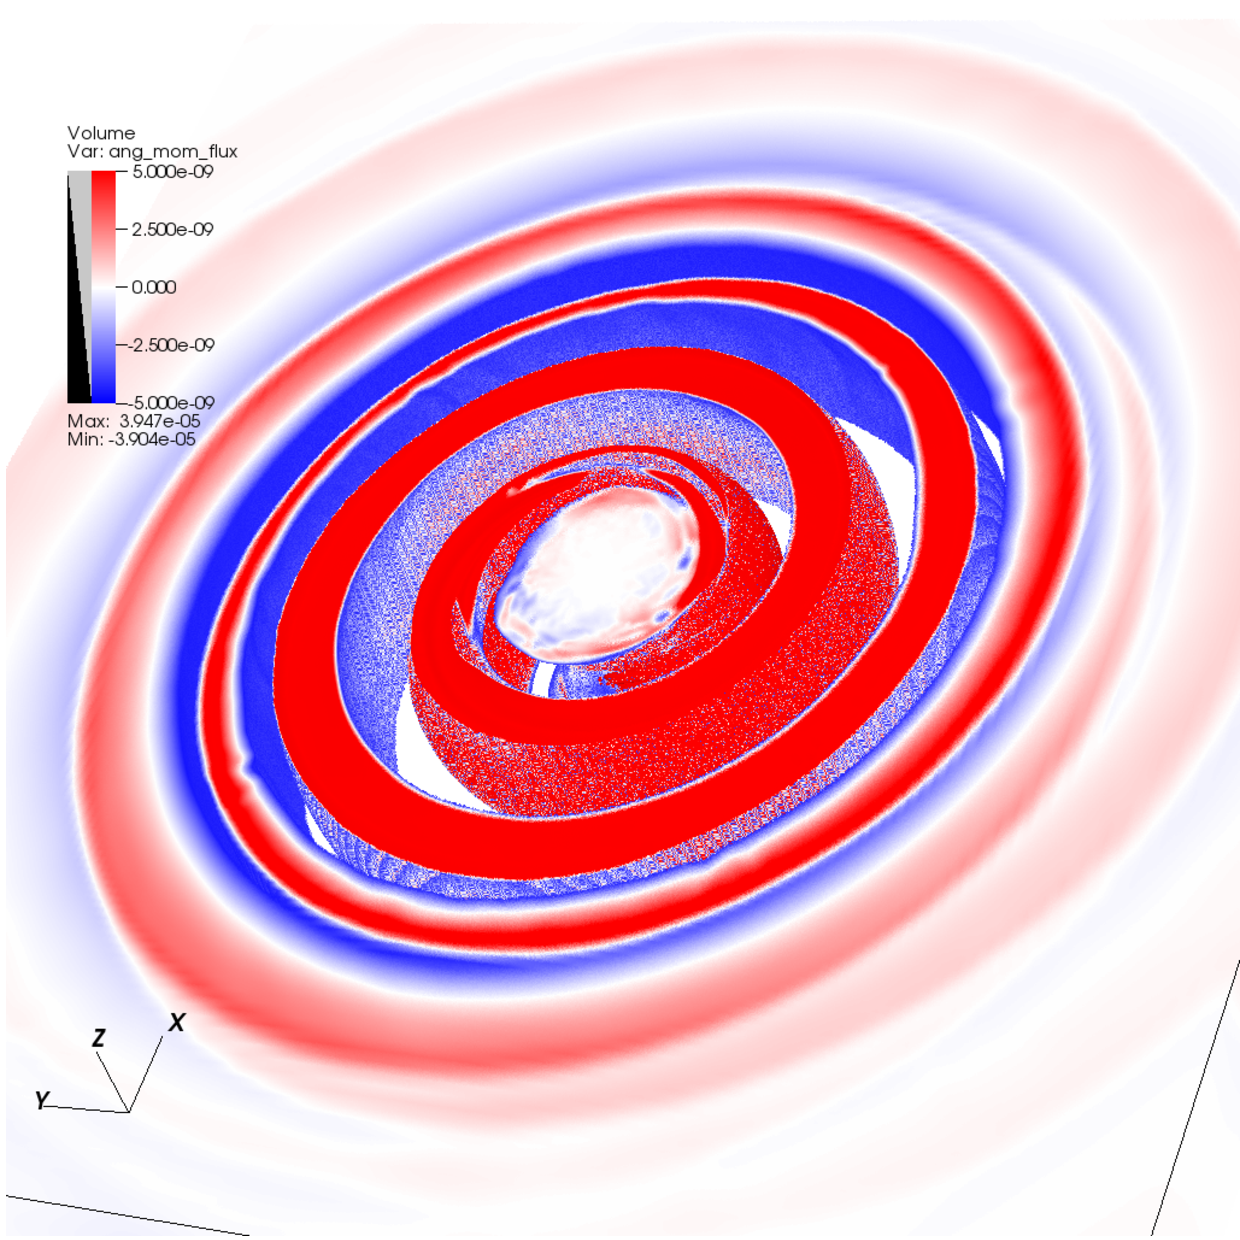
\includegraphics[width=0.49\textwidth]{raycasting_smooth_cropped.pdf}
    \caption{
        Volume rendering of the angular momentum flux, $J_r$, 
        distribution in $3D$ for DD2 $q=1.00$ \texttt{SR} model. 
        The snapshot is taken at ${\sim}43.5$~ms after
        merger. $J_r$ is shown on a central region of
        $(89\times89\times60)$~km${}^3$ covering the remnant NS
        and disk, and it is given in units where $c=G=\Msun=1$.
        (Adapted from \citet{Nedora:2019jhl}).
    }
    \label{fig:ang_mom_flux}
\end{figure}

\begin{figure}[t]
    \centering 
    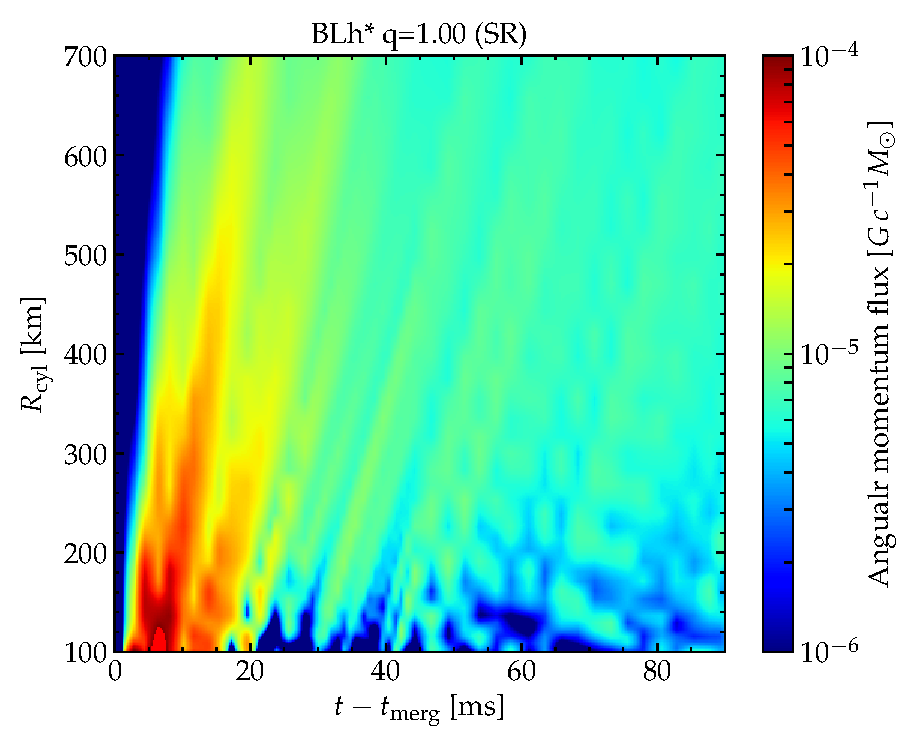
\includegraphics[width=0.49\textwidth]{remnant/evol_jflux_2d_BLh_M13651365_M0_SR_R1.pdf}
    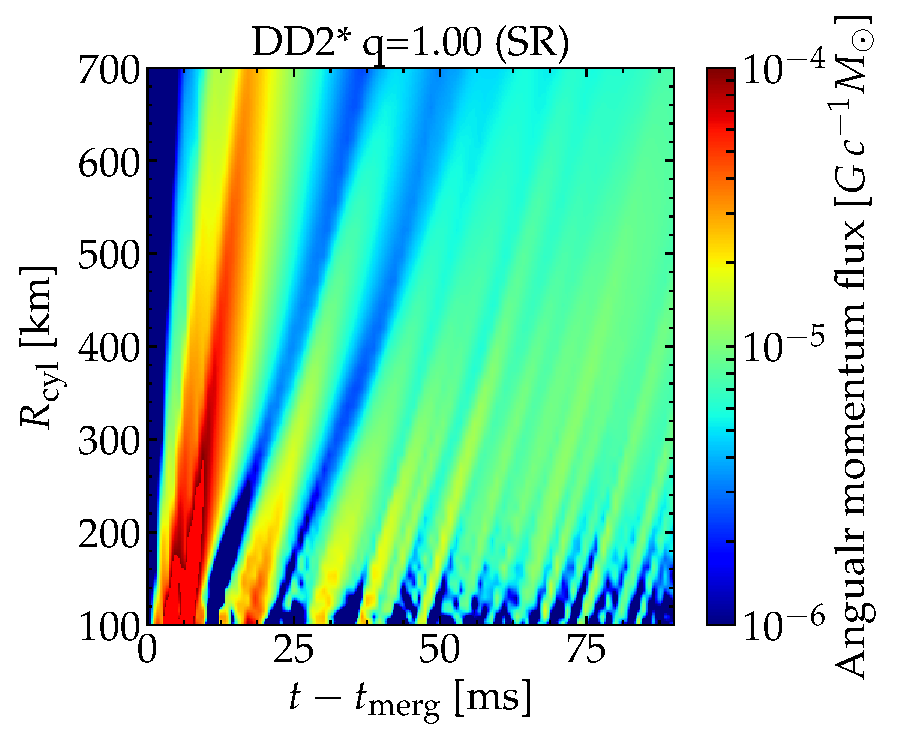
\includegraphics[width=0.49\textwidth]{remnant/evol_jflux_2d_DD2_M13641364_M0_SR_R1.pdf}
    \caption{
        The evolution of the angular momentum flux through consecutive cylindrical
        surfaces 
        (for cylindrical radii from $R_{\text{cyl}}=100$ to $R_{\text{cyl}}=500$). 
        The angular momentum transport through the disk is depicted 
        for two equal mass \ac{BNS} \pmerg{} remnants without viscosity.
        (Adapted from \citet{Nedora:2020pak}).
    }
    \label{fig:disk_ang_mom_flux_map_blh_q1}
\end{figure}


Formation of spiral arms is a generic hydrodynamic effect, 
that was identified in \ac{NR} simulations with polytropic 
\acp{EOS} \citep{Bernuzzi:2013rza,Radice:2016gym}.
However, evolution of these arms and quantitative behaviour of hydrodynamic
modes depend on the physics input of simulations, and are not well understood. 
We observe that turbulent viscosity, for instance, 
leads to faster suppression of the $m=2$. By contrast, the $m=1$ modes are not
significantly affected by viscosity, as shown in Fig.~\ref{fig:dens_modes}.
%
If a remnant is short-lived, as is the case for LS220 $q=1.00$ model, 
%with LS22 \ac{EOS} and $q=1.00$, 
the effect of subgrid turbulence is not apparent because 
the dynamical evolution is interrupted by the collapse.

%From the fluid's stress energy tensor,
%we compute the angular momentum density flux $J_r = T_{ra}(\p_\phi)^a$,
%where $\phi$ is the cylindrical angular coordinate;
%angular momentum is conserved if $(\p_\phi)^a$ is a Killing vector.
%
We compute the angular momentum and its flux from the energy-momentum 
tensor, Eq.~\eqref{eq:theory:tmunu_perf},
in cylindrical coordinates, $(r,\, \phi,\, z)$, under the additional
assumption of axisymmetry %with $(\partial_{\phi})^a$ being a Killing vector
(see Sec.~\ref{sec:bns_sims:method:ang_mom} for more details).
%
The disk is assumed to be comprised of matter with $\rho\leq10^{13}\,$\gcm{} 
(see also Sec.~\ref{sec:bns_sims:method:disk}).

We find that for a long-lived \ac{NS} remnant on a timescale of ${\sim}20$~ms, 
about half of the total angular momentum of the remnant is transferred 
into the disk. 
%% [ from shibata review ]
This is a consequence of the fact that the remnant \ac{NS} is strongly deformed 
after merger and exerts gravitational torques on the surrounding matter, 
that allow for a rapid angular momentum transport.
%% ---
%After, the remnant and the disk settle on quasi-stationary evolution path.
%(see Sec.~\ref{sec:bns_dynsmics_overview}).

Following the disk and remnant mass evolution we observe, that the spiral 
density modes inject ${\sim}0.1-0.4\,\Msun$ of baryon mass into the disk during the 
first ${\sim}20\,$ms. 
The mass injection appears to be stronger in models with stiffer \acp{EOS}. 
With respect to the \mr{}, we find that higher $q$ binaries form more massive disks 
\eg, BLh* $q=1.82$ model (that undergoes \ac{PC}) and 
LS220* $q=1.43$ model. 
%We discuss the disk masses and their evolution in more details shortly.
%shown in Fig.~\ref{fig:disk_mass_evo}.
%
%(see model with BLh \ac{EOS}, $q=1.82$ and model with LS220 \ac{EOS} $q=1.43$ 
%on the Fig.~\ref{fig:disk_mass_evo} that do not have turbulent viscosity).

\begin{figure}[t]
    \centering 
    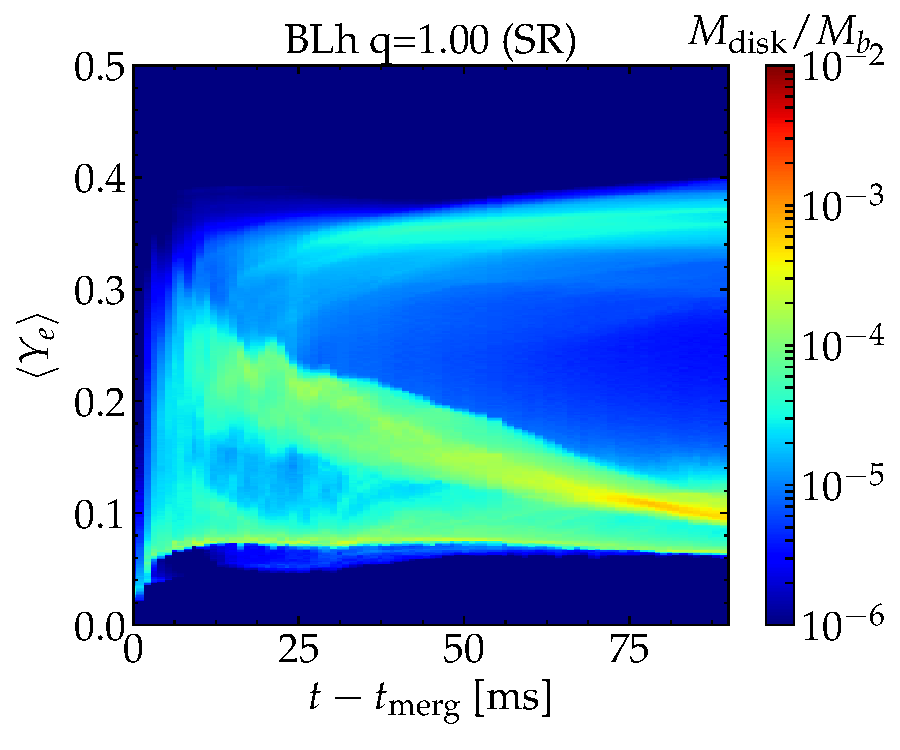
\includegraphics[width=0.49\textwidth]{disk/final_disk_timecorr_blh_q1_Lk.pdf}
    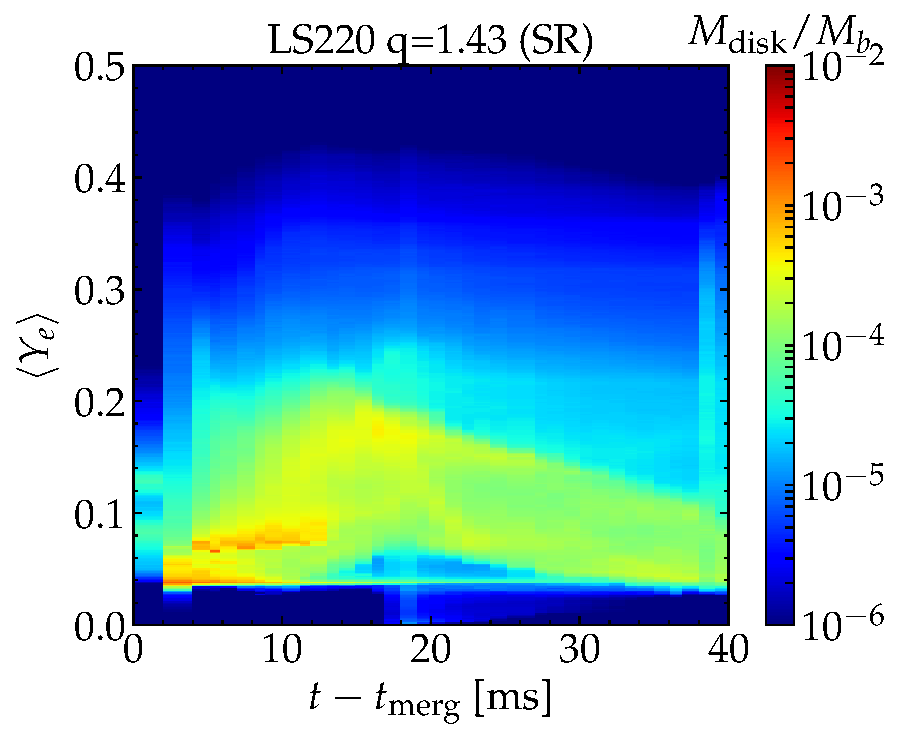
\includegraphics[width=0.49\textwidth]{disk/final_disk_timecorr_ls220_q14_LK.pdf}
    \caption{
        Evolution of the mass-averaged electron fraction, $Y_e$, in 
        the disk of two models, BLh $q=1.00$ and LS220 $q=1.43$ shown on the 
        \textit{left panel} and \textit{right panel}, that produce 
        long- and short-lived remnants respectively.
        %
        The plot shows that during the \pmerg{} evolution, neutrino 
        cooling lowers the $Y_e$ of the bulk of the disk matter. 
        A small fraction of the disk, however, reaches higher $Y_e$, 
        while being irradiated by neutrinos and processed by shocks 
        %
        (Adapted from \citet{Nedora:2020pak}).
        %        Evolution of the disk mass-averaged electron fraction with
        %        time for a long-lived (top) and a short-lived (bottom)
        %        remnant. The plot shows that with time the bulk of the disk lowers
        %        its $Y_e$ via cooling, while a small fraction in terms of mass
        %        gains a high $Y_e$, which relates to the highly 
        %        irradiated surface of the disk. Adopted from \citet{Nedora:2020pak}.
    }
    \label{fig:total_disk_time_corr_Ye_Blh_q1}
\end{figure}

\begin{figure}[t]
    \centering 
    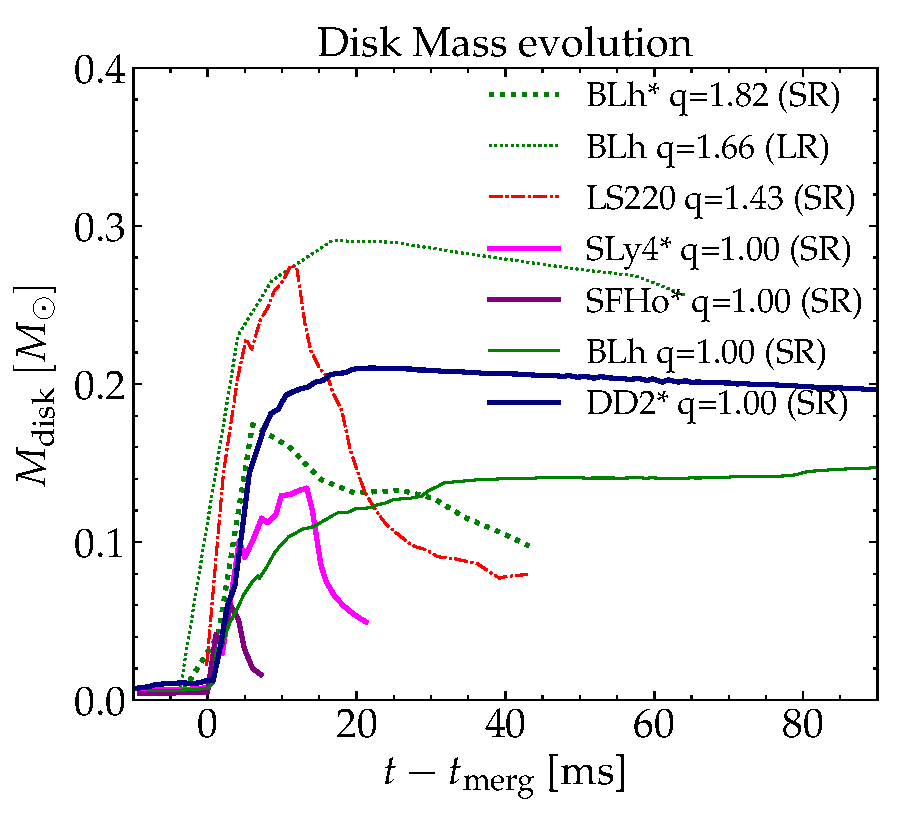
\includegraphics[width=0.49\textwidth]{disk/total_disk_mass_evo.pdf}
    \caption{
        Time evolution of the mass of the disk for a representative list 
        of simulations, that includes those that produce long-lived 
        remnants, \eg, DD2* $q=1.00$, short-lived remnants, 
        \eg, SLy4* $q=1.00$, and a simulation that undergoes \ac{PC}, 
        BLh* $q=1.82$. 
        %
        The plot shows that the \pmerg{} evolution of disk mass depends 
        strongly on the remnant. If the remnant is a \ac{NS}, the disk is 
        accreted slowly and its mass remains almost unchanged by the end 
        of our simulations, while if \ac{BH} forms, the disk is accreted 
        rapidly (if \mr{} is not large).
%        Time evolution of the total disk mass for a few selected
%        short-lived and long-lived cases. The former show a rapid 
%        accretion right after disk formation. The plots show
%        distinct difference in dynamical evolution after disk formation: accretion onto
%        the newly formed BH (short-lived remnants) or accretion onto the NS
%        remnant (DD2 $q=1$) with possible continuous mass shedding from the remnant
%        into the disk (BLh* $q=1$). 
        (Adapted from \citet{Nedora:2020pak}).
    } 
    \label{fig:disk_mass_evo}
\end{figure}

In Fig.~\ref{fig:disk_ang_mom_flux_map_blh_q1} we show how the angular momentum is 
being transported from the \ac{NS} remnant into the disk 
%with its flux defined as $J_r = T_{ra}(\p_\phi)^a$
in two models with long-lived 
\ac{NS} remnants: %and included turbulent viscosity:
DD2* $q=1.00$ and BLh* $q=1.00$.
%
%These are the models with DD2 \ac{EOS} $q=1.00$ and BLh \ac{EOS} $q=1.00$.
%
The angular momentum is transported via spiral waves, 
shown in Fig.~\ref{fig:ang_mom_flux}, induced by the 
$m=1$ and $m=2$ hydrodynamic modes, discussed above.
%
We observer that in the model with more stiff \ac{EOS}, %DD2
the fist wave is considerably stronger. 
%Notably, the DD2 $q=1.00$ model also has a more massive disk.

%%%% MOVED DOWN
%The evolution of the disk-remnant interactions after ${\sim}20\,$ms \pmerg{} 
%is different for two models. While in the DD2* $q=1.00$ model the 
%accretion takes starts to dominate over mass shedding,
%in the BLh $q=1.00$ model the mass shedding prevails till 
%the end of the simulation.
%%shedding mass into its disk stops and accretion begins, in the model with BLh \ac{EOS} the mass shedding does not terminate 
%%continues to shed mass into the disk (see Fig.~\ref{fig:disk_mass_evo}).
%% and discussion in Sec.~\ref{sec:bns_dynsmics_overview})
%%
%The latter is caused by the strong angular momentum flux 
%%\red{actually the plot shows, that it is not}, 
%emanating from the \ac{NS} remnant.
%This might be attributed to the larger temperatures 
%that a model with BLh \ac{EOS} can reach (See Sec.~\ref{sec:nr_methods:eos}). 
%%
%Larger temperatures lead to lower rotational frequency at which the mass 
%shedding occurs \citep{Kaplan:2013wra}. 

The subgrid turbulence enhances the angular momentum transport. 
However more simulations of long-lived 
\ac{NS} remnants are needed to asses the effects of the 
subgrid turbulence and \mr{} systematically. 


%\subsubsection{High \mr{} binaries}

%\subsection{The evolution of remnant-disk interactions}
%\subsection{Remnant-disk evolution}

%\subsubsection*{High mass ratio binaries}
%\subsection{High mass ratio binaries}

%% --- On THE PROMPT collapse
We find that in models with high \mr{}, $q\gtrsim1.67$, the companion star (less 
massive one) undergoes tidal disruption before merger as tidal forces overcome the star's 
binding energy, creating a disk around the primary.
The disk accretion pushes the remaining \ac{NS} mass beyond the 
maximum supported limit by the \ac{EOS}, which leads to a \ac{PC}. 
%These are so-called, prompt collapse cases \citep{Radice:2020ddv,Bernuzzi:2020tgt,Bernuzzi:2020txg}.
These models are characterized by a monotonic increase in their 
central density during the merger.
%The newly formed \ac{BH} is surrounded by the accretion disk that was 
%left from the tidally disrupted companion.
%
At formation, the disk is massive, ${\sim}0.15\,\Msun$, in comparison with 
disks fromed in \ac{PC} of equal mass binaries \citep[\eg][]{Radice:2018pdn}, 
and is also very neutron-rich, $Y_e\sim 0.1$.  
%
%and we discuss it separately for low \mr{} and high \mr{} binaries.
%The evolution of the disk mass is shown in Fig.~\ref{fig:disk_mass_evo}.

%\subsubsection*{Binaries with $q\lesssim1.4$}
%\subsection{Binaries with $q\lesssim1.4$}

Binaries with small mass ratio, $q\lesssim1.4$,
produce either a short- or a long-lived remnant depending  
on the \pmerg{} configuration and properties. 
%produce a \ac{NS} remnant
%%that either survives on a dynamical timescale, set by the \ac{NS} rotation, before
%collapsing to a \ac{BH}, or a \ac{NS} remnant that survives till the end of the simulations.
%We refer to the former ones as \textit{short-lived} and the latter ones as %% ---------- Defind Above
%\textit{long-lived} remnants.
%
Most binaries producing short-lived remnants have relatively soft \acp{EOS}
and small \mr{}s, \eg, models LS220 $q=1.1, \,q=1.2$, SFHo $q=1.1, \,q=1.4$, 
and SLy $q=1.1,\, q=1.4$. They collapse within ${\sim}20$~ms \pmerg. 
The exact time of the collapse however depends on the simulation resolution 
and on the inclusion of subgrid turbulence as was previosly noted by \citet{Radice:2017zta}.






%\subsubsection*{Disk of short-lived remnants}
%\subsection{Disk of short-lived remnants}

%During the merger, shocks, generated at the collisional interface of the \ac{NS} cores,
%as well as, tidal torques exerted by the non axisymmetric remnant, result in a formation
%of the disk. Matter, energy and angular momentum are injected into the disk as the spiral 
%density waves propagate outwards from the mass-shedding \ac{NS} remnant 
%\citep{Bernuzzi:2015opx,Radice:2018xqa}.
%
%\red{HERE the letter stuff could be added, actually}
%
% --- Letter stuff
%The spiral arms extend from the \ac{NS} remnant into the disk and transport angular 
%momentum outwards as shown in Fig.~\ref{fig:ang_mom_flux}. %Such global density waves are --- written above 
%a generic and efficient mechanism to redistribute energy and eventually deplete  
%accretion disks \citep{Goodman:2001a,Rafikov:2016a,Arzamasskiy:2018a}. 
%% Crucially, we find that both the $m=1$ and $m=2$ modes generate a \wind{} from the
%% disk's outer layers that is distinct from the dynamical ejecta, see Fig.~\ref{fig:ej_properties}.
%
% <<< MOVED TO INTRO >>>
%
%The maximum values of fluid temperature in the disk are reached within 
%the spiral waves. During the \pmerg{} evolution, the disk expands and 
%cools via neutrino emission.
%High temperatures lead to the electron-positron pair creation, 
%%% [added from Shibata Review paper]
%facilitating the positron capture by free neutrons 
%%$n+e^+ \rightarrow p +\bar{\nu}_e$ 
%in the disk.
%%
%The average particle energies are large, close to the mass difference between neutron 
%and proton. 
%The entropy per baryon varies between $3$ and $\lesssim 10\,$$k_{B}$/baryon \citep{Perego:2019adq}.
%In combination with the high $\nu_e$ and $\bar{\nu}_e$ luminosities,
%the large number of available positrons leads to an increase 
%in the fluid electron fraction, $Y_e$, in relation to the initially neutron-rich material
%\citep{Qian:1996xt}.
%This process is called deleptonization. 
%%
%Additionally, a \ac{NS} remnant itself is a strong neutrino emitter. The neutrino irradiation of the 
%surrounding area alters its composition, as neutrons and protons absorb the neutrinos,
%$n+\nu_e\rightarrow p + e^{-}$ and $p + \bar{\nu}_e\rightarrow n + e^+$.
%This drives the neutron and proton fraction towards equilibrium, and raises the $Y_e$.
%%\red{paper says: 
%%    The electron fraction is reset by an initial excess of electron antineutrino emission
%%    and electron neutrino absorption,}
%% ---
As we discussed in Sec.~\ref{sec:intro:merg_pmerg}, the strong neutron fluxes 
emanating from the remnant and the hot disk matter raises the fluid electron fraction. 
%
If a \ac{NS} remnant collapses to a \ac{BH}, the main source of neutrinos shuts down,  
the inner part of the disk accrets rapidly, and the disk itself moves to a 
quasi-steady state with axisymmetric, approximately Keplerian profile. 
%(see Fig.~\ref{fig:disk_mass_evo}).
%
Indeed, in our models we find, that the inner part of the \pmerg{} disk, 
at densities $\rho\sim10^{13}\,$\gcm{}, is relatively hot, $T\sim10\,$MeV, 
but neutron-rich $Y_e\sim0.1$, as it remained shielded from the neutrino irradiation. 
The matter gets progressively colder and proton-rich outwards, 
with $Y_e$ reaching $0.4$ at the edges.
%
Our analysis of two representative models, 
BLh $q=1.00$ and LS220 $q=1.43$, corraborates this picture. 
%
The evolution of the mass-weighted electron fraction 
for these models is shown in Fig.~\ref{fig:total_disk_time_corr_Ye_Blh_q1}, 
%
where former model has been evolved till ${\sim}90$~ms \pmerg{}. 
%
During the formation, shocks and spiral waves raise the disk electron fraction to
$Y_e\sim0.25$. As the disk evolves, the bulk of its mass, shielded from neutrinos, 
%(Fig.~\ref{fig:slice:heating_hu}, density contours) 
returns to neutron-rich condition with $Y_e\lesssim0.1$. The outer part of the disk, 
however, is subjected to the strong neutrino irradiation and reaches $Y_e\sim0.4$ on a 
timescale of ${\sim}40$~ms\footnote{
    The apparent gap in the $Y_e$ distribution in 
    Fig.~\ref{fig:total_disk_time_corr_Ye_Blh_q1} at $\langle Y_e \rangle \simeq 0.15$ 
    might not be of physical origin, but an artifact from the neutrino M0 scheme, 
    that assumes neutrinos propagate along the radial directions
    (see Sec.~\ref{sec:nr_methods:neut}), that is not well suited for capturing the 
    neutrino emission and re-absorption from the disk midplane.
}.
%% Note that neutrinos in merger remnants decouple at $\rho\sim10^{11}$~$\gccm$ \citep{Endrizzi:2019trv}. 
%
In case of the LS220 $q=1.43$ models that produces a short-lived \ac{NS} remnant 
the average electron fraction is lower as the main source of neutrinos collapses 
shortly after merger.



The disk mass at formation shows dependency on the \ac{NS} \ac{EOS}. Specifically, 
binaries with stiffer \acp{EOS} (larger \ac{NS} radii) produce more massive disks. 
Additionally, the disk mass depends on \mr{}. For instance, the most massive 
disks are formed in LS220 $q=1.43$ and BLh $q=1.82$ models.
%
The disk accretion onto a \ac{BH} removes up to 
$50\%$ of its mass on a timescale of tens of milliseconds.


%% -- 
%\subsubsection*{Disk of long-lived remnants}
%\subsection{Disk of long-lived remnants}

If the \ac{NS} remnant is long-lived, the disk has time to complete its formation,
and thus it is more massive and extended \citep{Perego:2019adq}. 
%As before, the disk is defined as matter, with $\rho\lesssim10^{13}$~\gcm. 
The final mass is higher for models with larger \mr{}s and stiffer \acp{EOS}.
For instance, 
in the BLh $q=1.00$ model
%for the model with $q=1.00$ and BLh \ac{EOS}, 
the disk mass reaches ${\lesssim}0.15\,\Msun$, while in the 
%model with $q=1.00$ and DD2 \ac{EOS} 
DD2 $q=1.00$ model 
it exceeds ${\sim}0.2\,\Msun$. For models with BLh \acp{EOS}, 
the disk mass increases between $q=1.00$ and $q\sim1.4-1.5$ by a $100\%$.

%The evolution of the disk-remnant interactions after ${\sim}20\,$ms \pmerg{} 
%is different for two models. While in the DD2* $q=1.00$ model the 
%accretion takes starts to dominate over mass shedding,
%in the BLh $q=1.00$ model the mass shedding prevails till 
%the end of the simulation.
%%shedding mass into its disk stops and accretion begins, in the model with BLh \ac{EOS} the mass shedding does not terminate 
%%continues to shed mass into the disk (see Fig.~\ref{fig:disk_mass_evo}).
%% and discussion in Sec.~\ref{sec:bns_dynsmics_overview})
%%
%The latter is caused by the strong angular momentum flux 
%%\red{actually the plot shows, that it is not}, 
%emanating from the \ac{NS} remnant.
%This might be attributed to the larger temperatures 
%that a model with BLh \ac{EOS} can reach (See Sec.~\ref{sec:nr_methods:eos}). 
%%
%Larger temperatures lead to lower rotational frequency at which the mass 
%shedding occurs \citep{Kaplan:2013wra}. 

The long-term evolution of the disk is driven by its interaction with the \ac{NS} remnant 
remnant and cooling. If the central remnant is a \ac{BH}, the only possible 
interaction is the disk accretion onto a \ac{BH}, while in the case of a \ac{NS} remnant 
the picture is more complex.
%
Neutrino cooling and gravitational pull from the remnant facilitates the 
accretion. Simultaneously, spiral density waves inject %generated at shocks,
energy and angular momentum into the disk as well as centrifugally supported 
material, heating up and expanding it.  %(the \ac{NS} remnant undergoes mass-shedding). 
This is the case for DD2* $q=1.00$ and BLh $q=1.00$ models where the quasi-steady 
state disk accretion and mass-shedding maintain the disk mass almost constant 
till the end of the simulation, as depicted in Fig.~\ref{fig:disk_mass_evo}.
%
%In Fig.~\ref{fig:disk_mass_evo} the quasi-steady state disk accretion
%is seen for the DD2 $q=1.00$ model. Meanwhile, the mass-shedding 
%by the remnant adds more material into the disk than is being accretted as is the 
%case for the model with BLh \ac{EOS} and $q=1.00$. 
%
The strong mass-shedding in BLh $q=1.00$ model can be attributed to the very 
high average temperatures of the remnant and the disk reached in this model, 
that are a consequence of the thermal 
effects included in the BLh \ac{EOS} (see Sec.~\ref{sec:nr_methods:eos}), and the 
softness of the \ac{EOS}, which leads to the strong oscillations of the remnant 
after merger, as discussed above. Larger temperatures lead to lower rotational 
frequency at which the mass shedding occurs \citep{Kaplan:2013wra}. 
%(see Sec.~\ref{sec:bns_sims:dens_modes}).

The inclusion of the subgrid turbulence smears the mass distribution of disk 
properties. The distributions of electron fraction, entropy per baryon and 
temperature appears broader. A more detailed quantitative analysis would require more 
simulations performed at several resolutions to disentangle the effects 
caused by the subgrid turbulence and by the finite grid \citep{Bernuzzi:2020txg,Radice:2020ids}.


%%%%% <<< MOVED ABOVE
%\subsection{Evolution of disk properties and disk final structure}
%%\subsection{Evolution of disk properties}
%
%%% Ye evolution
%The evolution of the mass-weighted electron fraction in the 
%%the model with BLh \ac{EOS} and $q=1.00$, 
%BLh $q=1.00$ and LS220 $q=1.43$ models is shown in 
%Fig.~\ref{fig:total_disk_time_corr_Ye_Blh_q1}, 
%%
%where former model has been evolved till ${\sim}90$~ms \pmerg{}. 
%%
%During the formation, shocks and spiral waves raise the disk electron fraction to
%$Y_e\sim0.25$. As the disk evolves, the bulk of its mass, shielded from neutrinos, 
%%(Fig.~\ref{fig:slice:heating_hu}, density contours) 
%returns to neutron-rich condition with $Y_e\lesssim0.1$. The outer part of the disk, 
%however, is subjected to the strong neutrino irradiation and reaches $Y_e\sim0.4$ on a 
%timescale of ${\sim}40$~ms\footnote{
%    The apparent gap in the $Y_e$ distribution in 
%    Fig.~\ref{fig:total_disk_time_corr_Ye_Blh_q1} at $\langle Y_e \rangle \simeq 0.15$ 
%    might not be of physical origin, but an artifact from the neutrino M0 scheme, 
%    that assumes neutrinos propagate along the radial directions
%    (see Sec.~\ref{sec:nr_methods:neut}), that is not well suited for capturing the 
%    neutrino emission and re-absorption from the disk midplane.
%}.
%%% Note that neutrinos in merger remnants decouple at $\rho\sim10^{11}$~$\gccm$ \citep{Endrizzi:2019trv}. 
%%
%In case of a 
%LS220 $q=1.43$ models that produces a 
%short-lived \ac{NS} remnant  % model with LS220 \ac{EOS} and $q=1.43$ 
%(right panel of the Fig.~\ref{fig:total_disk_time_corr_Ye_Blh_q1})
%the average electron fraction is lower as strongly irradiating remnant the 
%collapses shortly after merger. 
%%
%%Additionally, the outskirts of the more compact disk remain 
%%at low electron fraction as the neutrino emitted by the disk itself 
%%%%are the only source of neutrinos. 

%\end{document}

%% -----------------------------------------------
%%
%% F I N A L  D I S K  S T R U C T U R E
%%
%% -----------------------------------------------

\subsection{Final disk structure}
%\subsection{Final disk structure}

\begin{figure}[t]
    \centering
    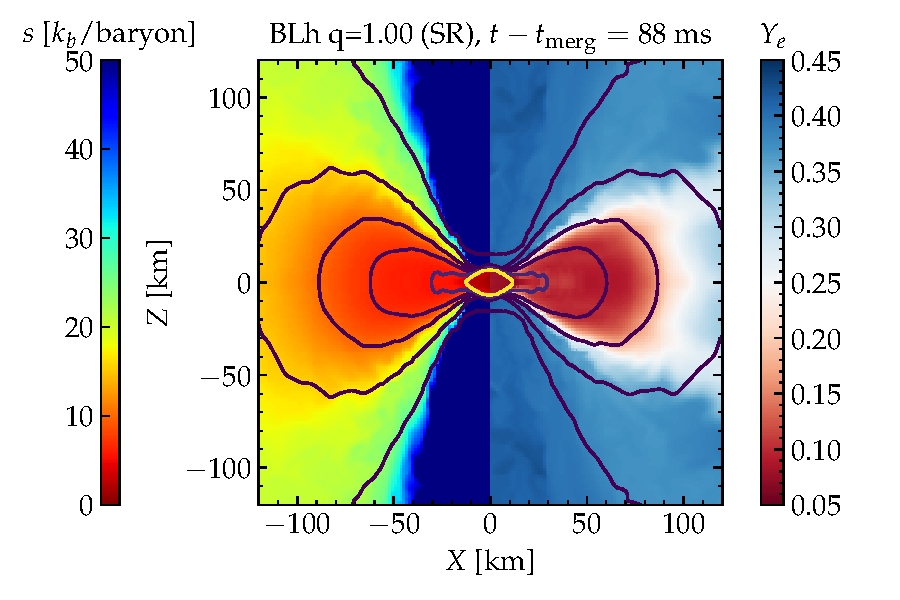
\includegraphics[width=0.49\textwidth]{disk/final_structure/slice_xz_entr_ye_blh_q1_rl3.pdf}
    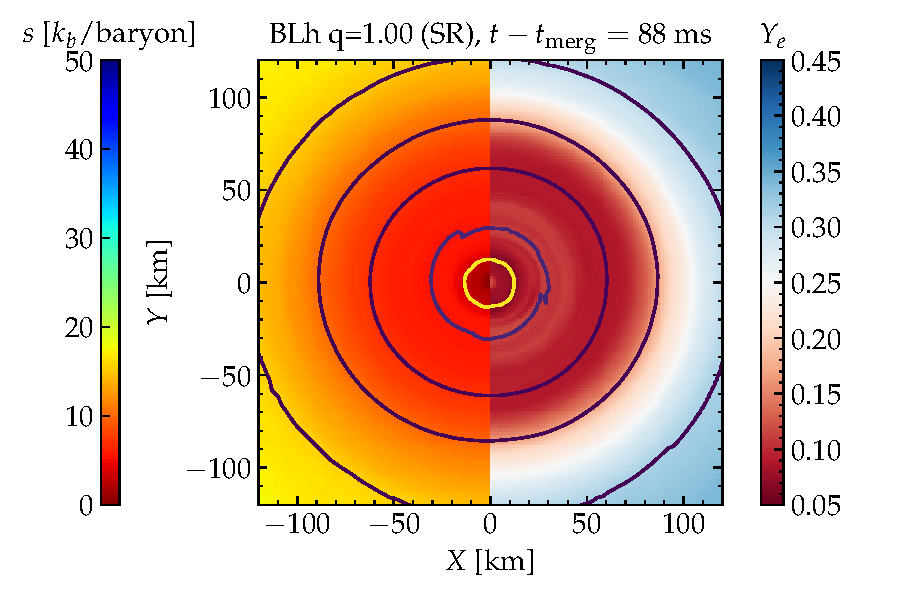
\includegraphics[width=0.49\textwidth]{disk/final_structure/slice_xy_entr_ye_blh_q1_rl3.pdf}
    \caption{
        Snapshots of disk properties on $(x,z)$ \textit{left panel} and 
        $(x,y)$ \textit{right panel} for BLh $q=1.00$ model, taken 
        $88\,$ms \pmerg{}. 
        %
        On each panel, the entropy per baryon is shown on the left 
        side of the panel, and the electron fraction -- on the right. 
        %
        Solid contours mark the rest mass density values, that from the 
        innermost yellow contour, encompassing the remnant, read 
        $[10^{13}, 10^{12}, 10^{11}, 10^{10}, 10^{9}]$ g cm$^{-3}$.
        (Adapted from \citet{Nedora:2020pak}). 
%        Entropy and electron fraction on the $(x,z)$ (top) and
%        $(x,y)$ planes (bottom) for the remnant of BL $q=1$ at the end
%        of the simulation. Each plot is divided vertically, with entropy
%        being color-coded on the left and electron fraction on the
%        right. Solid contours stand for rest muss density. Counting from
%        the center, the values are $[10^{13}, 10^{12}, 10^{11}, 10^{10},
%        10^{9}]$ g cm$^{-3}$, with the inner most contour encompassing
%        the remnant.
%        (Adapted from \citet{Nedora:2020pak})
    }  
    \label{fig:snapshots_xy_ye_entr}
\end{figure}

\begin{figure*}[t]
    \centering 
    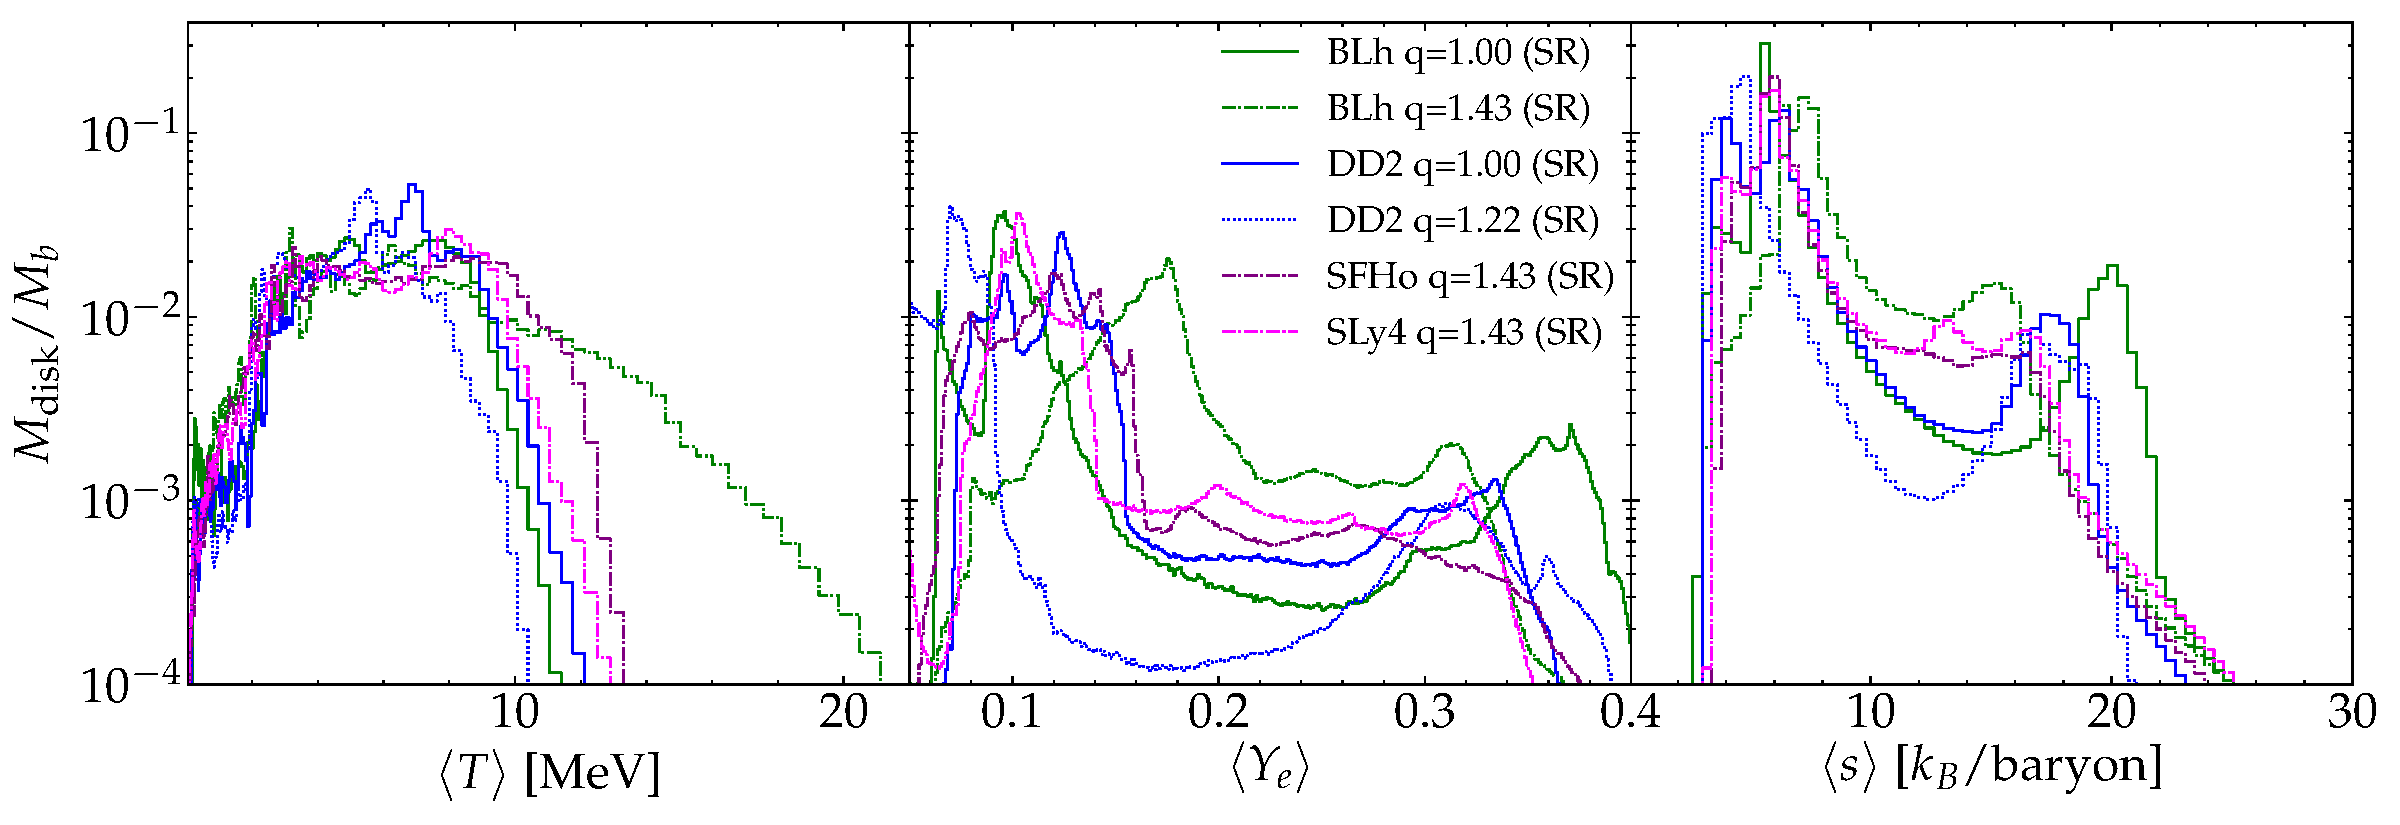
\includegraphics[width=0.95\textwidth]{disk/final_structure/disk_hist_shared.pdf}
    \caption{
        Disk properties in the form of mass histograms 
        at the end of evolution for a set of simulations.
        From left to right, panels depict the temperature, $T$, 
        fraction $Y_e$ and entropy $s$. 
        (Adapted from \citet{Nedora:2020pak}).
%        \textit{Left panel} shows the temperature, $T$, 
%        \textit{middle panel} depicts the, 
%        
%        Composition of the disks at the end of the long-lived
%        remnants simulations. The histograms refer to the temperature $T$
%        (left),
%        electron fraction $Y_e$
%        (middle) and entropy $s$ (right).
%        (Adapted from \citet{Nedora:2020pak})
    }
    \label{fig:final_disk_struct_hist_long}
\end{figure*}

%In this section we discuss the final structure and properties of the disk, 
%focusing on the models with long-lived \ac{NS} remnants.
%The properties are extracted at typical time $\sim60{-}100$~ms after merger.
%
From the density contours in Fig.~\ref{fig:snapshots_xy_ye_entr}, 
we observe that even at ${\sim}88\,$ms after merger the disk
of the BLh $q=1.00$ model remains geometrically thick. 
%We find that the generally the disk is optically thick.
Comparing with other models we note that 
the disk' \ac{RMS} half-openning angle appears to be independent of the 
\ac{EOS} and \mr{} and is $\langle\theta\rangle_{\text{rms}}\sim60^{\circ}$. 
The radial extend of the disk, however increases with the \ac{EOS} softness and $q$.
%
Similarly, the final disk mass is larger for the unequal mass binaries, 
ranging overall between ${\sim}0.1\,M_{\odot}$ and ${\sim}0.4\,M_{\odot}$
(see Tab.~\ref{tab:sim}) and is larger in the case of long-lived remnants.

%
We examine disk mass dependencies on binary parameters in Appendix~\ref{ch:stat}, 
Sec.~\ref{sec:stat:remdisk}, where we combine our data with the data available in 
the literature and show that the aforementioned dependencies on $q$ and $\tilde{\Lambda}$ 
can be captured by a simple two parameter, second order polynomial in this quantities. 
%
The systematics in data, however, are large, and while in comparison with other fitting 
formulae available in the literate, the polynomial performs better, 
significantly larger sample of simulations with advanced physics and consistent method 
of disk mass extraction is required for constraining the polynomial, especially at the 
known boundaries of the parameter space, \eg, $\tilde{\Lambda}\rightarrow0$.

%than short-lived ones as \ac{BH} accretion removes ${\sim}50\%$ 
%of the mass in the latter case.
%
%Notably, for models with long-lived remnants the disk mass is larger,
%that for the those with short-lived remnants. This can be attributed to the 
%rapid accretion onto a \ac{BH} that removes $\sim50\%$ of the disk mass.
%
%We investigate the overall statistical properties of the disk mass for all our models
%and compare them to those available in the literature in Sec.~\ref{sec:stat:remdisk}
%
%\gray{
%    The mean value of the disk mass in out models is 
%    $\overline{M}_{\text{disk}}=(0.161 \pm 0.083)M_{\odot}$,
%    where the standard deviation is also reported.
%    %% ---
%    Similarly to the dynamical ejecta we fit the disk masses with the 
%    second order polynomial in $(q,\tilde{\Lambda})$.
%    The coefficients of Eq.~\eqref{eq:fit:poly22}
%    for this fit are given in Tab.~\ref{tab:fitpoly22coefs}.
%    A more detailed study with various fitting formulas and extended
%    datasets from the literature is reported in a companion paper.
%}

%Next, we consider the composition of the disk at the end of the simulation.
%
The mass-averaged temperature, electron fraction and entropy per baryon
for several representative models are presented in Fig.~\ref{fig:final_disk_struct_hist_long}.
%
The plot shows that the mass-weighted distribution of the entropy and electron 
fraction have a bimodal structure, more pronounced in the case of 
equal mass binaries. 
The low entropy, $s\sim5-10\,k_B/$baryon, peak corresponds to the bulk, mildly shocked, 
material, while the higher entropy peak, $s\sim15-22\,k_B/$baryon, marks 
the strongly shocked material. Notably, the former is largely independent of 
\ac{EOS} and \mr{} while the latter is more pronounced in models with softer \ac{EOS}. 

%
%Notably, in models with higher \mr{}, 
%the second peak is located at lower $s$. 
%
%The mass-weighted distribution 
%of the electron fraction displays a similar double-peak structure.
Similarly, the low $Y_e$ peak, $Y_e\sim0.1$, corresponds to the neutrino-shielded part of the 
disk, while the high $Y_e$ peak, $Y_e\sim0.3-0.4$, marks the outer parts of the disk,
where fluid is subjected to the strong neutrino irradiation.
%
Comparing the disk properties with the 2D snapshots of the electron fraction 
and density within the disk shown in Fig.~\ref{fig:snapshots_xy_ye_entr}, we observe, 
that indeed, the two peaks in the mass-weighted distribution of these quantities 
correspond to different regions within the disk.
%
%In Fig.~\ref{fig:snapshots_xy_ye_entr} we show the electron fraction 
%and entropy per baryon on the $xy$ and $xz$ slices of the equal 
%mass model with BLh \ac{EOS}. The plot shows, that the two peaks in the 
%mass-weighted distribution of electron fraction and entropy correspond to 
%different regions within the disk.

With respect to the temperature, we find that 
most of the disk matter has temperature of $T\sim 1-10\,$MeV with the 
innermost parts being hotter then the outermost ones. 
The disk temperature distribution appears to be largely 
independent of the \ac{EOS} and \mr{}.



%% -----------------------------------------------
%%
%% E X P E C T E D  M A S S  E J E C T I O N
%%
%% -----------------------------------------------

%\subsection{Mass ejection on a longed timescale}
\subsection{Mass and angular momentum loss}\label{sec:bns_sims:mj_loss}

%As the disk expands and cools, the recombination of nucleons into alpha particles 
%starts to take place. The energy, released in recombination, might be sufficient 
%for the outermost layers to become unbound, generating an outflow and contributing 
%to the disk depletion \citep{Beloborodov:2008nx,Lee:2009uc,Fernandez:2013tya}.
%%
%This process, however, is expected to take place on timescales longer than
%those simulated here. 
%Additionally, an outflow induced by viscous heating within the disk and 
%so-called neutrino-driven wind (\nwind{}; \citet{Dessart:2008zd,Perego:2014fma,Just:2014fka})
%driven by neutrino heating above the remnant, are expected to contribute to the 
%mass and angular momentum mass loss. 

%and by the dynamical
%interactions between the \ac{NS} remnant and the disk, the \swind{} \citep{Nedora:2019jhl}.
%
%We discuss the properties of the ejecta in the next section, 
%Sec.~\ref{sec:bns_sims:ejecta}.

%We discuss the properties of the \nwind{} found in our simulations
%in Sec.~\ref{sec:bns_sims:nwind} and the properties of the 
%\swind{} in Sec.~\ref{sec:bns_sims:sww}.
%
%The \swind{} can have a mass up to
%a few $10^{-2}\,\Mo$ and velocities ${\sim}0.2$~c. The ejecta
%have electron fraction typically larger than ${\sim} 0.25$ since they are 
%partially reprocessed by hydrodynamic shocks in the expanding arms. 
%The \nwind{} is driven by neutrino heating above the remnant. It generates outflows
%with smaller masses ${\sim} 10^{-4}M_{\odot}$ and larger $Y_e$
%than the \swind{}. 
%Differently from \swind{} the mass flux of the \nwind{} in our simulations subsides 
%before the end of out simulations, due to rapid baryon loading of the 
%polar region.
%The \swind{} will be discussed in detail in Sec.~\ref{sec:spiralw}.
%The effects of these outflows on the dynamical evolution of the remnant 
%lies in the amount of mass and angular momentum they can remove from the system.
%
%Specifically, the \nwind{} have a typical mass of ${\sim} 10^{-4}\,\Msun$, 
%while the \swind{} could remove $10^{-2}\,\Msun$ on a timescale of a ${\sim}100\,$ms.

\begin{figure}[t]
    \centering 
    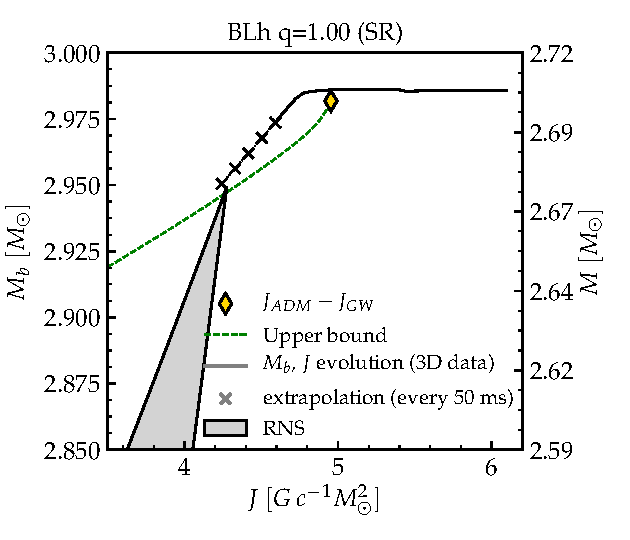
\includegraphics[width=0.59\textwidth]{ejecta_sec/secular_j_mb_RNS_blh.pdf}
    \caption{
        Evolution of the BLh $q=1.00$ \pmerg{} remnant $J$-$M_b$ space, where 
        $J$ is the total angular momentum, $M_b$ is the baryonic mass, 
        depicted with the solid black line. The evolution begins in the 
        upper right corner and proceeds towards the lower left one, as the 
        remnant looses, first angular momentum to \ac{GW} emission, than, 
        both $J$ and $M_b$ to massive winds. The point where the \ac{GW}-phase 
        ends is marked with yellow marker. 
        The end of the black solid line indicates the end of our simulation. 
        We linearly extrapolate the evolution trajectory, and plot it with black crosses. 
%        Baryon mass vs angular momentum diagram for the BLh $q=1$ remnant.
%        The colored diamond marks the baryonic mass and angular momentum at the end
%        of the dynamical gravitational-wave dominated phase.
%        After the GW phase, the evolution is driven by the massive outflows.
%        The solid black line is the $M_b$ and $J$ estimated from the 3D data
%        integrals under the assumption of axisymmetry.
        The green dashed line is a conservative estimate
        of the mass ejection and a possible trajectory for the viscous
        evolution as estimated in \citet{Radice:2018xqa}. 
%        The crosses are
%        a linear extrapolation in time of the solid black line. 
        The gray
        shaded region is the region of stability of rigidly rotating \ac{NS} 
        equilibria. 
        (Adapted from \citet{Nedora:2020pak}).
    }
    \label{fig:total_j_mb_rns_blh}
\end{figure}
%        \footnote{
%            \url{http://www.gravity.phys.uwm.edu/rns/#:~:text=RNS%20is%20a%20code%20written,are%20supplied%20by%20the%20user.}
%        }
Quantitative understanding of the long-term \pmerg{} dynamics 
requires ab-initio \ac{NR} simulations in $(3+1)$D with compete physics.
%
Here we asses a possible long-term evolution via an indirect method, 
focusing on the BLh $q=1.00$ (\texttt{SR}) model, one of the longest runs 
performed. 

In this simulation, after the merger, a \ac{NS} remnant is born with an excess 
in baryon mass with respect to the beta-equilibrium \ac{NS} configurations.
%
In Fig.~\ref{fig:total_j_mb_rns_blh} we show the evolution of the 
total baryon mass, $M_b$, and total angular momentum, $J$, of this remnant
(black solid line). 
%
The total $J$ and $M_b$ are evaluated in cylindrical coordinates assuming 
axisymmetry, accounting for both matter in the remnant and the disk. 
%(see Eq.~\eqref{eq:method:ang_mom} and Eq.~\eqref{eq:method:mdisk},
%in Sec.~\ref{sec:bns_sims:method:ang_mom} and Sec.~\ref{sec:bns_sims:method:disk} respectively for more details).
%
%(for the definition of the latter see Sec.~\ref{sec:bns_sims:method:ang_mom}).
%
At early \pmerg{}, when no substantial mass-loss happened yet, the 
evolution is governed by the emission of \acp{GW}. The remnant loses 
angular momentum retaining constant baryonic mass.
%
In order to evaluate the total amount of angular momentum lost to 
\acp{GW} we perform the frequency-domain integration of the \ac{GW} 
strain with the extraction sphere of $R=400\,\Msun$ using the 
\texttt{strain.py} module of the public library 
\texttt{scidata}\footnote{\url{https://bitbucket.org/dradice/scidata}}.
The method is discussed in 
\citet{Damour:2011fu,Bernuzzi:2012ci,Bernuzzi:2015rla}.
%
%\citet{Damour:2011fu,Bernuzzi:2012ci,Bernuzzi:2015rla}\footnote{
%    The radiated angular momentum is computed from the 
%    multipole moments $N_{lm}$ for the \ac{NR} complex "news function" at infinity. 
%    The $J_{z;\text{rad}}(t)$ is computed as \citep{Damour:2011fu} 
%    \begin{equation*}
%    \Delta J_{z\text{rad}}(t) \frac{1}{16}\sum_{l,m}^{l_{max}}\int_{t_0}^{t} dt' m \mathcal{L}[h_{lm}(t')(N_{lm}(t'))^*],
%    \end{equation*}
%    where $h_{lm}$ is the multipolar metric waveform, 
%    $N_{lm}(t) = dh_{lm}(t) / dt$, the news function, and $l_{max}=8$.
%    The $J$ loss is metric dependent ($h$).
%    The $h$ (strain???) is computed from $\Psi_4(t) = dN/dt = d^2h/dt^2$ by a 
%    frequency-domain integration procedure with a low-frequency cut 
%    $\omega_0 = 0.032/(m_1+m_2)$.
%    The routines used for the calculation are taken from the scientific library
%    \texttt{scidata}, available at \url{https://bitbucket.org/dradice/scidata}.
%}.

Subtracting the angular momentum lost to \acp{GW} from the initial data, 
%\ac{ADM} angular momentum,  %\red{(see \url{https://arxiv.org/pdf/1001.5429.pdf})} 
we obtain the value that is left to the system after the \ac{GW} phase 
(the yellow marker in Fig.~\ref{fig:total_j_mb_rns_blh}\footnote{
    Due to different assumptions in its calculation the agreement 
    with $J$ from the volume integrals is not expected.
}).
%
We observe that at this stage the remnant still has an excess in angular momentum
in comparison with the rigidly rotating \ac{NS} configurations with the same baryon mass 
(gray triangular region in Fig.~\ref{fig:total_j_mb_rns_blh}).
%
The equilibria configurations were computed using the \texttt{RNS} code \footnote{
    \texttt{RNS} is a code written by Nikolaos Stergioulas which constructs 
    models of rapidly rotating, relativistic, compact stars using tabulated 
    \ac{EOS} \url{http://www.gravity.phys.uwm.edu/rns/}.
}.
%
%Similar situation is found for other 
We observe the same situation in all our models.% \citep{Zappa:2017xba,Radice:2018xqa}.

Notably, also the baryonic mass of the \pmerg{} remnant exceeds the 
the maximum mass that a rigidly rotating equilibria could have. 
As we mentioned in Sec.~\ref{sec:intro:merg_pmerg}, such remnant is generally referred 
to as a \ac{HMNS} \citep{Baumgarte:1999cq} 
% following the 
%nomenclature introduced for zero-temperature \ac{EOS} equilibria \acp{NS} \citep{Baumgarte:1999cq}, 
and is expected to collapse to a \ac{BH} shortly after formation. 
%
However, as Fig.~\ref{fig:total_j_mb_rns_blh} shows, a remnant that efficiently 
looses mass sets on a trajectory towards the rigidly rotating, stable configuration. 
%
The extrapolation of the final trend of the mass and angular momentum loss shows that 
if ${\approx}0.05\,\Msun$ (${\approx}40$\% of the final disk at the end of the simulation) is 
ejected, the \ac{NS} remnant would approach the rigidly rotating equilibria region 
at the mass-shedding limit (gray-shaded region in Fig.~\ref{fig:total_j_mb_rns_blh}). 
%
Extrapolation indicates, that if the ejecta mass flux does 
not change, this would occur on a timescale of ${\sim}350$~ms \pmerg{}.
%
Thus, in principle, a \ac{HMNS} remnant can avoid the collapse. 
This calls for a more detailed investigation with long-term \ac{NR} \ac{BNS} 
merger simulations that employ advanced physics.

%
%However, as Fig.~\ref{fig:total_j_mb_rns_blh} shows, the remnant that efficiently 
%losses mass, can avoid the collapse, if the \ac{RNS} concan avoid the 
%collapse by efficiently removing angular momentum and mass, and can reach the 
%rigidly rotating equilibria phase.% in a ${\sim}350\,$ms.
%avoiding the collapse.
%
%
%We compute the angular momentum and baryon mass evolution of the remnant 
%through volume integrals, assuming axisymmetry and evaluating the former using 
%Eq.~\eqref{eq:method:ang_mom}, and the latter using the Eq.~\eqref{eq:method:mdisk},
%relaxing the rest-mass density criterion. 
%The evolution of these two quantities is depicted with the black solid line if 
%Fig.~\eqref{fig:total_j_mb_rns_blh}~\footnote{
%    Note that the angular momentum estimated
%    from the \ac{GW} and from the integral of Eq.~\eqref{eq:method:ang_mom} assuming
%    axisymmetry are compatible within the errors made in the latter estimate.
%}.

The massive outflow that starts to dominate the \pmerg{} dynamics after the \ac{GW}-phase 
is driven by the interaction between non-axisymmetric 
remnant, subjected to $m=1$ and $m=2$ instabilities, and the disk.
We call this outflow \ac{SWW} and examine its properties in detail in the next section. 

%
%
%Similar results are obtained with the conservative upper bound estimate on the 
%evolution of the long-lived remnant (Eq.~$2$ in \citet{Radice:2018xqa}) (green dashed line in 
%the figure). 

Additionally, we estimate a conservative upper bound evolution of the 
long-lived remnant based on the following considerations \citep{Radice:2018xqa}.
%
%%%% From Radice18 paper on ViscousEjecta
%A more conservative estimate can be obtained assuming
%that the material becomes unbound due to the recombination
%of nucleons into nuclei and the subsequent liberation of
%nuclear binding energy, a scenario discussed in detail in 
%Beloborodov (2008), Lee et al. (2009), and Fernandez \& Metzger
%(2013), among others. This has been shown to occur
%once the material has reached a cylindrical radius $r*$ at
%which the nuclear recombination energy equals the gravitational
%binding energy (Lee et al. 2009; Fernandez & Metzger 2013), that is
%
%\begin{equation}
%    \frac{G M m_b}{r*} \approxeq 8.8\, \text{MeV}
%\end{equation}
%
%In the previous equation $M$ is the central object mass and
%$m_b$ is the average baryon mass. Accordingly, a ring of material
%initially orbiting at radius $r < r*$ and becoming unbound
%would carry away, in addition to its specific angular
%momentum $j(r)$, also the angular momentum needed to expand
%to $r*$. Assuming a Keplerian disk, this implies that
%the angular momentum carried away by the ring initially at
%$r$ is
%
%\begin{equation}
%    j*(r) = j(r) \Big( \frac{r*}{r} \Big)^{1/2}
%\end{equation}
%
%We take $r* = 300 G/c^2M$ as fiducial value, corresponding
%to $M \approxeq 2.5M_{\odot}$. We repeat the tally of angular momentum
%and mass that can be removed from the remnant
%taking into account the previous equation. The results are
%represented by the blue line in Fig. 3 laying inside the allowed
%region for the viscous evolution. This yields an ejecta
%mass of ${\sim}0.05\Msun$for the DD2 (1.35 + 1.35)$\Msun$ binary.
%Our estimate is in good agreement with the results of Fujibayashi
%et al. (2018), who considered the post-merger evolution
%of the same binary with 2D axisymmetric viscous
%GRHD simulations. They estimated the viscous ejecta mass
%to be ${\sim}0.05\Msun$. Note, however, that the mass ejection was
%still ongoing at the end of the simulations presented by Fujibayashi
%et al. (2018), so the total ejecta mass might be
%larger than what they estimated.
The recombination of nucleons into nuclei and the subsequent 
liberation of nuclear binding energy can be a driving force 
of massive outflows. Matter becomes unbound gravitationally 
once it reaches cylindrical radius $r^*$ at which the nuclear recombination energy 
equals the gravitational binding energy
\citep[\eg][]{Fernandez:2013tya}, 
%
\begin{equation*}
    G M m_b / r^* \simeq 8.8\, \text{MeV}, 
\end{equation*}
%
where $M$ the central object mass and $m_b$ is the average baryon mass.
Thus, a ring of material located at $r < r^*$, once it becomes unbound
would remove, in addition to its specific angular
momentum $j(r)$, also the angular momentum required to reach
to $r^*$. If the disk is Keplerian, the angular momentum carried away by 
the ring initially at $r$ is 
%
%\begin{equation*}
    $ j^*(r) = j(r) ( r^* / r )^{1/2}\, ,$
%\end{equation*}
%
where $ r^{*} = 300 G / c^2 M \,$ is the fiducial value, corresponding
to assumed total mass $M \approxeq 2.5M_{\odot}$ \citep{Radice:2018xqa}.
The expected trajectory is shown as the green line in Fig.~\ref{fig:total_j_mb_rns_blh}.
%
This analysis further suggests, that sufficiently massive outflows 
can bring \pmerg{} \ac{HMNS} remnant to stability. 

%\red{WHAT the fuck is Keplerian limit, mass-shedding limit and rigidly rotating equilibria}
%Additionally, while this simulation included the effects of turbulent viscosity on the
%angular momentum transport, the matter outflow could be further enhanced by the magnetic stresses 
%\citep{Metzger:2006mw,Bucciantini:2011kx,Siegel:2017nub,Fernandez:2018kax,Ciolfi:2020hgg}.
%
%
Our other simulations also produce \ac{NS} remnants with similar evolutionary paths. 
Models with DD2 \ac{EOS} however, are born with an excess in angular momentum but not in 
baryon mass. They also evolve toward the rigidly rotating equilibria but slower.
Models with $q>1.00$ produce remnants that generally have larger excess in angular momentum 
and mass. They have to shed a larger amount of mas to reach an equilibrium configuration.
%(\red{However we also show that these models tend to have stronger \swind{}, see sec.SPIRAL.WIND})
Overall, we estimate that models with $q=1.00$ need to shed ${\sim}0.05\,\Msun$ while 
models with $q\eqsim 1.4$ need to remove $0.2\,\Msun$ to reach such configuration.















%% ===================================================================================
%%
%%               E J E C T A
%%
%% ====================================================================================

\section{Mass ejection in \ac{BNS} merger simulations} \label{sec:bns_sims:ejecta}

%% \section{Results -- Mass Ejection}


%Tidal interactions and shocks exerted on the \acp{NS} at merger 
%trigger the ejection of material on the dynamical timescale. This is the \ac{DE} 
%\citep[\eg][]{Hotokezaka:2013b,Bauswein:2013yna,Radice:2016dwd,Radice:2018pdn}. 
%\red{a bit more}



\subsection{Dynamical Ejecta} \label{sec:bns_sims:dyn}

%\red{EJECTA to be moved to its own section}
%The models that undergo the prompt collapse also eject matter on a dynamical timescale. 
%The ejecta originates from tidal disruption of the compantion. It is neutron rich, 
%confined largely to the orbital plane and exhibits a crescent-like azimuthal structure \citep{Bernuzzi:2020txg}.


%% The mechanism behind the dynamical ejecta [radice:2018pnd]
%Tidal interactions and shocks exerted on the \acp{NS} at merger trigger the ejection of material
%on the dynamical timescale. This is the \ac{DE} \citep[\eg][]{Hotokezaka:2013b,Bauswein:2013yna,Radice:2016dwd,Radice:2018pdn},
%composed of the tidal an shocked components.
%(see also Sec.~\ref{sec:intro:merg_pmerg} \red{INTRO?}).
%\red{More on the genral mechanism tidal vs shocked}
%The \ac{DE} is evaluated with the geodesic criterion introduced in Sec.~\ref{sec:method:analysis:ejecta}.
%
%Describe shock vs tidal components 
%
%
%%%% <<< MOVED TO INTRO >>>
%When \acp{NS} collide and merger, matter is ejected through a number of 
%different physical processes, gaining enough energy to become graviationally 
%unbound (according to the criteria discussed in Sec.~\ref{sec:bns_sims:method:ejecta}). 
%%\alpedit{The matter ejected on dynamical timescale of the system (${\sim}10$~ms) 
%%is called the dynamical ejecta.}{
%In particular, the matter ejected within a few dynamical timescales (\ie, ${\sim}10$~ms) 
%after merger by tidal torques and hydrodynamics shocks driven by core bounces 
%is called \ac{DE} \citep[\eg][]{Hotokezaka:2013b,Bauswein:2013yna,Radice:2016dwd,Radice:2018pdn}. 
%%
%% From AFTERGLOW paper
%%
%Several mechanisms contribute to the ejection, and depending on the 
%binary parameters, their relative contribution differs.
%%
%For instance, shortly before and during the merger, the outer parts 
%of the \acp{NS}, opposite to the collisional interface, are stripped 
%away by the tidal torque and centrifugal forces. This is the tidal 
%component of the \ac{DE}. It is more massive in binaries with 
%larger \mr{} and is maximum in those that experience tidal disruption 
%\citep[\eg][]{Radice:2018pdn,Bernuzzi:2020txg}.
%%
%Such ejecta is neutron rich, confined largely to the orbital plane and exhibits 
%a crescent-like azimuthal structure \citep{Bernuzzi:2020txg}.
%%
%Overall, the tidal ejecta component is mostly equatorial and its 
%velocity is related to the \acp{NS}' velocity at merger and 
%and the system's escape velocity, and is $\sim0.2$~c.
%%
%When \acp{NS}' cores collide and bounce, shocks propagate outwards inducing 
%matter ejection. Additionally, a small amount of material at the 
%\acp{NS}' collisional interface is shock-heated and launched into the polar 
%direction. This comprises the shocked component of the \ac{DE}.
%%
%It is more massive and faster if \acp{NS}' radii are smaller and they collide 
%at higher velocities \citep[\eg][]{Radice:2018pdn}. 
%%
%The dynamical ejecta has a broad distribution in terms of composition, 
%velocity and mass, dependent on the parameters of the binary and \ac{NS} \ac{EOS}.
%%% === ON THE FAST DYNAMICAL EJECTA IN PARTICULAR ===========

We discussed the mechanisms behind \ac{DE} in Sec.~\ref{sec:intro:ejecta}. 
Here we assess the properties of \ac{DE} in our simulations. These properties 
are final, as the ejecta mass flux saturates ${\lesssim}20\,$ms after merger, 
and all our simulations are longer than that. We extract them at $R=294\,$km 
from the remnant (unless specified otherwise), using the geodesic criterion 
(See Sec.~\ref{sec:bns_sims:method:ejecta}). 

%
\begin{figure*}[t!]
    \centering 
    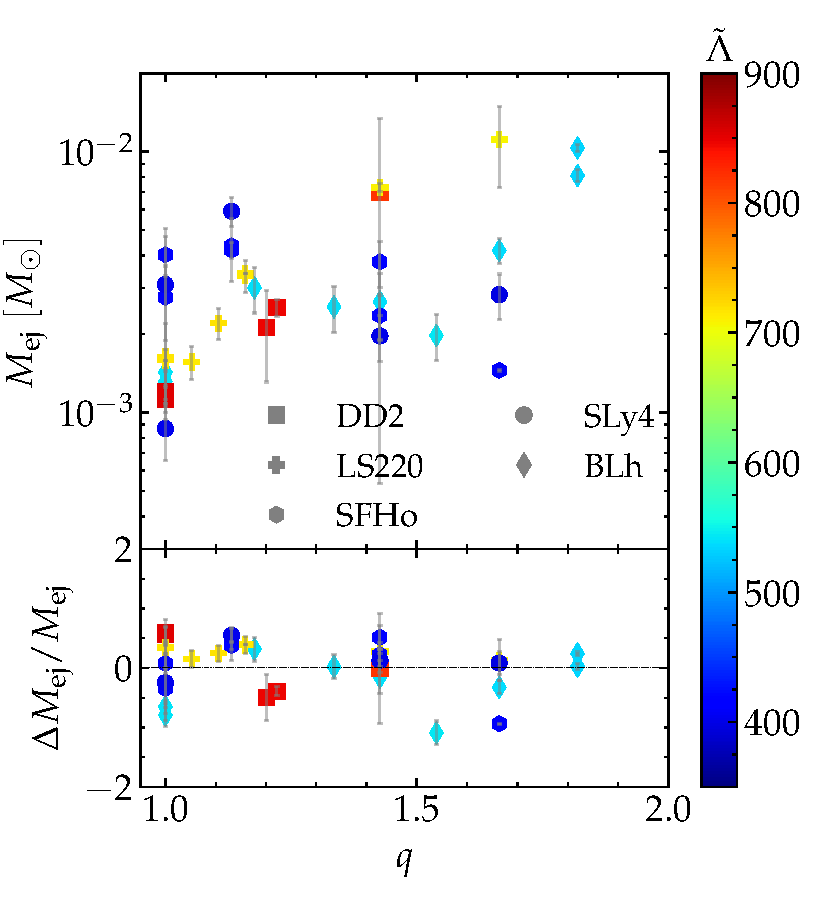
\includegraphics[width=0.49\textwidth]{statistics/ej_q_mej_our_poly22_cc.pdf}
    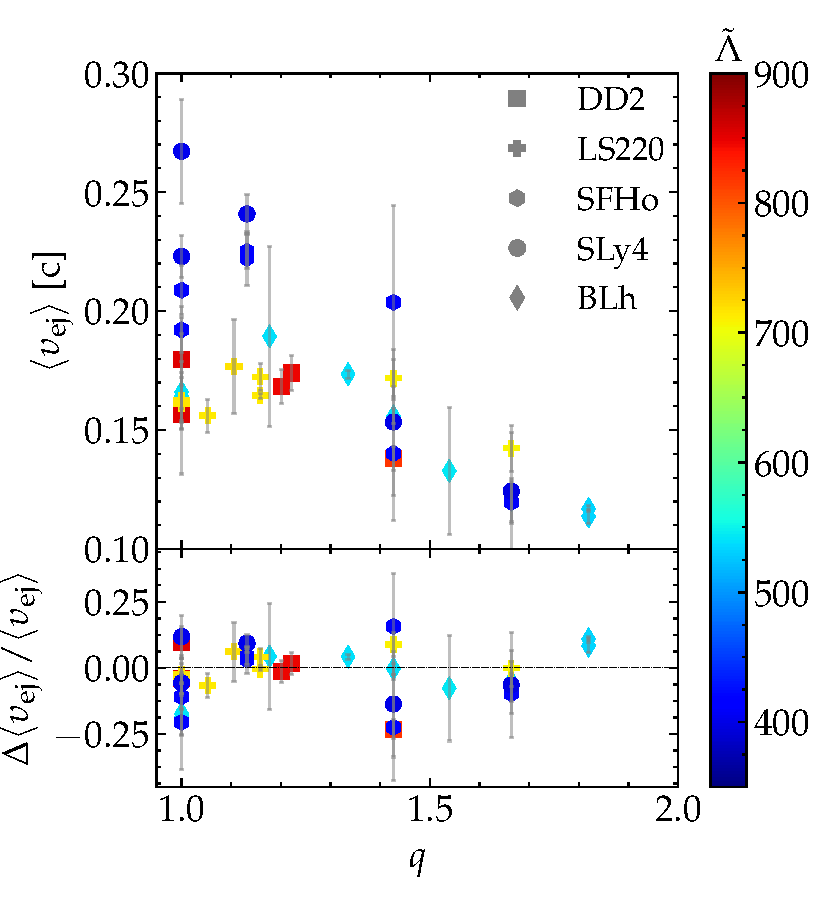
\includegraphics[width=0.49\textwidth]{statistics/ej_q_vej_our_poly22_cc.pdf}
    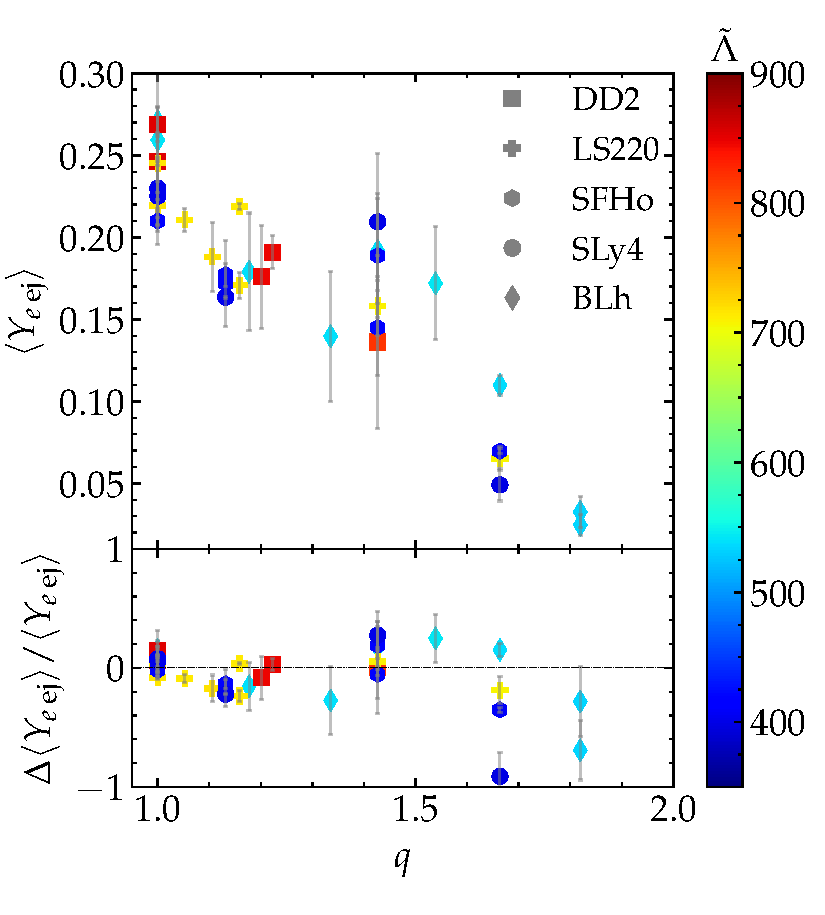
\includegraphics[width=0.49\textwidth]{statistics/ej_q_yeej_our_poly22_cc.pdf}
    \caption{
        Mass, mass-averaged velocity and electron fraction for \ac{DE} 
        from our simulation as functions of binary parameters $q$ and $\tilde{\Lambda}$, 
        on the \textit{first}, \textit{second} and \textit{third} \textit{panels} 
        respectively. 
        %
        In each panel, the lower suplot shows the relative difference 
        between the data and values inferred from the polynomial fitting 
        formula (see the text). 
        %
        (Adapted from \citet{Nedora:2020pak})
%        Dynamical ejecta properties as a function of mass ratio
%        and reduced tidal parameter. The dependency on the latter is
%        color coded. From left to right the main panels show the total
%        mass, the mass-averaged velocity and the electron fraction.
%        The bottom panels show the relative difference between the data
%        and the fit polynomial fit discussed in the text.
%        (Adapted from \citet{Nedora:2020pak})
        %\red{Is not referenced in velocity and Ye sections!}
        %\red{but referenced in the afterglow section}
    }
    \label{fig:ejecta:dyn:dsfits}
\end{figure*}
%
Comparing the ejecta properties between simulations with and 
without subgrid turbilence (See Tab.~\ref{tab:sim}) we observe 
that the effect of subgrid turbulence on the dynamical 
ejecta properties is rather week and comparable to the effects 
of finite grid discretization 
\citep{Bernuzzi:2020txg,Radice:2020ids}.

In Fig.~\ref{fig:ejecta:dyn:dsfits} we show the ejecta mass, velocity and 
electron fraction as a function of binary parameters: \mr{}, $q$, and 
reduced tidal deformability, $\tilde{\Lambda}$, for our models. 
The plot shows that while there is a large degree of scatter, certain 
overall trends can be deduced, and a relation between the ejecta and binary 
parameters can be constructed. 
%
In order to examine these relations in more details we enlarge the sample 
of simulations by collecting the published sets of \ac{BNS} merger models.
%
%%
%A specific goal of our analysis is the comparison with previous studies 
%of \ac{DE}, in particular with \citet{Radice:2018pdn}, where the same 
%simulation setup was used, but the neutrino reabsorption was not included.
%
%% -------------------
%% --- data available
\begin{sidewaystable}
%\begin{table*}[t]
    \caption{
        Characteristics of the collected sets of \ac{BNS} models. 
        The first column contains the sources from which the data was taken, 
        and the last column lists the names of the datasets that we define based on 
        the physics setup of simulations, specifically, neutrino treatment, that 
        is listed in the 3rd column. The second contains the information on the 
        \ac{EOS} which is either microphysical or piecewise polytropic (PWP).  
        Other columns state the availability of a certain binary and ejecta parameter. 
        The black crosses indicate that the data is not available, and thus, the corresponding 
        models were not used in the related analysis. 
%        Datasets with the dynamical ejecta data and disk masses
%        employed in this work. The available data is shown in the columns
%        starting from the fourth, that contain: gravitational mass of the binary, baryonic mass of
%        the binary, reduced tidal parameter, ejecta mass, ejecta
%        velocity, ejecta electron fraction, disk/torus mass. EOS are
%        either microphysical or piecewise polytropic (PWP). Neutrino
%        schemes are: leakage, leakage + M0 or M1 for free streaming
%        neutrinos, or M1. 
%        The compiled data are available online at \citep{vsevolod_nedora_2020_4283517}.
        (Adapted from \citet{Nedora:2020qtd})
    }
    \label{tab:data}
    \begin{tabular}{ccccccccccc}
        \hline\hline
        Ref.  & EOS  & Neutrinos & $M$  & $M_b$  & $\tilde{\Lambda}$ & $M_{\rm ej}$ & $\upsilon_{\rm ej}$ & $Y_e$  & $M_{\rm disk}$ & Dataset
        \\ \hline \hline
        \multicolumn{1}{c|}{\citep{Perego:2019adq}}     & \multicolumn{1}{c|}{Micro} & Leak+M0    & \cmark & \cmark & \cmark & \cmark & \cmark  & \cmark & \cmark &  \DSrefset{} \& \DSheatcool \\
        \multicolumn{1}{c|}{\citep{Nedora:2019jhl}}     & \multicolumn{1}{c|}{Micro} & Leak+M0    & \cmark & \cmark & \cmark  & \cmark  & \cmark & \cmark & \cmark  & \DSrefset{} \& \DSheatcool  \\
        \multicolumn{1}{c|}{\citep{Bernuzzi:2020txg}}   & \multicolumn{1}{c|}{Micro} & Leak+M0    & \cmark & \cmark & \cmark & \cmark & \cmark & \cmark & \cmark & \DSrefset{} \& \DSheatcool   \\
        \multicolumn{1}{c|}{\citep{Nedora:2020pak}}        & \multicolumn{1}{c|}{Micro} &   Leak+M0   & \cmark & \cmark & \cmark & \cmark & \cmark & \cmark & \cmark   & \DSrefset{} \& \DSheatcool   \\
        \hline
        \multicolumn{1}{c|}{\citep{Vincent:2019kor}}    & \multicolumn{1}{c|}{Micro}  &  M1  & \cmark & \cmark & \cmark & \cmark & \cmark  & \cmark & \xmark   &  \DSheatcool{} \\
        \multicolumn{1}{c|}{\citep{Sekiguchi:2015dma}}  & \multicolumn{1}{c|}{Micro} &  Leak+M1   & \cmark & \xmark & \xmark  & \cmark & \xmark & \cmark & \xmark &  \DSheatcool \\
        \multicolumn{1}{c|}{\citep{Sekiguchi:2016bjd}}  & \multicolumn{1}{c|}{Micro} &  Leak+M1   & \cmark & \xmark & \xmark & \cmark & \cmark & \cmark & \cmark & \DSheatcool \\
        \multicolumn{1}{c|}{\citep{Radice:2018pdn}~(M0)} & \multicolumn{1}{c|}{Micro} & Leak+M0    & \cmark & \cmark & \cmark & \cmark & \cmark & \cmark & \cmark  &  \DSheatcool   \\
        \hline
        \multicolumn{1}{c|}{\citep{Lehner:2016lxy}}     & \multicolumn{1}{c|}{Micro} & Leak    & \cmark & \cmark & \xmark & \cmark & \cmark & \xmark & \xmark   &  \DScool \\
        \multicolumn{1}{c|}{\citep{Radice:2018pdn}~(LK)} & \multicolumn{1}{c|}{Micro} & Leak    & \cmark & \cmark & \cmark & \cmark & \cmark & \cmark & \cmark  & \DScool   \\
        \hline
        \multicolumn{1}{c|}{\citep{Kiuchi:2019lls}}     & \multicolumn{1}{c|}{PWP}   &  -    & \cmark & \cmark & \cmark & \cmark & \xmark  & \xmark & \cmark    & \DSnone \\
        \multicolumn{1}{c|}{\citep{Dietrich:2016hky}}   & \multicolumn{1}{c|}{PWP}  &  -     & \cmark & \cmark & \cmark & \cmark & \cmark  & \xmark & \cmark  &  \DSnone \\
        \multicolumn{1}{c|}{\citep{Dietrich:2016hky}}   & \multicolumn{1}{c|}{PWP}  &   -    & \cmark & \cmark & \cmark & \cmark & \cmark & \xmark & \cmark  & \DSnone \\
        \multicolumn{1}{c|}{\citep{Hotokezaka:2012ze}}  & \multicolumn{1}{c|}{PWP}  &    -   & \cmark & \xmark & \xmark & \cmark & \cmark & \xmark & \xmark  &  \DSnone \\
        \multicolumn{1}{c|}{\citep{Bauswein:2013yna}}   & \multicolumn{1}{c|}{Micro}&  - & \cmark & \xmark & \xmark & \cmark & \cmark & \xmark & \xmark  &  \DSnone \\
        \hline\hline
    \end{tabular}
%\end{table*}
\end{sidewaystable}

%% -------------------
%
The datasets used for the analysis are summarized in Tab.~\ref{tab:data}.
We group them with respect to the employed neutrino treatment:

\begin{itemize}
    %% ---
    \item \DSheatcool{} comprises a set of models with neutrino emission 
    and absorption and microphysical \ac{EOS}. It includes 
    $8$ models with leakage+M0 of \citet{Radice:2018pdn} and models 
    of \citet{Sekiguchi:2015dma,Sekiguchi:2016bjd,Vincent:2019kor}
    in which a leakage+M1 scheme or a M1 gray scheme are employed for the neutrino transport. 
    Models reported in these studies span 
    $q\in[1, 1.30]$, 
    $\tilde{\Lambda}\in[340, 1437]$, 
    $M_{\rm tot}\in[2.52,2.88]$, 
    and $M_{\rm chirp}\in[1.10,1.25]$.
    %% ---
    \item \DSrefset{} harbors our models. 
    %    with the same physical setup as 
    %    those models with leakage+M0 of \citet{Radice:2018pdn}, that are 
    %    part of the \DSheatcool{}. However, these models, presented in 
    %    \citet{Perego:2019adq,Nedora:2019jhl,Bernuzzi:2020txg,Nedora:2020pak}, 
    %    and disucssed in Ch.~\ref{ch:bns_sims}, 
    For the reason that they are uniform in terms of the 
    numerical setup, code and physics and have fixed chirp mass 
    we group them into a separate, reference dataset. 
    The models of this set span $q\in[1, 1.82]$, 
    $\tilde{\Lambda}\in[400, 850]$, 
    $M_{\rm tot}\in[2.73,2.88]$ with 
    the chirp mass $M_{\rm chirp}=1.19$.
    %% ---
    \item \DScool{} comprises models with leakage scheme as neutrino treatment and 
    microphysical \ac{EOS}. The dataset includes a subset of models from 
    \citet{Radice:2018pdn} %($35$ runs denoted as LK),
    and the set of models from \citet{Lehner:2016lxy}.
    The models in this dataset span $q\in[1, 1.31]$, 
    $\tilde{\Lambda}\in[116, 1688]$, 
    $M_{\rm tot}\in[2.40,3.42]$, 
    and $M_{\rm chirp}\in[1.04,1.49]$.
    %% ---
    \item \DSnone{} is composed of models with piecewise-polytropic \acp{EOS} 
    \citet{Hotokezaka:2012ze,Dietrich:2015iva,Dietrich:2016hky,
        Kiuchi:2019lls,Bauswein:2013yna},
    in which temperature effects are approximated by a
    gamma-law pressure contribution, while
    composition and weak effects are neglected.
    The models in this dataset span 
    $q\in[1, 2.06]$, 
    $\tilde{\Lambda}\in[50, 3196]$, 
    $M_{\rm tot}\in[2.4,4.0]$, 
    and $M_{\rm chirp}\in[1.04,1.74]$.
\end{itemize}

%% --- Overal dataseamble
In total $324$ \ac{NR} models are collected. In cases where $\tilde{\Lambda}$ 
is not available, we compute it by solving \ac{TOV} equations 
for the corresponding gravitational masses and \acp{EOS}.
% 
For a subset of models with polytropic \acp{EOS} of \citet{Bauswein:2013jpa}
and \citet{Kiuchi:2019lls}, however, the \ac{EOS} data are not available and 
the $\tilde{\Lambda}$ cannot be estimated. We exclude these models from the 
statistical analysis. Overall, out of $324$, we consider $271$ models for which 
the required binary data is available/computed. For all $271$ models the ejecta 
mass, $\amd$, is present. The average velocity, $\avd$, is available for only $246$ 
models, as a subset of models from \citet{Kiuchi:2019lls} does not contain this 
information. The electron fraction is found for $99$ models, as we exclude the 
subset of models of \citet{Lehner:2016lxy} with leakage scheme for which this 
data is not given. 
%The \ac{RMS} half-opening angle around the orbital plane, 
%$\athetarms$, of the ejecta is present for $76$ models and the mass of the disk, 
%$M_{\rm disk}$, is given for $119$ models.

\begin{figure*}[t!]
    \centering 
    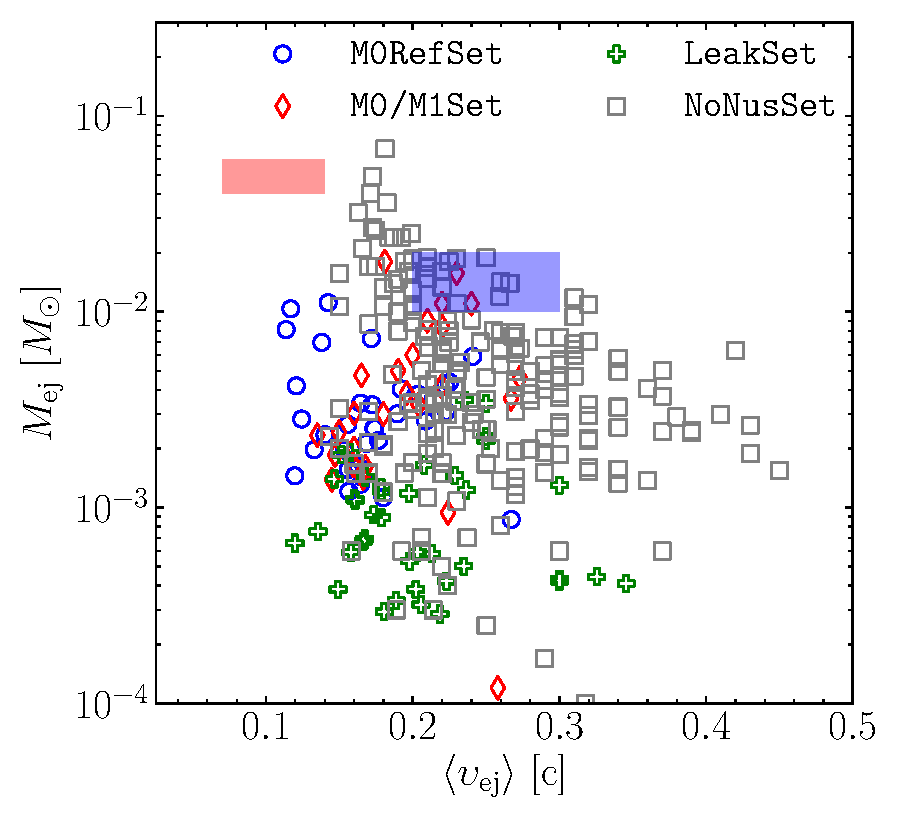
\includegraphics[width=0.45\textwidth]{statistics/ej_mej_vej_groups.pdf}
    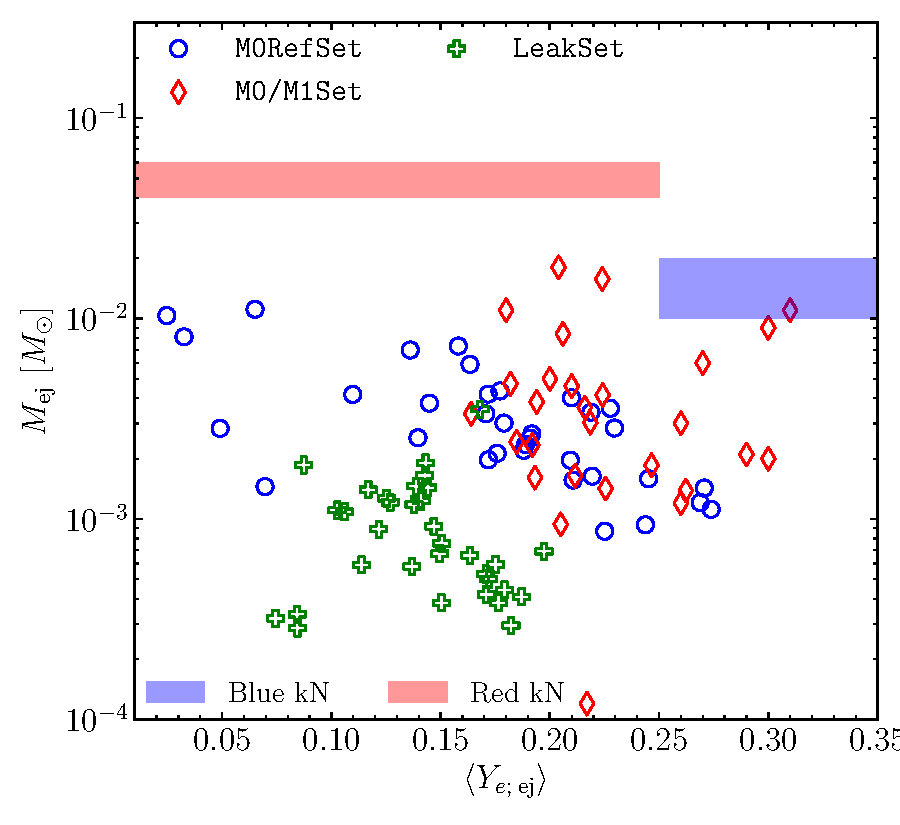
\includegraphics[width=0.45\textwidth]{statistics/ej_mej_yeej_groups.pdf}
    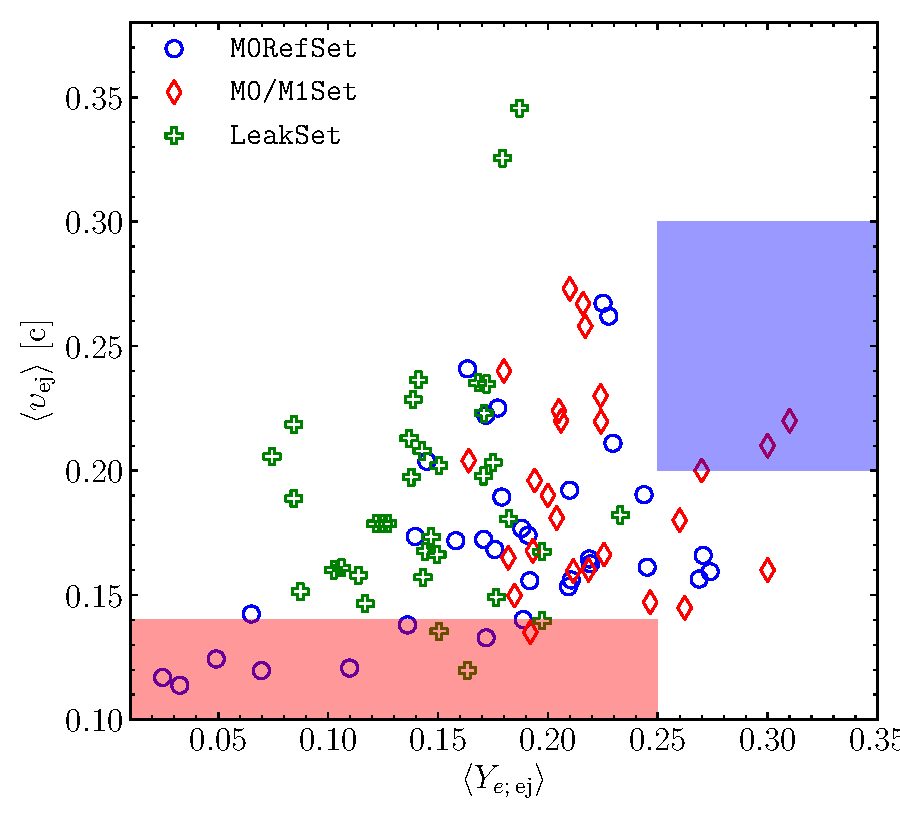
\includegraphics[width=0.45\textwidth]{statistics/ej_vej_yeej_groups.pdf}
    \caption{
        Properties of \ac{DE} for all datasets (Tab.~\ref{tab:data}), 
        including total ejecta mass, $M_{\rm ej}$, mass-averaged electron 
        fraction, $\langle Y_{\rm e;ej}$, and velocity 
        $\lambda\upsilon_{\rm ej}\rangle$. 
        The colored patches represent ranges inferred from \AT{} 
        \ac{kN} models \citep{Villar:2017wcc,Siegel:2019mlp}  
        (see Ch.~\ref{ch:kilonova} for the \ac{kN} discussion). 
        (Adapted from \citet{Nedora:2020qtd}). 
%        Summary of dynamical ejecta properties used in this work.
%        Blue circles represent models of \DSrefset{}, 
%        red diamonds stands for models from \DSheatcool{}, 
%        green crosses are models from \DScool{}
%        and gray squares stand for models from \DSnone{}, 
%        We show for comparison the two-component fit to AT2017gfo as
%        colored patches from \cite{Villar:2017wcc,Siegel:2019mlp}.
%        (Adapted from \citet{Nedora:2020qtd})
    }
    \label{fig:ejecta:dyn:ds}
\end{figure*}

The collected data is shown in Fig.~\ref{fig:ejecta:dyn:ds}. We note that the overall properties of the 
ejecta are similar between the \DSrefset{} and \DSheatcool{}. This is expected, as these 
datasets include similar, albeit not the same, physics, regarding \ac{EOS} and neutrino treatment.
%
The important exceptions are the high \mr{} models of \DSrefset{}, 
that undergo \ac{PC}. The \ac{DE} ejecta from these models is of tidal origin only. 
%\citep{Bernuzzi:2020txg}.
%
Comparing the properties of datasets with and without neutrino reabsorption, we observed 
that the the inclusion of this effect leads to the \ac{DE} of higher mass, in addition to 
the epxected increase in average electron fraction. This is especially noticeable when 
comparing models of \DSrefset{} and a subset of \citet{Radice:2018pdn} with leakage scheme only.


In Appendix \ref{app:coefs} we report the detailed statistical analysis, where we examine the 
change in mean values of ejecta properties between different datasets and fit the 
data with different fitting formelae found in literature, as well as, applying simple 
polynomials of $q$ and $\tilde{\Lambda}$ of second order,
$P_2^1(\tilde{\Lambda})$ and $P_2^2(q,\tilde{\Lambda})$, respectively. 
The results of this analysis are the following. 

%% --- Mej
For the ejecta mass we observe that the inclusion of \mr{} is required 
to capture the leading trends in data and the simple polynomial, 
$P_2^2(q,\tilde{\Lambda})$, shows a comparatively good statistical performance.
%\gray{We recomment the calibration based on the models with }
%
The statistical analysis also suggests that the $\amd$ depends 
sensibly on the physics input of the simulations: neutrino scheme and \ac{EOS} treatment.
%
The magnitude of systematic uncertainties in data, however, reduces the ability of any 
fitting formulae to identify and quantitatively capture leading trends.
%

%% --- vej
%We find that in our set of models, there is a correlation of $\avd$ with the 
%tidal parameter $\tilde{\Lambda}$: the higher the $\tilde{\Lambda}$ the lower 
%the $\avd$. This can be understood from the tidal/shocked components of the 
%\ac{DE} (see Sec.~\ref{sec:intro:merg_pmerg}) \red{BROKEN REF?}.
Considering the mass-averaged ejecta velocity, $\avd$, of the \DSrefset{}, we 
find that it is in overall agreement with the dataset with neutrino leackage scheme 
of \citet{Radice:2018pdn}, and ranges from $0.11\, c$ to $0.27\, c$. However, while in 
that study there was no apparent correlation observed between the velocity and binary 
parameters, upon visual inspection we find that in models of \DSrefset{} the $\avd$ 
is correlated with $\tilde{\Lambda}$, as shown in Fig~\ref{fig:ejecta:dyn:dsfits}.
This might be attributed to the fact that the \DSrefset{} encompass models with fixed 
chirp mass. 
%
The best fitting formula to the $\avd$, among considered, is $P_2^2(q,\tilde\Lambda)$, 
that appears to be able to capture the leading trends in data. 
%For its calibration, the dataset with the most advanced physics is 
%recommended, \DSheatcool{} \& \DSrefset{}.
%
The ejecta velocity shows a strong dependency on the neutrino treatment 
and binary parameters, specifically, the \mr{}.

%% --- Yeej 
Considering the average value of mass-averaged electron fraction, $\ayd$, we find 
that when only models of \DSrefset{} are considered, $\ayd$ varies 
between $0.03$, found in very high \mr{} binaries, that produce cold, low-$Y_e$,
tidal ejecta, and $0.27$ in $q\sim1$  % \citep{Bernuzzi:2020tgt}
binaries, where the contribution from the shocked component is significant 
(see also Fig.~\ref{fig:ejecta:dyn:dsfits}). 
%
Naturally, datasets that include the effects of neutrino absorption display 
on average higher $\ayd$. 
%
Here we only consider the polynomials as fitting formulae. 
The analysis suggests that $P_2^2(q,\tilde\Lambda)$ is the best fitting one, 
as it is able to reproduce both the low-$Y_e$ and high-$Y_e$ models of 
\DSheatcool{} and \DSrefset{}.
%Comparing the values of $\ayd$ from datasets and predicted by fitting formulae in 
%we find that for all datasets, the $P_2^2(q,\tilde\Lambda)$ is able to 
%reproduce both the low-$Y_e$ and high-$Y_e$ models of 
%\DSheatcool{} and \DSrefset{}.

%% --- theta_RMS
%% THETA RMS [3 pandles REFSET]
\begin{figure*}[t]
    \centering 
    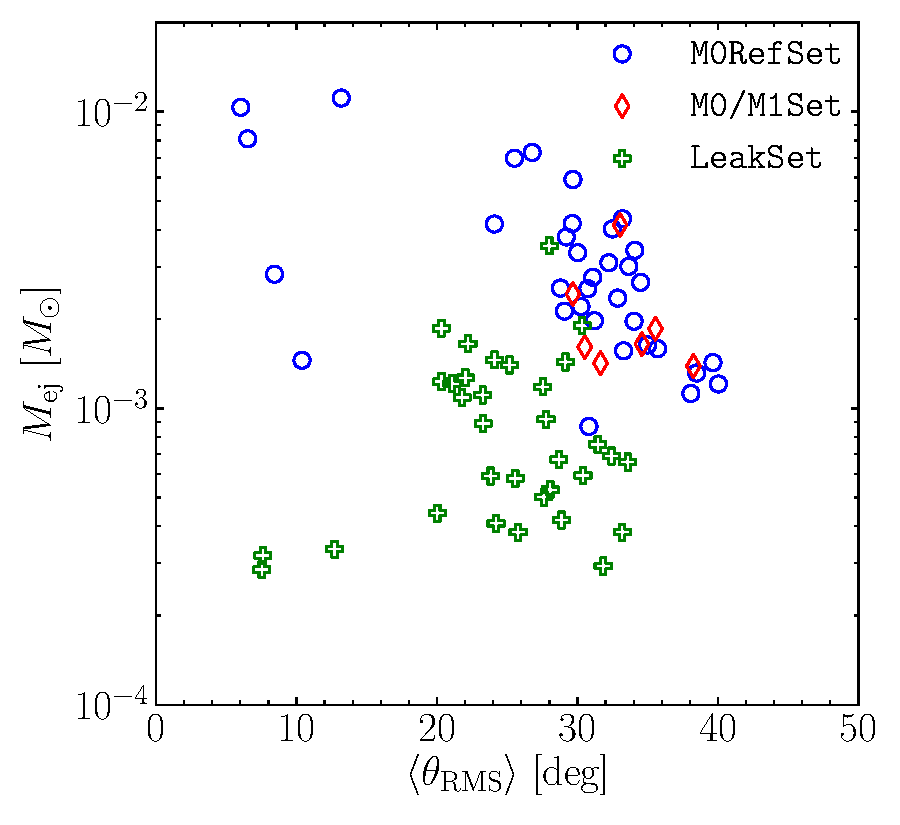
\includegraphics[width=0.45\textwidth]{statistics/ej_mej_theta_groups.pdf}
    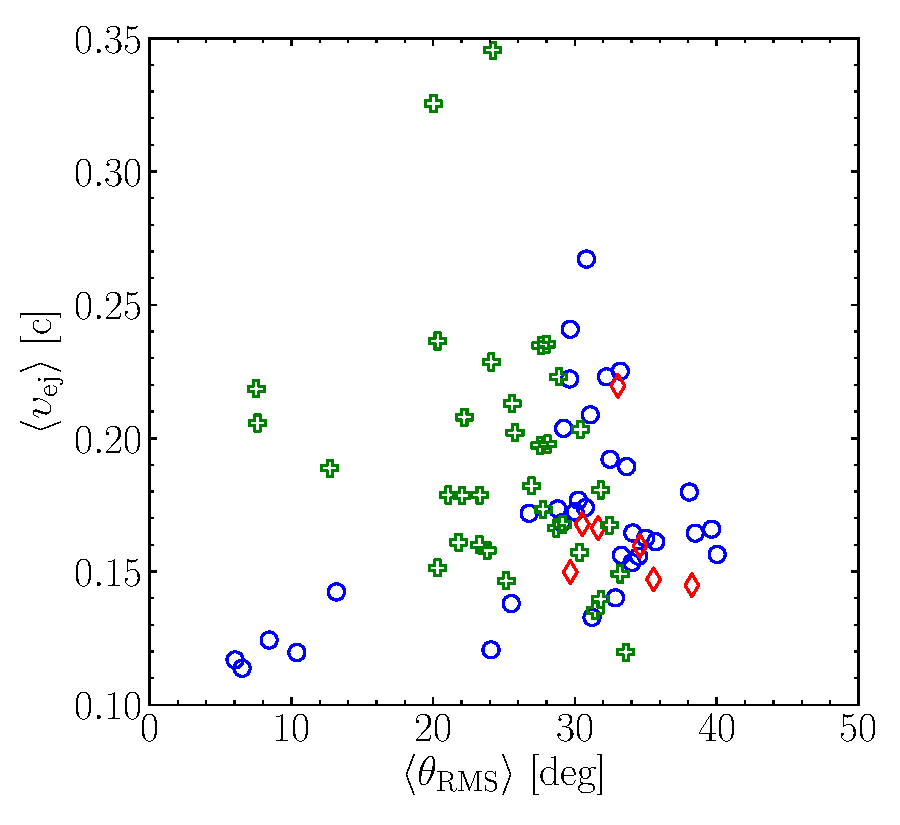
\includegraphics[width=0.45\textwidth]{statistics/ej_vej_theta_groups.pdf}
    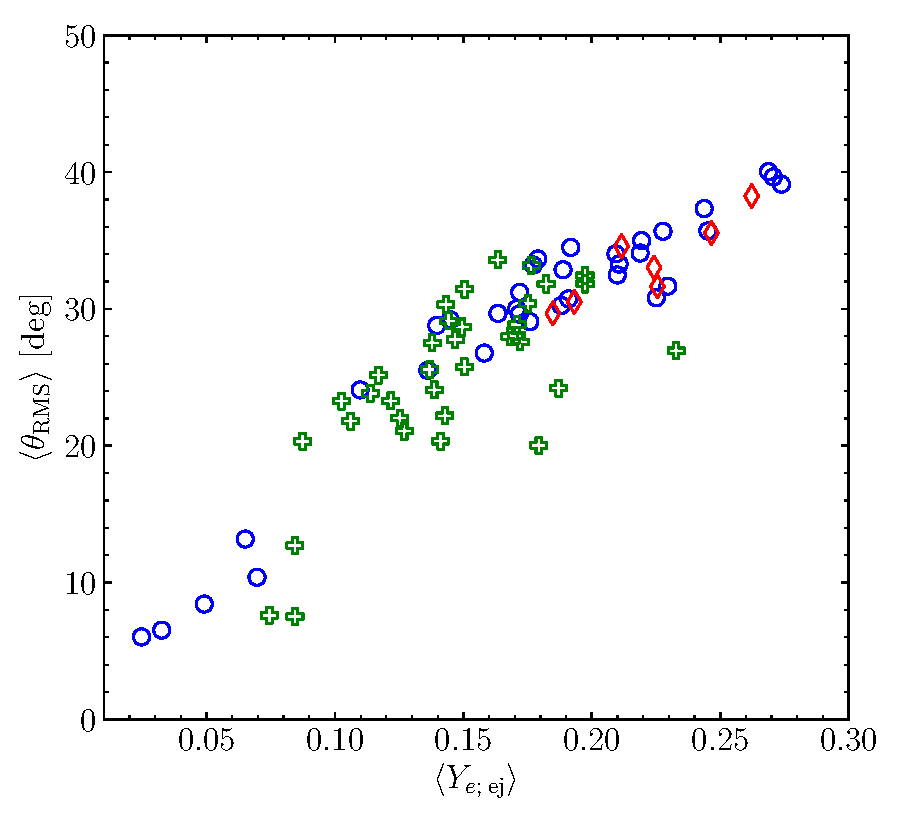
\includegraphics[width=0.45\textwidth]{statistics/ej_theta_yeej_groups.pdf}
    \caption{
        Same as Fig.~\ref{fig:ejecta:dyn:ds}, but including also the 
        mass-averaged \ac{RMS} half-opening angle about the orbital plane of the 
        \ac{DE} distribution, $\athetarms$. The plotted 
        data is limited to datasets in which this quantity is available. 
        %
        %The last panel shows a clear correlation between $\theta_{\rm RMS}$ and $\ayd$. 
        (Adapted from \citet{Nedora:2020qtd}).
%        Properties of \ac{DE} for all datasets (Tab.~\ref{tab:data}), 
%        including total ejecta mass, $M_{\rm ej}$, mass-averaged electron 
%        fraction, $\langle Y_{\rm e;ej}$, and velocity 
%        $\lambda\upsilon_{\rm ej}\rangle$. 
%        Relations between the ejecta $\theta_{\rm RMS}$ and other parameters of the dynamical
%        ejecta: mass, $\amd$, velocity, $\avd$, and electron fraction $\ayd$ for models from
%        \DSrefset{} and \cite{Radice:2018pdn} from \DScool{} and \DSheatcool{}.
%        Plots show that models with neutrino absorption have
%        higher $\amd$ and larger $\theta_{\rm RMS}$ as well as 
%        a clear correlation between $\theta_{\rm RMS}$ and $\ayd$.
%        (Adapted from \citet{Nedora:2020qtd})
    }
    \label{fig:ejecta:dynej_thetarms}
\end{figure*}

\begin{figure*}[t!]
    \centering 
    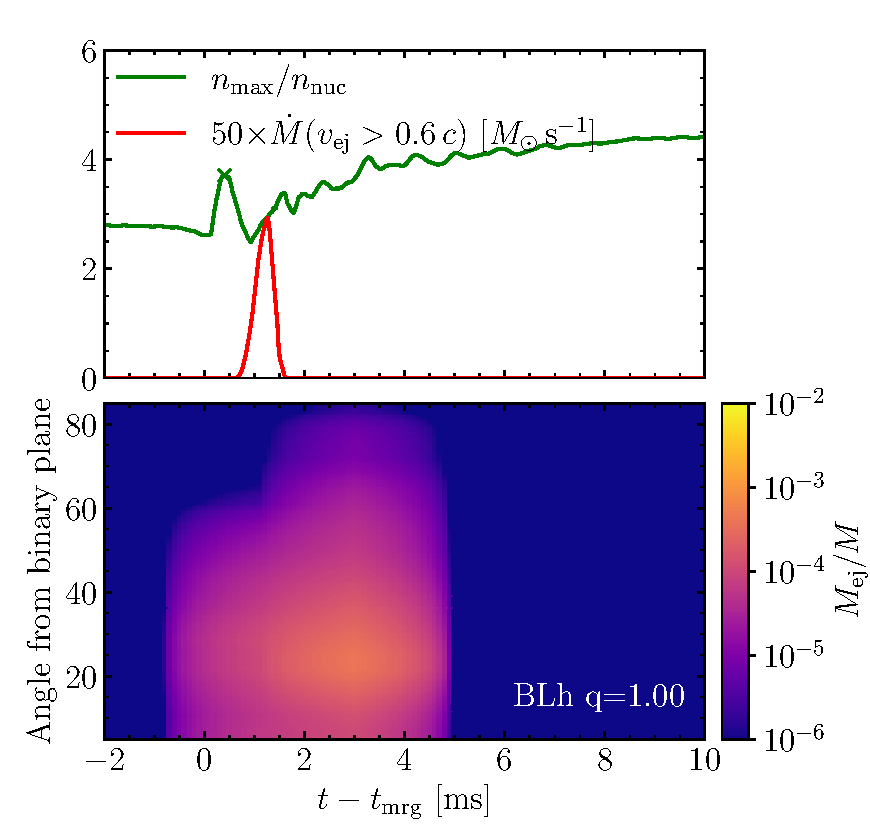
\includegraphics[width=0.49\textwidth]{ejecta_dyn/fast_ejecta/BLh_q100_LK_SR.pdf}
    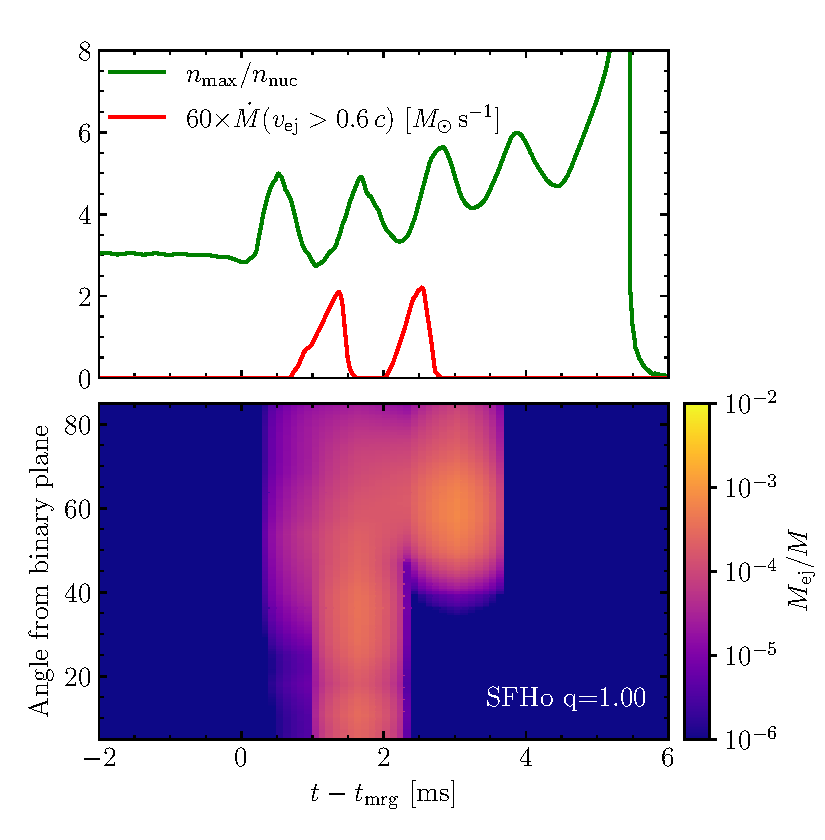
\includegraphics[width=0.49\textwidth]{ejecta_dyn/fast_ejecta/SFHo_q100_LK_SR.pdf}
    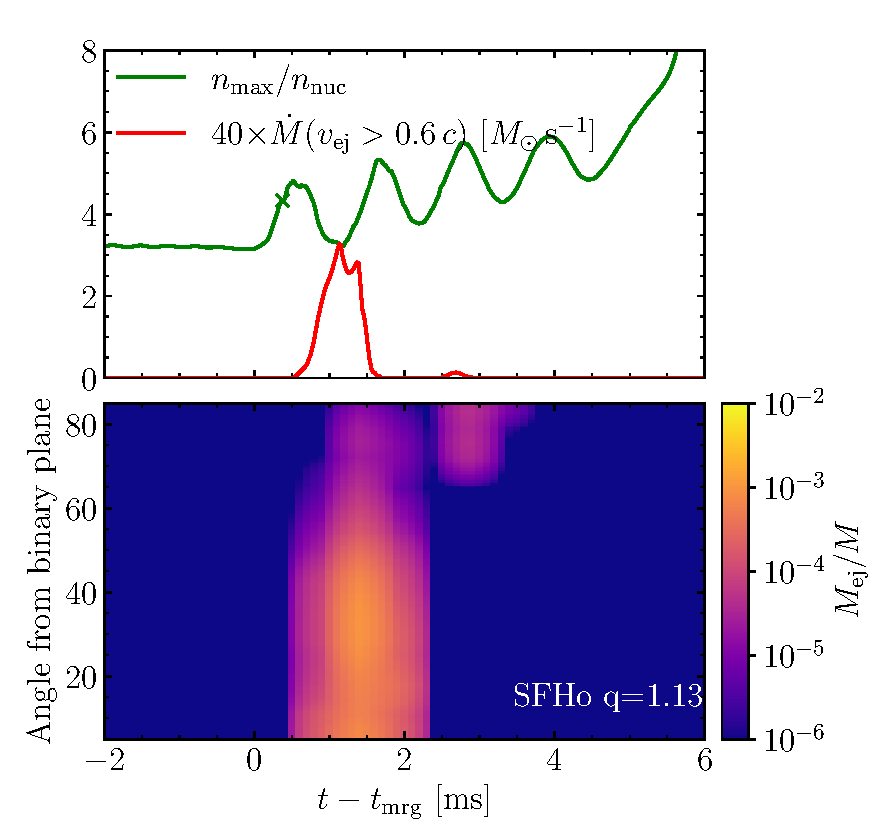
\includegraphics[width=0.49\textwidth]{ejecta_dyn/fast_ejecta/SFHo_q112_LK_SR.pdf}
    %% \includegraphics[width=0.49\textwidth]{./figs/scatter_lambda_ekej_vej06.pdf}
    %% \includegraphics[width=0.49\textwidth]{./figs/scatter_mej_vej06.pdf}
    %% \includegraphics[width=0.49\textwidth]{./figs/scatter_total_kinetic_energy.pdf}
    %%     \includegraphics[width=0.49\textwidth]{./figs/scatter_thetarms_vej06.pdf}
    %%     \includegraphics[width=0.49\textwidth]{figs/scatter_lightcurve_peaks_vs_lambda.pdf}
    \caption{
        Time evolution of the fast tail of \ac{DE}, $\dot{M}(\upsilon_{\rm ej}>0.6\,c)$, 
        alongside the time evolution of normalized central density $n_{\rm max}/n_{\rm nuc}$ 
        for three simulations, BLh $q=1.00$, SFHo $q=1.00$ and SFHo $q=1.13$, one per panel. 
        %
        The lower subpanel on each panel depicts the time evolution of the fast tail of 
        \ac{DE} angular distribution. 
        %% \vn{[Might be removed, if needed]}
        %        Ejection mechanism and properties of the fast tail of the ejecta shown for three simulations,
        %        with two \acp{EOS}: BLh and SFHo and two \mr{}s: $q=1.00$ and $q=1.22$.
        %        %% ---
        %        The upper panel in each plot shows the time evolution of the maximum density 
        %        in the simulation (green curves) and the mass flux of the ejecta with 
        %        asymptotic velocities exceeding $0.6c$ (red curve).
        %        %% --- 
        %        The bottom panel shows the mass histogram of the fast ejecta tail as a function 
        %        of time. 
        %% --- 
        In both panels the outflow rate and histograms are computed at a radius of 
        $R = 443$~km and shifted in time by 
        $R\langle\upsilon_{\rm fast}\rangle ^{-1}$, 
        $\langle\upsilon_{\rm fast}\rangle$ being the mass averaged velocity of 
        the fast tail at the radius $R$.
        %% --- 
        %        The plot shows that while in mist models the peak of the fast ejecta mass flux 
        %        coincides with the first core \bnc{}, in agreement with \cite{Radice:2018pdn}, 
        %        in the model with 
        %        
        %        The plot shows that most of the fast ejecta are generally produced at first core \bnc{} with a contribution from the second in models with soft \acp{EOS}.
        (Adapted from \citet{Nedora:2021eoj}). 
    } 
    \label{fig:ejecta_v06_mech}
\end{figure*}


%
The ejecta geometry has been shown to be very important for modeling \ac{EM} 
counterparts to mergers (see Chapter~\ref{ch:kilonova} and Chapter~\ref{ch:afterglow}). %\citep[\eg][]{Perego:2017wtu}. 
However, its statistical analysis is very non-trivial. 
Because of the limited data and for the sake of simplicity 
we consider the mass-averaged \ac{RMS} half-opening 
angle of the ejecta about the plane of the binary, $\athetarms$.
%% --- 
We introduce the $\athetarms$ in accordance with \citet{Radice:2018pdn}, assuming 
the axial symmetry and computing:
%
\begin{equation}
\athetarms = \frac{180}{\pi}\Bigg(\frac{\sum m_i \theta_i^2}{\sum m_i}\Bigg)^{1/2}\, ,
\end{equation}
%
where $\theta_i$ and $m_i$ are the angle (from the binary plane) and the mass of 
the element of ejecta respectively.
%
Unfortunately, this quantity is available only for the \DSrefset{} and for a subset 
of models of \citet{Radice:2018pdn}. 
% some of which are in \DScool{} and some are in \DSheatcool{} (see Tab~\ref{tab:data}). 
Hence, the statistical analysis is limited 
to a small sample of models. The dependency of the $\athetarms$ on other ejecta 
properties discussed before is shown in Fig.~\ref{fig:ejecta:dynej_thetarms}.
%
With respect to the models of \citet{Radice:2018pdn}, we observe that the models of the 
\DSrefset{} have overall larger $\athetarms$. This suggests that the inclusion of 
neutrino reabsorption leads to a more spherically distributed ejecta.
%
The third panel of Fig.~\ref{fig:ejecta:dynej_thetarms} shows a clear linear relation 
between the $\athetarms$ and $\ayd$, that can be attributed to the \mr{} dependency of 
ejecta properties observed before, that we extend as follows. 
Binaries with large \mr{} have ejecta of mostly tidal origin that 
is confined to the binary plane and characterized by low electron fraction. 
Meanwhile, binaries with $q\sim 1$ have ejecta of both tidal and shock origin that both 
more spread out and more processed by shocks and neutrino irradiation having, thus,
higher $\ayd$. 
%
Similar to the case of $\ayd$, we find that the \polql{} provides the best fit to the data.

Overall, we observe that the properties of \ac{DE} depend on \mr{} and 
\ac{EOS} softness that can be parameterized with $\tilde{\Lambda}$, and a simple 
polynomial in these two quantities show a comparable or better performance with 
resepct to other fitting formulae available in the literature. 
%
However, larger sample of ab-initio \ac{NR} simulations with complete physics and 
publicly available data is are required to refine these relations.

%We overview the overall properties of the dynamical ejecta in our simulations 
%in in the chapter \ref{ch:stat}, placing them alongside the other available data 
%in the literature.

%We can qualitatively asses the effects of neutrino heating by comparing the overall 
%properties of our models with those of \citet{Radice:2018pdn}, where the same 
%simulation setup and code were used but only neutrino leakage scheme was employed.
%%
%We perform this comparison and the comprehansive statitical analysis of the 
%ejecta properties in the chapter \ref{ch:stat}.
%
%Specifically, we observer, 
%Comparing out simulation data with other models available in the literature 
%(Sec.~\ref{sec:stat:ejecta}), we find that neutrino absorption leads to not only 
%an increase in average electron fraction but also to larger total ejected mass 
%and velocity. 
%The latter two would be crucial for the non-thermal, 
%kilonova afterglow (see Sec.\red{sec:KilonovaAfterglow}).
%%
%The mass averaged over the simulations from Tab.~\ref{tab:sim} is 
%$\overline{\amd} = (3.442 \pm 2.495)\times 10^{-3}\,M_{\odot}$ (where
%hereafter we report also the standard deviation), while the same
%quantity calculated for data of \citep{Radice:2018pdn} 
%is $\overline{\md} = (1.352\pm 1.250)\times 10^{-3}\,\Msun$.
%The mass-averaged terminal velocity of the dynamical ejecta 
%ranges between $0.1\,c$ and $0.3\,c$, and in a good agreement with 
%\citep{Radice:2018pdn}.
%The mass-averaged velocity, averaged over all the simulations, is 
%$\overline{\avd} = (0.172\pm0.038)\,{\text{c}}$.
%
%We find that in our set of models, there is a correlation of $\avd$ with the 
%tidal parameter $\tilde{\Lambda}$: the higher the $\tilde{\Lambda}$ the lower 
%the $\avd$. This can be understood from the tidal/shocked components of the 
%\ac{DE} (see Sec.~\ref{sec:intro:merg_pmerg}) \red{BROKEN REF?}.
%%
%We also find that the ejecta velocity, found in our simulations, 
%is recovered in \ac{NR} simulations with more advanced neutrino 
%treatment performed by other groups (see App.~\ref{sec:stat:vejstat}).
%
%From the plot we observe that the $\avd$ increases with $\tilde{\Lambda}$. This can 
%be attributed to the fact that the \ac{DE} in mergers with $q\sim1$ is dominated by the 
%shocked component and that the shocked component has on average higher velocities when 
%the \acp{NS} of lower radii (with larger $\tilde{\Lambda}$) collide.
%
%that tells in mergers of binaries with $q=1.00$, the shocked component of the ejecta 
%is the dominant. The strength of shocks increases as the \acp{NS} become more compact 
%(with decreasing $\tilde{\Lambda}$) and hence collide at higher velocities~\footnote{Note that in the definition of prompt collapse we adopted, there is no shocked ejecta.}.
%%% ---
%For binaries with high mass ration, however, the tidal component of the \ac{DE} is dominant. 
%The velocity of the latter also is smaller for larger $\tilde{\Lambda}$, as stars collide 
%at slower velocities due to their larger radii. 
%%% ---
%In our models, the mass-averaged electron fraction, $\ayd$, 
%lies the range $(0.1, 0.3)$.
%with an averaged value among all models $\overline{\ayd} = 0.175 \pm 0.063$.
%Notably, the \citet{Radice:2018pdn} reported a more narrow range, $(0.1, 0.2)$.
%This is a clear effect of the neutrino absorption included in our models, that elevates 
%the everal electron fraction of the \ac{DE} as it is being irradiated by neutrinos 
%during the merger.
%Notably, the $\ayd$ of our models is close to those obtained with M1 
%scheme of \citet{Sekiguchi:2016bjd} and \citet{Vincent:2019kor}.
%%% ---
%The angular distribution of the \ac{DE} is found to depend 
%on the neutrino treatment. Specifically, the inclusion of 
%neutrino reabsorption leads to a more spherically distributed ejecta
%(see App.~\ref{sec:stat:thetarms}).
%%%%---
%The effect of subgrid turbulence on the dynamical ejecta properties however,
%found rather week and comparable to the effects of finite grid discretization 
%\citep{Bernuzzi:2020txg,Radice:2020ids}.
%
%Overall, we observe that the properties of the \ac{DE} depend on the \mr{} and 
%\ac{EOS} softness that can be parameterized with $\tilde{\Lambda}$, as 
%%
%\begin{align}\label{eq:polyfit2}
%P_2 ^1(\tilde{\Lambda}) &= b_0 + b_1\tilde\Lambda + b_2 \tilde\Lambda^2, \\\label{eq:polyfit22}
%P_2 ^2(q,\tilde\Lambda) &= b_0 + b_1q + b_2\tilde\Lambda + b_3q ^2 +  b_4 q \tilde\Lambda + b_5\tilde\Lambda^2 \, .
%\end{align}
%%
%The result of a fitting ejecta parameters with the polynomial of these two quantities 
%are shown in bottom panels of Fig.~\ref{fig:ejecta:dyn:dsfits}.
%%
%This assertion is supported by a more thorough analysis of the ejecta 
%properties and disk mass, discussed in Appendix.~\ref{ch:stat}, 
%and thus we refer to these formulae as ``best fitting formulae''.
%%
%A larger sample of ab-initio simulations with complete physics and 
%publicly available data are required to refine these relations.






\subsection{Fast tail of the dynamical ejecta} \label{sec:bns_sims:fast_de}

%\red{\bnc{} is introduced in intro, Sec.~\ref{sec:intro:merg_pmerg}}

In order to analyze the low mass, very fast compoent of the \ac{DE}, we 
choose the furthest extraction sphere from the remnant, at 
$R = 443\,$km.  %300G/c^2M_{\odot}
%In this section we discuss the ejecta properties that are extracted at 
%coordinate radius of $R=300G/c^2M_{\odot}\approxeq443\,$km from the center.
This assures that the ejecta had the longest evolution 
within the simulation domain. In addition, this allows for a consistent
comparisons with the results of \citet{Radice:2018pdn}.
%
%We also limit the discussion to the simulations performed at a standard resolution
%(ee Sec.~\ref{sec:bns_sims:setup}). Several available simulations that 
%were performed at higher resolution are used to asses the errors.
Following the authors, we define the fast ejecta component (tail) 
as the ejecta with $\upsilon_{\infty}\geq0.6\,c$.

We find the non-negligible amount of fast ejecta in all our simulations 
except for those with very stiff \acp{EOS} and high \mr{}s. 
%We find that not all the simulation show the presence of the fast ejecta tail.
%For instance, the fast ejecta component is absent in simulations with stiff \ac{EOS} 
%and relatively high \mr{}, 
%$q=M_1/M_2\geq1$ where $M_1$ and $M_2$ are the gravitational masses 
%at infinity of the primary and secondary \acp{NS} respectively.
The \ac{DE} velocity distribution from these models shows a sharp cut-off at ${\leq}0.5\,c$, 
that can be attributed to the fact that in these simulations, the \ac{DE} 
is primarily of tidal origin and displays on average lower velocities, 
that, in turn, is set mainly by the \acp{NS} velocities at 
the last orbit and the system escape velocity. 
%The absence of fast tail can be explained by the fact that 
%at large \mr{}s the ejecta are dominated by the tidal component, whose speed 
%is largely set by the \acp{NS} velocities at the last orbit and the system escape velocity.
%Moreover, models with large $q$ in our set undergo prompt collapse 
%with no core bounce \citep{Bernuzzi:2020txg}.

We show the mechanism that is responsible for producing most of the fast ejecta in 
Fig.~\ref{fig:ejecta_v06_mech}. We find that the 
ejection of mass with velocity $\upsilon>0.6\,c$ coincides with core \bnc{}s. 
This was previously noted bu \citet{Radice:2018pdn}.
Most of the ejecta originate at the first \bnc{} in models with moderately soft \acp{EOS} 
or large \mr{}s, \eg, BLh $q=1.00$ model. % the equal mass BLh \ac{EOS} model. 
Similar behaviour is observed in models with higher \mr{}s and softer \acp{EOS}. 
%\eg, SFHo \ac{EOS} model.
We also observe that in models with very soft \acp{EOS} 
(and small \mr{}s), \eg, SLy4* $q=1.00$ model, a strong influx of fast ejecta 
occurs during the second core \bnc{}.
%equal mass SLy4 \ac{EOS} model.
Notably, while the first-\bnc{} component is generally equatorial, 
the second-\bnc{} component is more polar. The possible explanation for this might 
include the increase in baryon pollution of the low latitude region around 
the \pmerg{} remnant.

%% --- Paragraph on the resolution effects and error bars 
In our sample of simulations, the resolution does not affect whether there is a fast tail 
of \ac{DE} or not, but it does affect its mass % $\md(\upsilon>0.6\, c)$. 
as we find that  
%$\md(\upsilon>0.6\, c)$ 
it changes by a factor of a few
between \texttt{SR} and \texttt{HR} simulations. 
A larger sample of simulations performed at high resolutions
is required to asses this uncertainty more quantitatively.
%% --- Properties of the fast tail: ejecta mass
%The mean value of the fast tail mass is
%\begin{equation}
%    \overline{\amd}(\upsilon>0.6\, c) = (2.36 \pm 3.89)\times 10^{-5}\,M_{\odot}\ ,
%\end{equation}
%where we also report the standard deviation.


%% --- Properties of the fast tail: velocity, electron fraction
Mass-averaged properties of the fast tail, such as velocity, electron fraction and 
angular distribution, appear robust with resolution, similarly to what was observed for 
the total dynamical ejecta (see Tab.~\ref{tab:sim}).
%% --- Table reference 
%We report the properties of fast tail in Tab.~\ref{tab:sims}.
%
We find that the mass-averaged velocity % , 
%$\vd(\upsilon>0.6\,c)$, 
is close to $0.6\,c$,
increasing with softness of the \ac{EOS}.
%
The mass-averaged electron
%, $\yd(\upsilon>0.6\, c)$ 
is generally above $0.25$, 
indicating that these ejecta were shock-heated and reprocessed by neutrinos. High 
average electron fraction implies that only weak \rproc{} \nuc{} would 
occur, producing elements up to the $2$nd $r$-process peak \citep{Lippuner:2015gwa} 
(see also Chapter~\ref{ch:nucleo}).


\begin{figure}%%[t]
    \centering 
    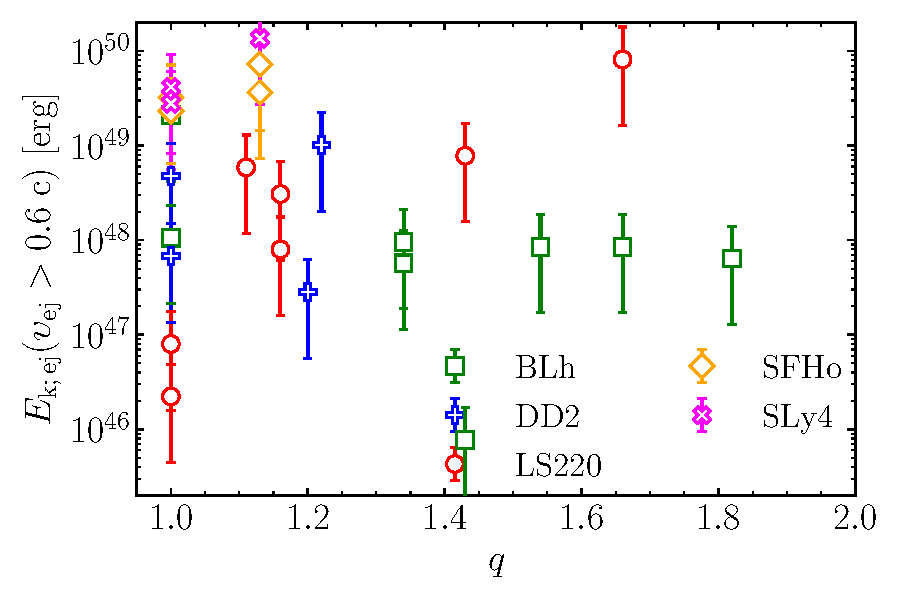
\includegraphics[width=0.50\textwidth]{ejecta_dyn/fast_ejecta/scatter_ekej_vej06.pdf}
    \hspace{-4mm}
    \includegraphics[width=0.50\textwidth]{ejecta_dyn/fast_ejecta/scatter_thetarms_vej06.pdf}
    %% \includegraphics[width=0.49\textwidth]{./figs/scatter_lambda_ekej_vej06.pdf}
    %% \includegraphics[width=0.49\textwidth]{./figs/scatter_mej_vej06.pdf}
    %% \includegraphics[width=0.49\textwidth]{./figs/scatter_total_kinetic_energy.pdf}
    %%     \includegraphics[width=0.49\textwidth]{./figs/scatter_thetarms_vej06.pdf}
    %%     \includegraphics[width=0.49\textwidth]{figs/scatter_lightcurve_peaks_vs_lambda.pdf}
    \caption{
        Total kinetic energy (\textit{left panel}) and \ac{RMS} half-opening angle 
        (\textit{right panel}) as a function of binary \mr{}, $q$, for the 
        of the fast tail of \ac{DE}. 
%        Properties of the fast tail of the dynamical ejecta:
%        total kinetic energy (\textit{top panel}) and 
%        half-\ac{RMS} angle around the binary plane (\textit{bottom panel})
%        from a selected set of simulations where this tail is present (see text).
%        We assume conservative uncertainties for the angle, $0.5$~deg, 
%        and half of the value for the kinetic energy. 
%        The top panel shows that only for some \acp{EOS} the 
%        total kinetic energy appear to depend on mass ration. Specifically, LS220m SFho and SLy4 \acp{EOS}.
%        The half-\ac{RMS} angle appears to depend more on \ac{EOS}, and to be overall larger for high-$q$ models.
        (Adapted from \citet{Nedora:2021eoj}). 
    } 
    \label{fig:ejecta_v06}
\end{figure}


%% --- Total energy discussion :: Fig.1 (top)
The total kinetic energy of the fast tail, $E_{\rm k}(\upsilon > 0.6\, c)$,
is shown in top panel of the Fig.~\ref{fig:ejecta_v06}.
Considering the resolution dependency of the ejecta mass and, less prominently, velocity, 
we set a conservative error bar of ${\sim}1$~order of magnitude.
%
The figure shows that the $E_{\rm k}(\upsilon > 0.6\, c)$ ranges between 
${\sim}10^{46}\,$erg, and ${\geq}10^{50}\,$erg, without showing 
strong dependency on the \ac{EOS}, even though models with very soft \acp{EOS} 
(\eg, SLy4 and SFHo) tend to display larger energies. 
%
The dependency on the \mr{} is more noticeable, especially for the 
SLy4, SFHo and LS220 \acp{EOS}, where for the latter, the 
$E_{\rm k}(\upsilon > 0.6\, c)$ 
increases by ${\sim3}\,$ orders of magnitude between $q=1$ and $q=1.7$. 
%Notably, for the BLh \ac{EOS} models, the $E_{\rm k}(\upsilon > 0.6\, c)$ 
%does not change with the \mr{}.

%% --- Angular distribution :: Fig.1 (bottom)
Considering the \ac{RMS} half-opening angle of the fast ejecta around the 
orbital plane (Fig.~\ref{fig:ejecta_v06}, left panel) we set the conservative 
error of $5$~degrees based on the comparison with higher resolution
simulations. 
%
%The figure allows to gauge which ejection mechanism dominates in 
%various simulation, as the ejecta angular distribution depends on it.
%
We observe that in models with stiff \acp{EOS}, \eg, DD2 \ac{EOS}, where the 
core first-\bnc{} ejection mechanism dominate, the fast ejecta tail is generally equatorial.
Meanwhile, in simulations with soft \acp{EOS} and high \mr{}s, the fast ejecta shows 
a more uniform angular distribution set by a combination of the core dynamics and 
finite temperature effects.% driving shocked material.

%% --- RESOLUTION DEPENDENCY 
%Comparing the total kinetic energy from simulations performed at standard and high resolutions we find that the $E_{\rm k;\, ej}$, is 
Assessing the resolution dependency of the ejecta parameters more quantitatively,
we report that for three representative models 
%for which the fast ejecta 
%were found in both the SR and high HR simulations, 
%% (with typical grid resolution $185$~m and $123$~m respectively) 
the $E_{\rm k \,; ej}(\upsilon_{\text{ej}} > 0.6)$ changes
by at least factor of a few
between \texttt{SR} and \texttt{HR}. 
The ejecta \ac{RMS} half-opening angle about the 
orbital plane is changing by utmost ${\sim}50\%$.



%% cp ~/GIT/GitHub/bns_em_analysis/scripts/figs/kinetic_energy_struct_models.pdf ~/GIT/GitHub/phd_thesis/v4/Figures/ejecta_dyn/fast_ejecta/
\begin{figure}%%[t]
    \centering 
    \includegraphics[width=0.55\textwidth]{ejecta_dyn/fast_ejecta/kinetic_energy_struct_models.pdf}
    \caption{
        Cumulative kinetic energy distribution (\textit{top panel}) for a set of 
        representative model and its angular dependence 
        for BLh $q=1.00$ model (\textit{bottom panel}). 
        %
        The green line corresponds to $\upsilon_{\rm ej}=0.6$. 
%        Cumulative kinetic energy distribution for a selected set of models (\textit{top panel}) 
%        and its angular distribution for a BLh $q=1.00$ model (\textit{bottom panel}).
%        %% Also shown as a solid black line is the slow quasi-spherical model of \cite{Mooley:2017enz}.
%        The vertical light green line marks the $\upsilon_{\text{ej}}=0.6$.
%        The top panel shows that equal mass models have a more extend high energy tail,
%        while the bottom panel shows that the angular distribution of the ejecta is not 
%        uniform.
        (Adapted from \citet{Nedora:2021eoj}). 
    } 
    \label{fig:ejecta_vel_hist}
\end{figure}


%% --- KINETIC ENERGY DISTRIBUTION :: Fig.2 <---> Relevant for afterglow
% Next we consider the ejecta kinetic energy distribution, which is defined as
% $E_k(>\Gamma\beta) \propto \Gamma\beta$, 
% where $E_k = 0.5 \md (c\beta)^2$ is the kinetic energy and 
% $\beta$ is the ejecta velocity, expressed in units of $c$,
% and $\Gamma = 1/\sqrt{1-\beta^2}$ is the Lorentz factor.
% $E_k(>\Gamma\beta) \propto \Gamma\beta $ is shown in Fig.~\ref{fig:ejecta_vel_hist}.
% \alp{Is this definition appropriate here? This looks like, maybe, the total kinetic energy. And why is it proportional to $\Gamma \beta$? What about:}
%
Next we consider the distribution of the cumulative kinetic energy of the ejecta,
defined as the total kinetic energy of the ejecta with veocity exceeding 
a certain value, and denoted as $E_k(>\Gamma\beta)$.
Here $\beta$ is the ejecta velocity expressed in units of $c$ and 
$\Gamma = 1/\sqrt{1-\beta^2}$ is the Lorentz factor.
%
The result is shown in Fig.~\ref{fig:ejecta_vel_hist}. 
%
%For a subset of models the $E_k(>\Gamma\beta)$ is presented in Fig.~\ref{fig:ejecta_vel_hist}. 
%
We observe that for all models the bulk of the kinetic energy is confined to 
the low $\Gamma\beta$ matter.
However, models with soft \acp{EOS}, (\eg, SLy4) and small \mr{}s show an
extended high $\Gamma\beta$ tail.
%% The fast tail of the ejecta there is clearly seen for SLy4 $q=1.00$ model. 
%% High $q$ models however, have more narrow distribution, with BLh $q=1.82$ 

The bottom panel of Fig.~\ref{fig:ejecta_vel_hist} illustrates the 
cumulative kinetic energy distribution in terms of the $\Gamma\beta$ and angle 
from the plane of the binary for the 
BLh $q=1.00$ \texttt{SR} model.
%$q=1.00$ model with BLh \ac{EOS}.
The plot shows that the distribution is not uniform with respect to the angle.
High velocity matter is more confined to the plane of the binary, while,
a large fraction of very energetic matter is channeled into polar region. 
% \alp{This final sentence is not clear to me. Maybe do you mean:
% "The distribution is not uniform with respect to the polar angle since the highly energetic components extends up to the polar region, but the highest $\Gamma\beta$ contribution is confined to an equatorial tail." or something similar?}

%Fig.~\ref{fig:ejecta_vel_hist}. 
%Notably, since the largest part (in mass) of the ejecta is equatorial it eludes the 
%interaction with the \ac{GRB} collimated ejecta and expands into an unshocked \ac{ISM}.
%The latter can decrease the \ac{ISM} density and delay the peak of the 
%synchotron emission \citep{2020MNRAS.495.4981M}.
%\red{move that to afterglow and rephrase}




% \red{To be filled when the Afterglow paper is on arxive}



%It was found that, within the velocity distribution of the \ac{DE}, 
%some simulations contain also a very fast tail with $\upsilon_{\text{ej}}\geq0.6c$ 
%\citep{Piran:2012wd,Hotokezaka:2013b,Kyutoku:2012fv,Metzger:2014yda,Ishii:2018yjg,
%       Hotokezaka:2018gmo,Radice:2018pdn}.
%%
%Analysis of the \ac{NR} \ac{BNS} merger simulations ejecta showed that the 
%parameters of this tail  dependents on the binary \mr{} and \ac{EOS} and
%to some extend, on the simulation resolution. 
%Typical masses of the fast tail found are $\sim 10^{-6}-10^{-5} M_{\odot}$. 
%%
%This fast tail can be decomposed into two components:
%the early, polar fast ejecta that originate at the collisional interface of, mostly, 
%equal mass models with soft \acp{EOS};
%%% that experience violent mergers.
%and the late, equatorial fast ejecta, that are driven by the shock breakout from the 
%ejecta after the first core bounce \citep{Radice:2018pdn}.

%\begin{figure}[t]
%    \centering 
%    \includegraphics[width=0.49\textwidth]{./figs/kinetic_energy_struct_models.pdf}
%    \caption{
%        Total kinetic energy distribution for a selected set of models (\textit{top panel}) 
%        and angular distribution of kinetic energy for a BLh $q=1.00$ model (\textit{bottom panel}).
%        %% Also shown as a solid black line is the slow quasi-spherical model of \cite{Mooley:2017enz}.
%        The vertical light green line marks the $\upsilon_{\text{ej}}=0.6$.
%        The top panel shows that equal mass models have a more extend high energy tail,
%        while the bottom panel shows that the angular distribution of the ejecta is not 
%        uniform.
%        \red{Adopted from Nedora et al. (2021)}
%    } 
%    \label{fig:ejecta_vel_hist}
%\end{figure}
%
%The velocity distribution of \ac{DE} was found to include a very fast, 
%$\upsilon_{\text{ej}}\geq0.6$~c tail
%\cite{Piran:2012wd,Hotokezaka:2013b,Kyutoku:2012fv,Ishii:2018yjg,Hotokezaka:2018gmo,Radice:2018pdn}.
%%% ---
%The total mass of this tail was found to be dependent on the
%binary parameters and solution resolution,
%with an average $\sim 10^{-6}-10^{-5} M_{\odot}$.
%%% ---
%With respect to the fast tail origin, it can be divided into two main components 
%\citep{Radice:2018pdn}.
%The early component, that comprises the ejecta that is generated at the collisional interface 
%of two \acp{NS} of similar mass and directed primarily along the binary axes.
%And the late component that consist of matter that driven by the shock breakout from the ejecta 
%after the core bounce and confined mostly to the binary plane. 
%
%Among the simulations listed in \ref{tab:sim}, we select \red{XX} simulations 
%performed at standard resolution, and for which fast ejecta is found.
%%% ---
%Here we extract ejecta properties at the detector located at 
%$R=300G/c^2M_{\odot}\approxeq443$~km, from the merger, in agreement with \citet{Radice:2018pdn}.
%
%The mean value of the fast tail mass is
%
%\be\label{eq:ejecta:dyn:avg:M}
%\red{ \overline{\amd}(\upsilon>0.6) = (2.50 \pm 4.23)\times 10^{-5}M_{\odot}\ , }
%\ee
%
%where the standard deviation is also reported as an error.


%% ------------------ 
%% Note that the geodesic criterion above neglects the fluid's pressure and might
%% underestimate the ejecta mass. The Bernoulli criterion assumes that the (test
%% fluid) flow is stationary, so that there is a pressure gradient that can
%% further push the ejecta.  We find that both criteria predict dynamical
%% ejecta masses that are practically indistiguishable and well within the numerical uncertainties \citep{Bernuzzi:2020txg} if applied to extraction spheres at large coordinate radii; 
%% differences between the two criteria are instead present if they are applied to
%% matter volumes \citep[cf.][]{Kastaun:2014fna}.


\subsection{Spiral-wave wind} \label{sec:bns_sims:sww}

\begin{figure}[t]
    \centering 
    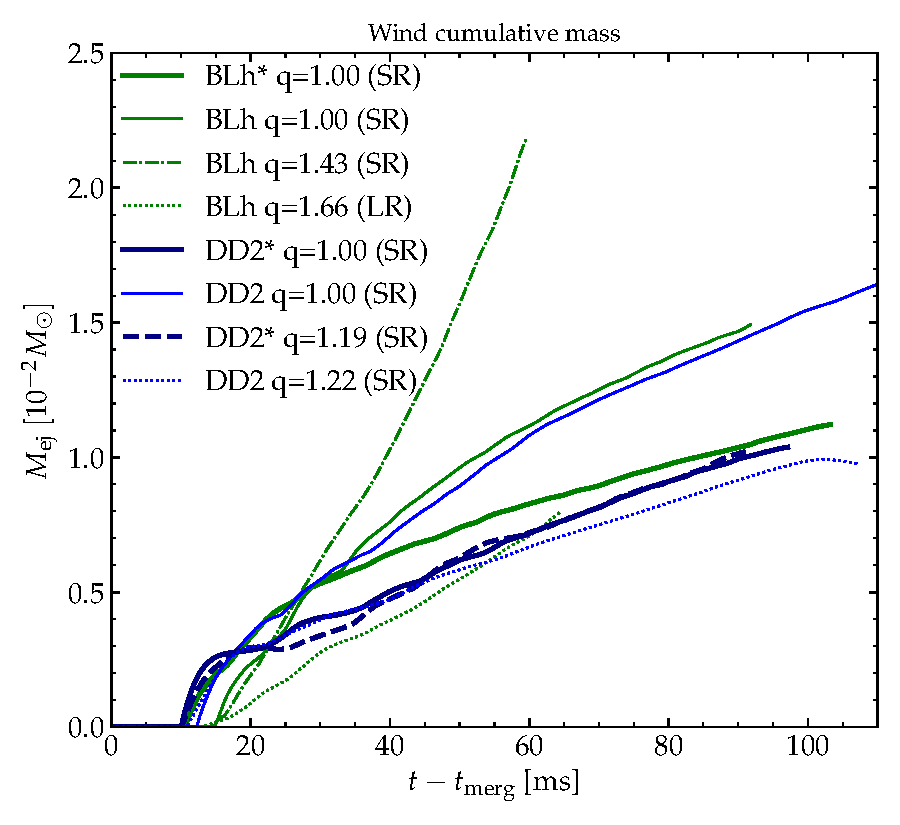
\includegraphics[width=0.50\textwidth]{ejecta_postdyn/wind_mass_flux.pdf}
    %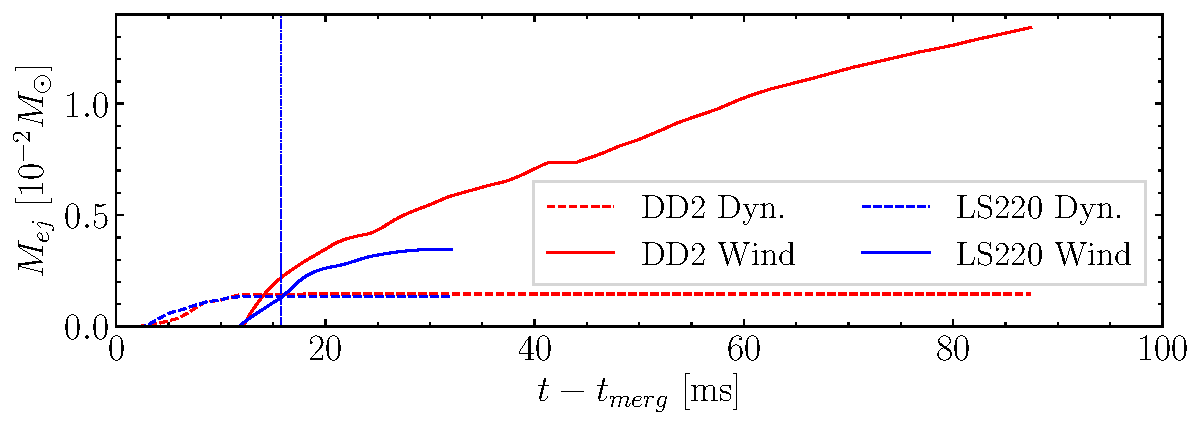
\includegraphics[width=0.55\textwidth]{ejecta_postdyn/ejecta_profiles_dd2_ls220_long.pdf}
    \caption{
        Time evolution of the cumulative \ac{SWW} mass for a set of 
        simulations with long-lived remnants. 
        Here $t_0$ indicates the moment of merger. The wind 
        calculation starts when \ac{DE} saturates ${\gtrsim}10\,$ms \pmerg{}.
%        \emph{Left panel}:
%        Cumulative mass of the \swind{} from long-lived
%        remnants. The wind persists on timescales of $\mathcal{O}(100)\,$ms with
%        mass fluxes ${\sim}0.33-1.23\,\Msun/s$.
%        Adapted from \citet{Nedora:2020pak}.
%        \emph{Right panel}:
%        Evolution of unbound mass for dynamical ejecta
%        (dashed lines)
%        and \swind{}
%        (solid lines). $t=0$ marks the moment of merger, the vertical
%        line marks the collapse time of the model with LS220 \ac{EOS}.
        Adapted from \citet{Nedora:2019jhl}.
    }
    \label{fig:mej:bern}
\end{figure}

%\begin{figure}[t]
%    \centering 
%    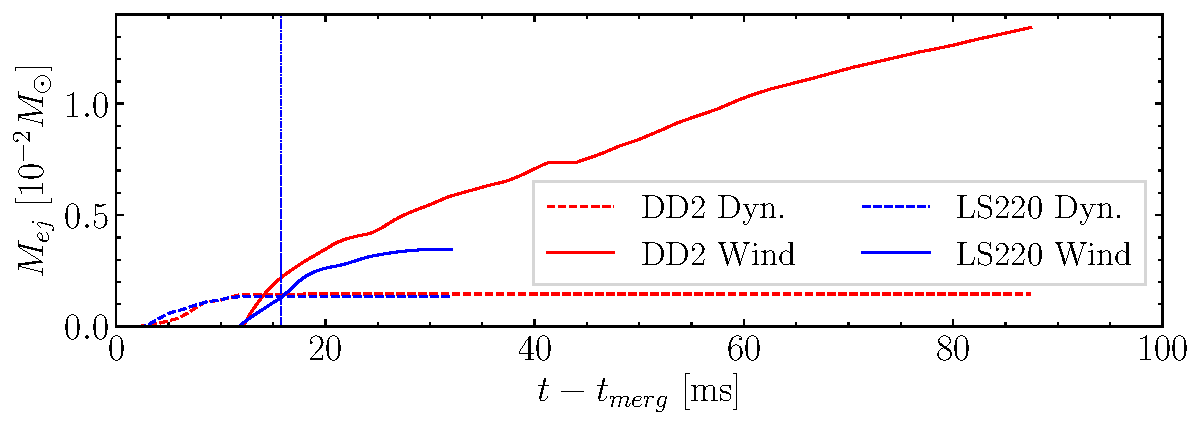
\includegraphics[width=0.70\textwidth]{ejecta_postdyn/ejecta_profiles_dd2_ls220_long.pdf}
%    \caption{Evolution of unbound mass for dynamical ejecta
%        (dashed lines)
%        and \swind{}
%        (solid lines). $t=0$ marks the moment of merger, the vertical
%        line marks the collapse time of the model with LS220 \ac{EOS}.
%        Adapted from \cite{Nedora:2019jhl}.
%    }
%    \label{fig:mej:bern_short_long}
%\end{figure}

\begin{figure*}[t]
    \centering 
    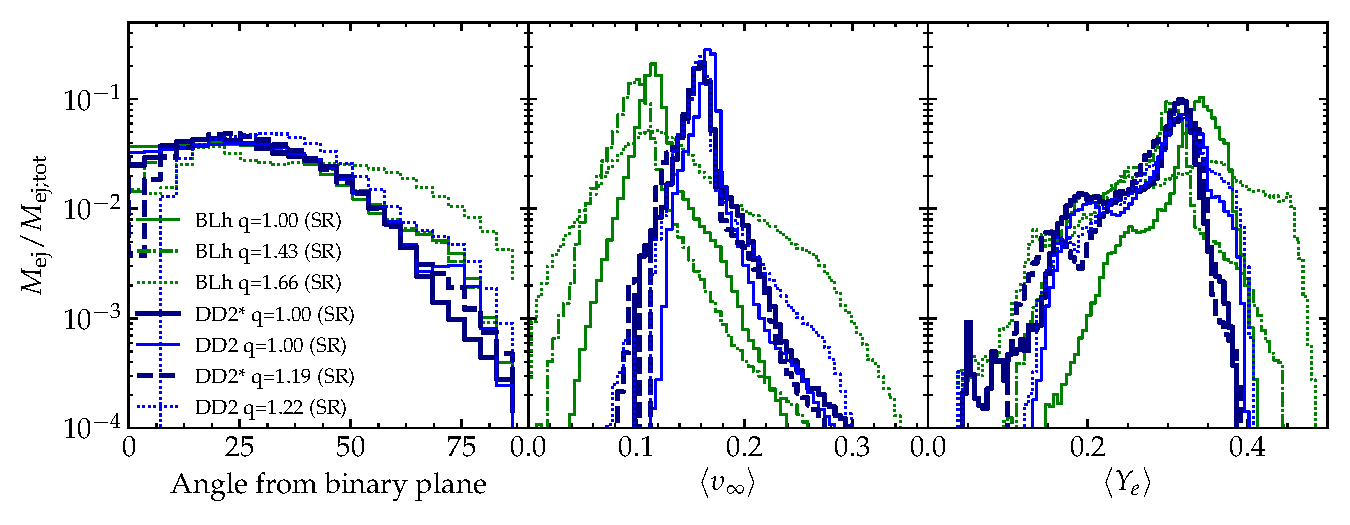
\includegraphics[width=0.99\textwidth]{ejecta_postdyn/wind_hists_shared.pdf}
    \caption{
        Properties of the \ac{SWW} from the set of simulations with long-lived 
        remnants. From left tow right, the angular, velocity and electron fraction 
        distributions are shown in a from of mass-histograms. 
%        Mass-averaged histograms of the \swind{} for a selected
%        subset of long-lived remnant. From left to right: ejecta angular
%        distribution, ejecta terminal velocity and electron
%        fraction. Remnants from more asymmetric binaries produce winds
%        with broader angular distribution.
%        The \swind{} from the DD2 EOS remnants has larger velocities
%        then the winds from the softer BLh EOS. The electron fraction
%        peaks at ${\sim}0.3$ and it is distributed from $0.1$ to $0.4$.
        (Adapted from \citet{Nedora:2020pak}).
    }
    \label{fig:ejecta:bern:hist}
\end{figure*}

%\begin{figure}[t]
%    \centering
%    %% 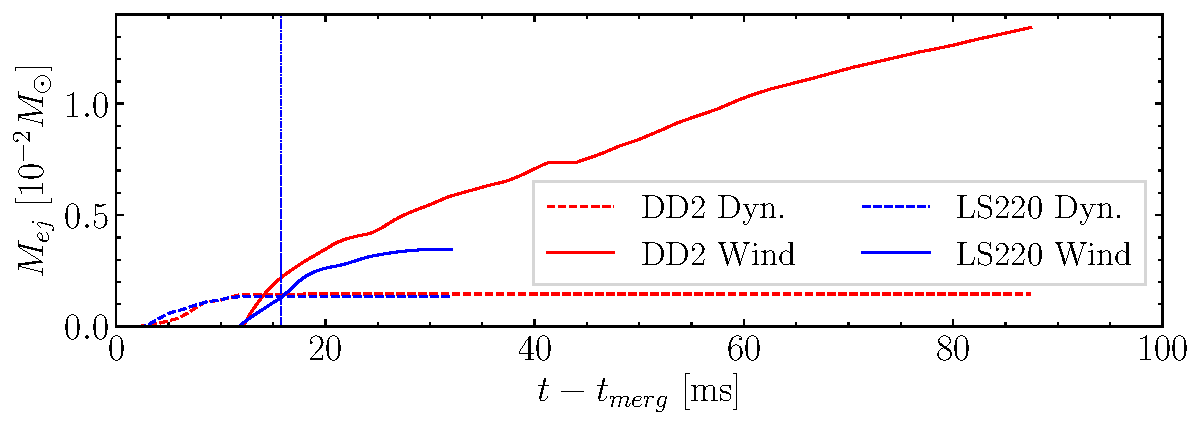
\includegraphics[width=0.49\textwidth]{ejecta_postdyn/ejecta_profiles_dd2_ls220_long.pdf}
%    %% 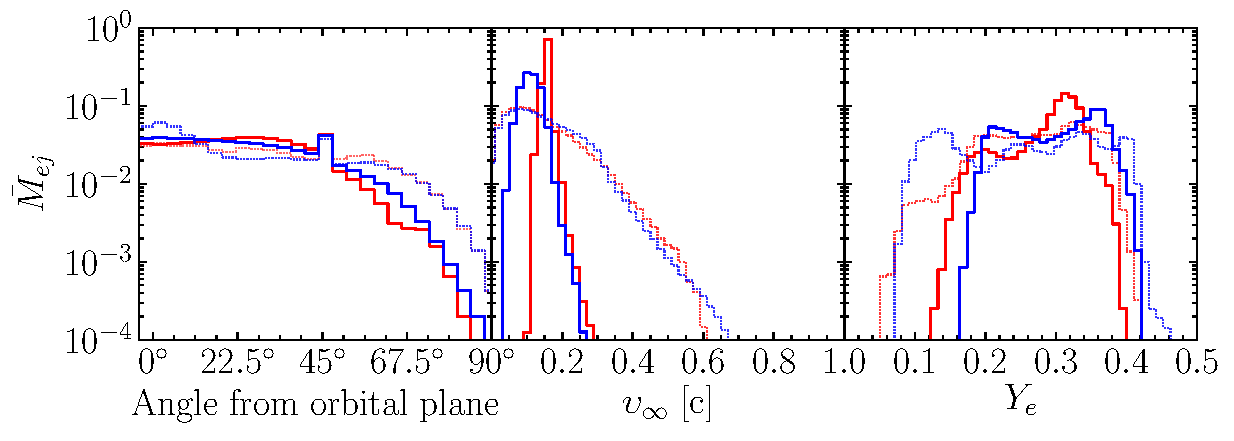
\includegraphics[width=0.49\textwidth]{ejecta_postdyn/hist_1D_dd2_ls220_long.pdf}
%    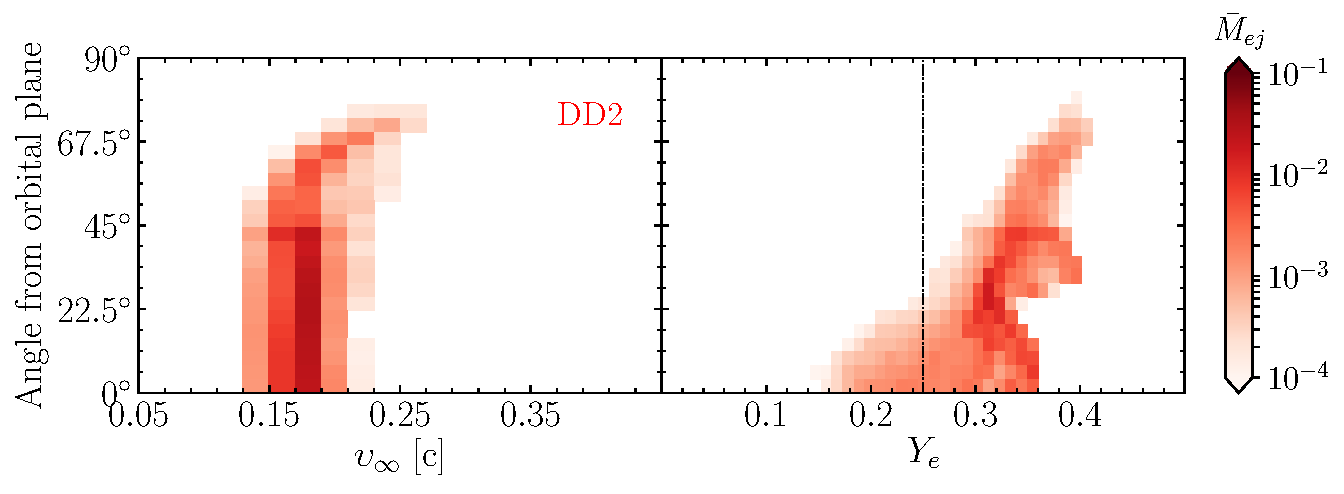
\includegraphics[width=0.75\textwidth]{ejecta_postdyn/corr_dd2.pdf}
%    \caption{Properties of the \ac{SWW} and dynamical ejecta
%        computed form the simulations with turbulent viscosity.
%        %
%        Top: evolution of unbound mass for dynamical ejecta
%        (dashed lines)
%        and \ac{SWW}
%        (solid lines). $t=0$ marks the moment of merger, the vertical
%        line marks the collapse time of the LS220 BNS.
%        %
%        Middle: mass histograms for the angular (left), velocity (center) and electron
%        fraction (right) distributions.
%        Bottom: angular distribution and composition of the \ac{SWW}
%        for DD2.
%        %
%        Note the $\bar{M}_{ej}$ in the middle and bottom panels is normalized to one.
%        (Adapted from \citet{Nedora:2019jhl})
%    }
%    \label{fig:ej_properties}
%    
%\end{figure}

%% --------------------------------
%% TAB WIND SUMMARY
\begin{sidewaystable}
%\begin{table*}[t]
  \centering
  \captionsetup{width=1.0\linewidth}
  \caption{%
    Summary table of the \swind{} properties of long-lived remnants. The columns contain
    the following information, starting from the left. Equation of
    state, mass-ratio, available resolutions,
    inclusion of subgrid turbulence, time of the
    simulation end, mass of the
    \swind{}, mass-loss rate via \swind, mass-averaged electron fracton, terminal
    velocity and, finally, RMS angle for \swind{}. For these four
    quantities we give the mean value among the resolutions and
    one-sigma deviations. For binaries for which only one
    resolution is present, the error is assumed to be $20\%$ of the value.
    (Adapted from \cite{Nedora:2020pak}).
    }
  \label{tab:spiralwavewind}
  \begin{tabular}{c c c c c c c c c c}
    \hline\hline
    EOS & $q$ & Resolution & GRLES & $t_{\text{end}}$ & $\amw$ & $\amw/\Delta t$ & $\ayw$ & $\avw$ & $\langle \theta_{\text{ej}}^{\text{w}} \rangle$ \\
    &   &   &   & [ms] & $[10^{-2} M_{\odot}]$ & $[M_{\odot}/s]$ &   & $[c]$ &   \\ 
    \hline
    \hline
    BLh & 1.00 & \texttt{SR HR LR} & \cmark & $43.3$ $91.8$ $23.1$ & $0.39^{+0.07} _{-0.07} $ & $0.70^{+0.32} _{-0.32} $ & $0.31^{+0.01} _{-0.01} $ & $0.12^{+0.01} _{-0.01} $ & $27.06^{+2.61} _{-2.61} $ \\
    BLh & 1.00 & \texttt{SR} & \xmark & $ $ $103.2$ $ $ & $1.12^{+0.57} _{-0.57} $ & $1.07^{+0.21} _{-0.21} $ & $0.34^{+0.01} _{-0.01} $ & $0.12^{+0.02} _{-0.02} $ & $15.72^{+2.00} _{-2.00} $ \\
    \hline
    BLh & 1.18 & \texttt{LR} & \cmark & $69.4$ $ $ $ $ & $1.28^{+0.64} _{-0.64} $ & $1.23^{+0.25} _{-0.25} $ & $0.33^{+0.01} _{-0.01} $ & $0.11^{+0.02} _{-0.02} $ & $14.98^{+2.00} _{-2.00} $ \\
    \hline
    BLh & 1.43 & \texttt{LR SR} & \cmark & $35.1$ $59.6$ $ $ & $0.75^{+0.18} _{-0.18} $ & $1.06^{+0.67} _{-0.67} $ & $0.27^{+0.01} _{-0.01} $ & $0.09^{+0.01} _{-0.01} $ & $19.43^{+2.22} _{-2.22} $ \\
    \hline
    BLh & 1.54 & \texttt{LR} & \cmark & $45.8$ $ $ $ $ & $0.63^{+0.32} _{-0.32} $ & $0.44^{+0.09} _{-0.09} $ & $0.32^{+0.01} _{-0.01} $ & $0.10^{+0.02} _{-0.02} $ & $21.46^{+2.00} _{-2.00} $ \\
    \hline
    BLh & 1.66 & \texttt{LR SR} & \cmark & $64.6$ $20.1$ $ $ & $0.12^{+0.09} _{-0.09} $ & $0.37^{+0.34} _{-0.34} $ & $0.33^{+0.05} _{-0.05} $ & $0.13^{+0.01} _{-0.01} $ & $52.08^{+20.89} _{-20.89} $ \\
    \hline
    \hline
    DD2 & 1.00 & \texttt{LR SR HR} & \cmark & $123.0$ $113.0$ $74.4$ & $1.25^{+0.14} _{-0.14} $ & $1.30^{+0.19} _{-0.19} $ & $0.30^{+0.01} _{-0.01} $ & $0.17^{+0.00} _{-0.00} $ & $14.88^{+0.87} _{-0.87} $ \\
    \hline
    DD2 & 1.20 & \texttt{LR SR HR} & \xmark & $37.3$ $91.0$ $55.2$ & $0.48^{+0.09} _{-0.09} $ & $0.74^{+0.24} _{-0.24} $ & $0.26^{+0.01} _{-0.01} $ & $0.15^{+0.00} _{-0.00} $ & $24.54^{+2.23} _{-2.23} $ \\
    \hline
    DD2 & 1.43 & \texttt{LR SR} & \cmark & $37.7$ $62.0$ $ $ & $0.60^{+0.02} _{-0.02} $ & $0.51^{+0.06} _{-0.06} $ & $0.23^{+0.12} _{-0.12} $ & $0.16^{+0.00} _{-0.00} $ & $21.74^{+0.03} _{-0.03} $ \\
    \hline
    \hline
    SFHo & 1.43 & \texttt{SR} & \cmark & $ $ $46.5$ $ $ & $0.58^{+0.30} _{-0.30} $ & $0.43^{+0.09} _{-0.09} $ & $0.31^{+0.01} _{-0.01} $ & $0.17^{+0.02} _{-0.02} $ & $22.67^{+2.00} _{-2.00} $ \\
    \hline
    \hline
    SLy4 & 1.43 & \texttt{SR} & \cmark & $ $ $40.3$ $ $ & $0.53^{+0.27} _{-0.27} $ & $0.38^{+0.08} _{-0.08} $ & $0.29^{+0.01} _{-0.01} $ & $0.18^{+0.02} _{-0.02} $ & $23.52^{+2.00} _{-2.00} $ \\
    \hline\hline
\end{tabular}
%\end{table*}
\end{sidewaystable}

%% --------------------------------

As was discussed above, the interaction between the \ac{NS} remnant and the disk 
generates density waves that propagate outwards through the disk and induce massive outflows, 
the \ac{SWW} (see Sec.~\ref{sec:bns_sims:remdisk}).
%
We track the \ac{SWW} as the matter unbound according to the Bernoulli criterion 
%$hu_t < -1$, with $h$ being the fluid enthalpy and $u_{\alpha}$ its four-velocity,
(see Sec.~\ref{sec:bns_sims:method:ejecta}). 
%
The ejecta properties are extracted at $R=294\,$km, after the \ac{DE} mass 
flux has saturated (\eg, ${\gtrsim}10\,$ms \pmerg{}).
%
%The ejecta calculation is turned on when
%the \ac{DE} mass flux stops, which on average corresponds to ${\sim10}$~ms \pmerg{} 
%

%\subsubsection{Spiral wave wind and the remnant lifetime}

%

%We start by considering two representative models, 
%DD2 $q=1.00$ (\texttt{SR}) and LS220 $q=1.00$ (\texttt{SR}), that produce 
%long- and short-loved remnants respectively, 
%We find that if the remnant is long-lived, total \ac{SWW} mass exceeds that of 
%the \ac{DE}. %  as shown also in Fig.~\ref{fig:mej:bern}.
%
%First we consider two representative models that produce long- and short-lived
%remnants. Simulations have $q=1.00$ and DD2 and LS220 \acp{EOS} respectively.
%We find that if the remnant is long-lived, total \ac{SWW} mass exceeds that of the \ac{DE},
%as shown also in Fig.~\ref{fig:mej:bern_short_long}.
%
%This is a simple consequence of the fact the \ac{SWW} mass flux continues for as long as 
%remnant survives.
%
%The inclusion of turbulent viscosity alters all the ejecta masses with an
%additional component \citep{Radice:2018ghv} and, we observe that, it enhances the 
%\ac{SWW} mass by ${\sim}25$\% in the case of DD2 $q=1.00$ model,
%exceeding the finite resolution effects. 
%%\red{Letter stuff. Not sure if true}
%%ac factor that exceeds the resolution effects.
%%
%The latter are ${\sim}15\%$ and ${\sim}8\%$ for the \ac{SWW} mass when the 
%resolution increases from \texttt{SR} to \texttt{HR}.
%The resolution effects on other wind properties, \eg, velocity and $Y_e$, 
%is found to be within $4\%$.
%
%Specifically, we find that the \ac{SWW} mass increases by ${\sim}+15\%$ and
% ${\sim}+8\%$, 
%when the resoltuion increases from LR to SR and from SR to HR respectively.
%Hence, finite grid effects tend to increase mass. A similar analysis on the average 
%electron fraction and velocity indicate variations below $4\%$.
% --- Repetition below
%The angular distribution of the \ac{SWW} resembles that of the \ac{DE} and is 
%largely equatorial, as shown in Fig.~\ref{fig:ej_properties}. 
%%
%The velocity distribution,
%however, is rather different with a narrow peak around $0.1-0.2\,$c, depending on the 
%stiffness of the \ac{EOS}. Notably, properties of the \ac{SWW} are sensitive to the 
%lifetime of the remnant, as at early times they are modified by the trace presence of the 
%\ac{DE} and not-yet-relaxed \pmerg{} environment.
%%
%The electron fraction of the \ac{SWW} also shows a narrow distribution with a peak 
%at ${\geq}0.25$, which is considerably higher than that of the \ac{DE}. 
%Notably, the electron fraction is lower if the remnant is short-lived as it 
%disks around NS remnants are less compact, colder, and optically thicker than those 
%around black holes~\citep{Perego:2019adq}, the outer layers of the DD2 disk have a
%lower $Y_e$ than the LS220 disk and so does the \ac{SWW} coming from those layers.

%\gray{
%    %% From Letter
%    The \ac{SWW} has an angular distribution of mass similar to the
%    dynamical ejecta with material mostly confined to the orbital plane,
%    as shown by the histograms in Fig.~\ref{fig:ej_properties}.
%    On the contrary, the velocity profiles show a drastic difference
%    between the two ejecta components. While the dynamical ejecta has a
%    broad velocity distribution \citep{Hotokezaka:2012ze,Bauswein:2013yna,Radice:2018pdn}, the 
%    \ac{SWW} velocity is narrowly distributed around  
%    $0.2$c in the case of a long-lived remnant (DD2).
%    The \ac{SWW} from the short-lived
%    remnant (LS220) has a broader velocity distribution extending down to
%    $0.1$c.
%    This is due to the spiral-wave shutting down and the disk
%    transition to a more steady accretion. As a consequence, the \ac{SWW}
%    ceases but ejecta continue as a slower disc wind driven
%    by nuclear recombination solely.
%    The electron fraction of the \ac{SWW} has a
%    narrower distribution than the dynamical ejecta in both
%    cases. But because disks around NS remnants are less compact, 
%    colder, and optically thicker than those around black
%    holes~\citep{Perego:2019adq}, the outer layers of the DD2 disk have a 
%    lower $Y_e$ than the LS220 disk and so does the \ac{SWW} coming from
%    those layers.
%    While the \ac{SWW} is generic in its hydrodynamics origin, the
%    quantification of its properties relies on the accurate microphysics and
%    neutrino treatment in our simulations.
%}

% \subsubsection{Spiral wave wind for all models}

We report the overall properties of the \ac{SWW} for all models with 
long-lived \ac{NS} remnants that were also evolved for a sufficiently long time 
in the Tab.~\ref{tab:spiralwavewind}. 
%
The time evolution of the total mass of the \ac{SWW} is shown in  Fig.~\ref{fig:mej:bern}.
We observe that in all simulations \ac{SWW} persists till the time these simulations 
were terminated at without saturation.
This is the manifestation of the mechanism, driving the outflow: the 
angular momentum and mass transport induced by the dynamical instabilities in the 
remnant, the $m=1,2$ modes. And, as the $m=1$ modes are not efficiently damped \citep{Paschalidis:2015mla,Radice:2016gym,Lehner:2016wjg,East:2016zvv},
the \ac{SWW} could theoretically continue until the system collapses to a \ac{BH} 
or reaches an equilibrium. % (Sec.~\ref{sec:bns_dynsmics_overview}).
%
The strongest \ac{SWW} is found in binaries with $q>1$, such as 
BLh $q=1.43$ (\texttt{SR}) model. 
With the mass-loss rate ${\sim}0.5\, \Msun/{\text{s}}$, these models can eject 
${\sim}0.02\,\Msun$ within ${\sim}50\,$ms of the \pmerg{} evolution.
%
Meanwhile, models with softer \acp{EOS} reach similarly high mass flux 
at lower \mr{}s. For instance, the \ac{SWW} mass flux of BLh* $q=1.66$ model 
is achieved by the LS220* $q=1.22$ model. 
A possible explanation for this is that the models with softer \acp{EOS} have stronger 
$m=1$ modes in the remnant (see Sec.~\ref{sec:bns_sims:remdisk}).

The inclusion of turbulent viscosity alters all the ejecta masses with an
additional component \citep{Radice:2018ghv} and, we observe that, it enhances the 
\ac{SWW} mass by ${\sim}25$\% in the case of DD2 $q=1.00$ model,
exceeding the finite resolution effects. 
%\red{Letter stuff. Not sure if true}
%ac factor that exceeds the resolution effects.
%
The latter are ${\sim}15\%$ and ${\sim}8\%$ for the \ac{SWW} mass when the 
resolution increases from \texttt{SR} to \texttt{HR}.
The resolution effects on other wind properties, \eg, velocity and $Y_e$, 
is found to be within $4\%$.

When a \ac{NS} remnant collapses to a \ac{BH} and the mechanism that injects angular 
momentum into the disk shuts down, the \ac{SWW} mass flux subsides.
% (right panel of  Fig.~\ref{fig:mej:bern}). 
Thus, the total ejected mass via \ac{SWW} is directly related to the lifetime of the 
\ac{NS} remnant, in addition to the binary parameters, \ac{EOS} and \mr{}.
%
The \ac{SWW} mass flux depends on the disk configuration as more extended disks 
have outer layers that are less gravitationally bound. In turn, the disk 
configuration is dependent on the thermal effects. Higher temperature leads to 
stronger thermal pressure that increases the disk size. 
However, the dependency of the \ac{SWW} mass flux on the stiffness of the \ac{EOS} 
appears to be stronger, as stiffer \acp{EOS} lead to more massive disks, 
as discussed in Sec.~\ref{sec:bns_sims:remdisk}.   % contradiction with [1]
%(Fig.~\ref{fig:disk_mass_evo}). 
More simulations with longer \pmerg{} evolution are needed 
to make a quantitative assessment. 
%Overall the \swind{} from the long-lived remnant has a mass flux $\geq 0.4\, \Msun/{\text{s}}$.

%TODO cd ~; cp ~/Tullio/prj_gw170817/BLh_M13641364_M0_LK_SR/{slice_xz_ye_hu_1.pdf,slice_xz_abs_energy_hu_3.pdf,slice_xy_ye_hu_1.pdf,slice_xy_abs_energy_hu_3.pdf} ~/GIT/GitHub/phd_thesis/v4/Figures/slices/
\begin{figure*}[t]
    \centering 
    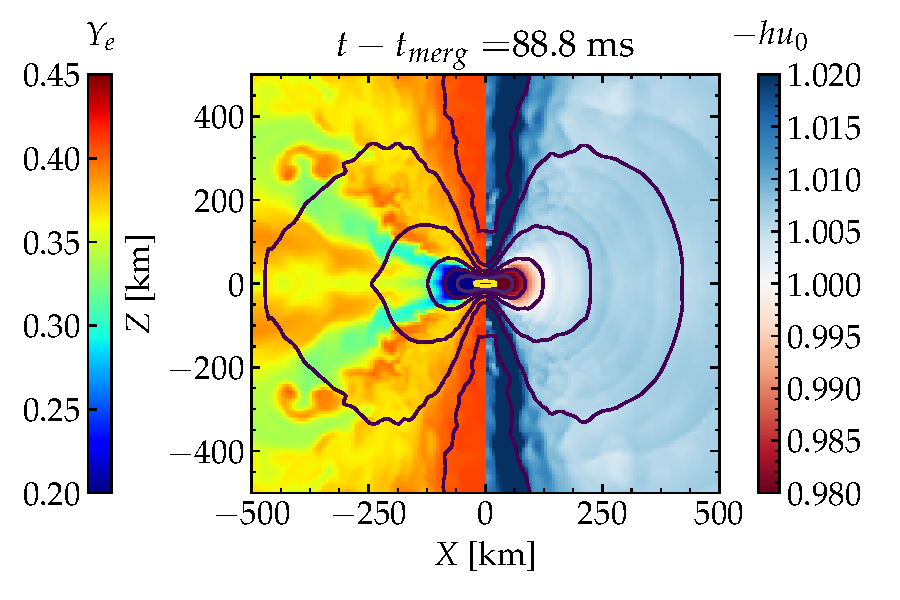
\includegraphics[width=0.49\textwidth]{slices/slice_xz_ye_hu_1.pdf}
    \hspace{-5mm}
    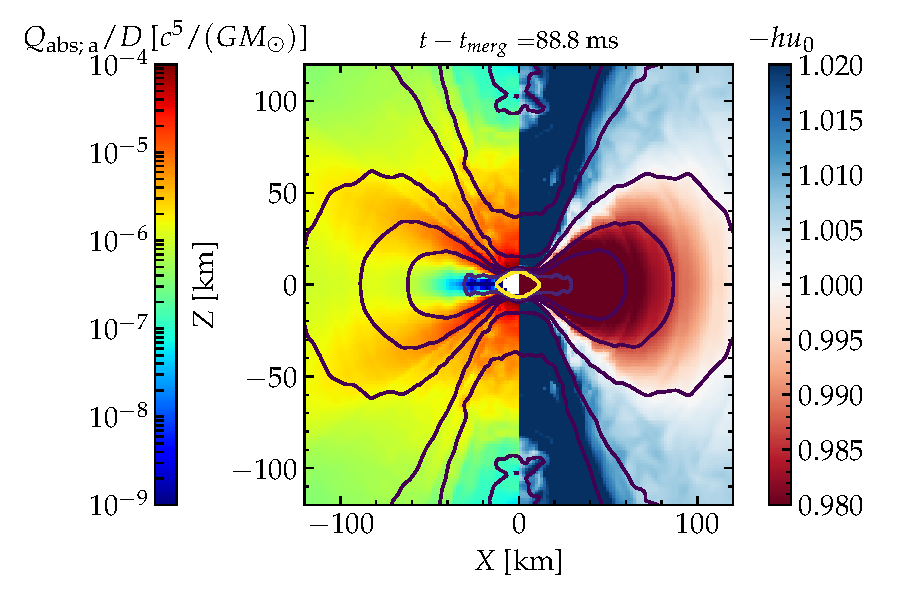
\includegraphics[width=0.49\textwidth]{slices/slice_xz_abs_energy_hu_3.pdf}
    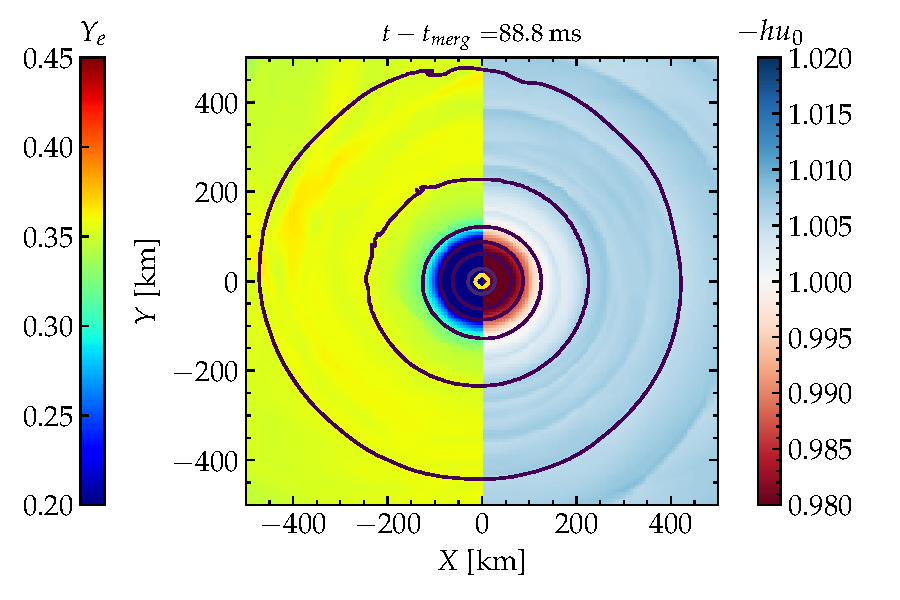
\includegraphics[width=0.49\textwidth]{slices/slice_xy_ye_hu_1.pdf}
    \hspace{-5mm}
    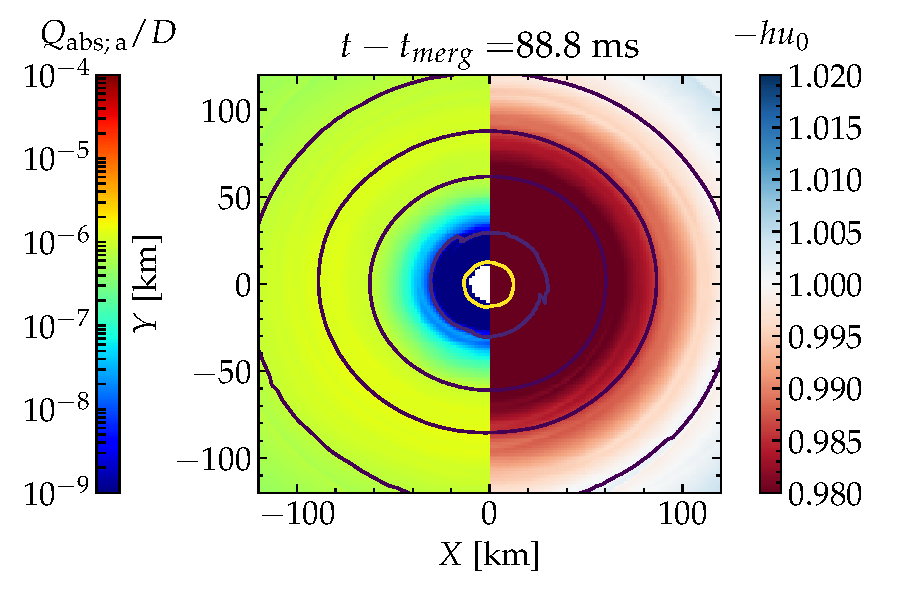
\includegraphics[width=0.49\textwidth]{slices/slice_xy_abs_energy_hu_3.pdf}
    \caption{
        Snapshots of the BLh $q=1.00$ model taken $88\,$ms \pmerg{}, 
        showing the distribution of electron fraction, $Y_e$, 
        Bernoulli parameter, $-hu_t$, and electron anti-neutron 
        absorption energy rate, $Q_{\text{abs};\:\bar{\nu}_e}$ 
        normalized to the fluid density $D$ in units of $c^{5}/(G M_{\odot})$. 
        \textit{Top row of panels} displays these properties in $(x,z)$ plane, 
        while the \textit{bottom row} shows $(x,y)$ slices. 
%        Snapshots of the BLh $q=1.00$ model taken $88\,$ms \pmerg{}, 
%        displaying the distribution of the electron fraction, $Y_e$, 
%        (\textit{left side of each panel of the right column of panels}), 
%        Bernoulli parameter, $-hu_t$,
%        Snapshot of the $(x,z)$ and $(x,y)$ slices of the BLh $q=1$ model at 
%        ${\sim}89\,$ms after merger. Left panels: electron fraction and
%        $-hu_0$. High $Y_e$ values indicate neutrino
%        postprocessing and irradiation. The $-hu_0>1$ indicates the
%        material that gains enough energy to become unbound at
%        infinity. 
%        %
%        Right: $-hu_0$ and the absorption energy rate $Q_{\text{abs};\:\bar{\nu}_e}$ 
%        of electron antineutrinos normalized to the fluid density $D$.
        %
        (Adapted from \citet{Nedora:2020pak}).
    }
    %
    \label{fig:slice:heating_hu}
\end{figure*}

We find that contrary to the mass flux, other properties of the \ac{SWW} 
depend only weakly on the binary parameters,
\mr{} and \ac{EOS}. Mass-histograms of the wind angular distribution, velocity and 
electron fraction are displayed in Fig.~\ref{fig:ejecta:bern:hist} for representative models. 
The angular distribution of the \ac{SWW} is similar to that of the \ac{DE}. The ejecta 
has a broad distribution around the binary plane.
The \ac{SWW} has high average electron fraction. Its overall broad distribution,  
$0.1\lesssim \ayw\lesssim0.4$, peaks at ${\simeq}0.35$.
The low electron fraction material originates primarily at early times, when the 
material did not have enough time to be processed by neutrinos and before the 
outflow reaches quasi-steady state.
The \ac{SWW} average velocity is higher for stiffer \acp{EOS}, with the peak 
of the distribution laying between ${\sim}0.1\,$c and ${\sim}0.2\,$c.
However, more simulations of the \ac{NS} remnants long-term evolution are 
required to confirm and quantitatively investigate these trends.
%However, if it is indeed a generic feature, then it might imply 
%an \ac{EOS} dependent distinct feature in the electromagnetic counterpart. 
%In particular, the observation of a fast blue kN given by the \swind{}
%should be associated to a stiff \ac{EOS}.

%% It is however expected, that as the system becomes more stationary and larger part 
%% of the disk accrets on the \ac{MNS} the outflow should subside. 


\subsection{Neutrino-driven wind} \label{sec:bns_sims:nwind}



%In this section we focus on the high electron fraction, polar component of the 
%\acp{SWW}. 

In Sec.~\ref{sec:intro:ejecta} we discussed that in the presence of strong 
neutrino fluxes, baryonic winds may emerge being driven by these neutrino fluxes.  
Since the strongest source of neutrinos is \ac{NS} remnant, such an outflow,
\nwind, is expected to be polar and characterized by elevated electron fraction 
\citep[\eg][]{Perego:2014fma}. 
%
Having neutrino absorption included in our simulation setup (See 
Sec.~\ref{sec:nr_methods:neut}), we assess whether there is \nwind{} in our 
simulations. Naturally, we expect it to be a part 
of the \ac{SWW}, polar and with high $Y_e$. 
%
For this analysis, for the sake of brevity, we focus on one 
simulation, BLh $q=1.00$ (\texttt{SR}). 


%
In the left column of plots in Fig.~\ref{fig:slice:heating_hu} we compare 
the the Bernoulli parameter, $-hu_t$, 
%(see Sec.\ref{sec:bns_sims:method:ejecta}),
and the fluid electron fraction. 
%
In the right column of plots in Fig.~\ref{fig:slice:heating_hu} we compare 
the the Bernoulli parameter with the heating energy rate due to electron anti-neutrino absorption, 
$Q_{\text{abs};\:\bar{\nu}_e}$, computed by the M0 scheme 
(see Sec.~\ref{sec:nr_methods:neut}) and 
normalized with fluid's conserved rest-mass density.
% and divided by $D=W\rho\sqrt{\gamma}$ 
%(fluid's conserved rest-mass density).
We observe that the electron fraction in the polar region  
($\theta>60^{\circ}$, where $\theta$ is the angle from the binary plane) 
reaches $Y_e\sim0.35$ due to the absorption of 
electron-type anti-neutrinos.
The strongest neutrino heating occurs in the vicinity of the remnant at densities 
$\rho\sim10^{11}$~\gcm{} that roughly correspond
to the location of the neutrinosphere \citep{Endrizzi:2019trv}, 
the region where neutrinos decouple from matter.
%
% to the region where neutrinos decouple,
%the so-called neutrinosphere \citep{Endrizzi:2019trv}.
%
%In Fig.~\ref{fig:slice:heating_hu} we also compare the Bernoulli parameter, 
%$-hu_t$ (see Sec.\ref{sec:bns_sims:method:ejecta}), 
%that is always plotted 
%on the right half of a panel, with the electron fraction (left 
%column of plots and heating energy rate due to electron anti-neutrino absorption 
%$Q_{\text{abs};\:\bar{\nu}_e}$ divided by with $D=W\rho\sqrt{\gamma}$ 
%(fluid's conserved rest-mass density).
%The observed correlation between the $E_\nu/D$ \red{???} and $-h u_t$ further suggests, 
%that the outflow around the polar axis is driven by the neutrino absorption. 
Additionally, we found that if the neutrino absorption is not included into the 
simulation, \eg, using leakage scheme only, the \nwind{} is significantly suppressed.  %\red{bullshit}
%
%The collimated polar outflow can be further boosted and stabilized by the presence of the 
%strong magnetic fields \citep{Bucciantini:2011kx,Ciolfi:2020hgg,Mosta:2020hlh}.

Notably, there is no clear distinction between the \nwind{} and \ac{SWW}, especially 
at intermediate latitudes ($\theta \sim 45^{\circ}$) where both mechanisms and 
types of ejecta are present.
%, and both, neutrino absorption and dyanmical effects 
%driving the \ac{SWW} are contributing. 
%
In order to compute the mass flux of the \nwind{} we impose an additional criteria.
%to the Bernoulli, criteria.
We consider two physically motivated options, the geometrical, flagging the part of 
the \ac{SWW} as \nwind{} if it is polar, \ie, $\theta>60^{\circ}$, and the 
composition criterion, \ie, if $Y_e > 0.35$.
%
We find that the \nwind{} is not a steady state outflow, contrary to the 
bulk of the \ac{SWW}. After the initial strong rise, the mass flux rapidly 
decays in time, and for most models stops before the simulation is terminated. 
This behaviour is independent of the criterion we use. We attribute this to the 
rise of the baryon loading above the remnant as the material gets lifted 
by the thermal pressure from the disk.
The total mass of the \nwind{} is ${\sim}10^{-3}-10^{-4}M_{\odot}$. Its 
properties resemble those reported in \eg, 
\citet{Dessart:2008zd,Perego:2014fma,Fujibayashi:2020dvr}.
Notably, in some of the works, the \nwind{} was found to require longer 
timescales to develop. %, achieving the quasi-steady state. 
This can be attributed to the strict criteria to isolate the \nwind{} and by 
the absence of the \ac{SWW} in other works. 
Additionally, our simulations might not be sufficiently long to achieve the 
conditions sufficient for the development of the quasi-steady state \nwind{}.
%% Additionally, as our models are at most $\sim100$~ms long, the conditions required for the steady 
%% state \nwind{} might not been achieved.



%% =======================================================
%%
%%                   Disc structure
%%
%% =======================================================




%\red{Paragraph on the secular ejecta has been moved to 
%    GW170817 application}

%% =======================================================
%%
%%                   Conclusion
%%
%% =======================================================




%% ========================================================================================

%\section{Statistics of the \ac{DE} parameters and disk mass}
%
%\red{CONTENT OF THE FIT PAPER}
%
%
%\section{Application to \GW{}}
%
%
%\begin{figure*}[t]
%    \centering 
%    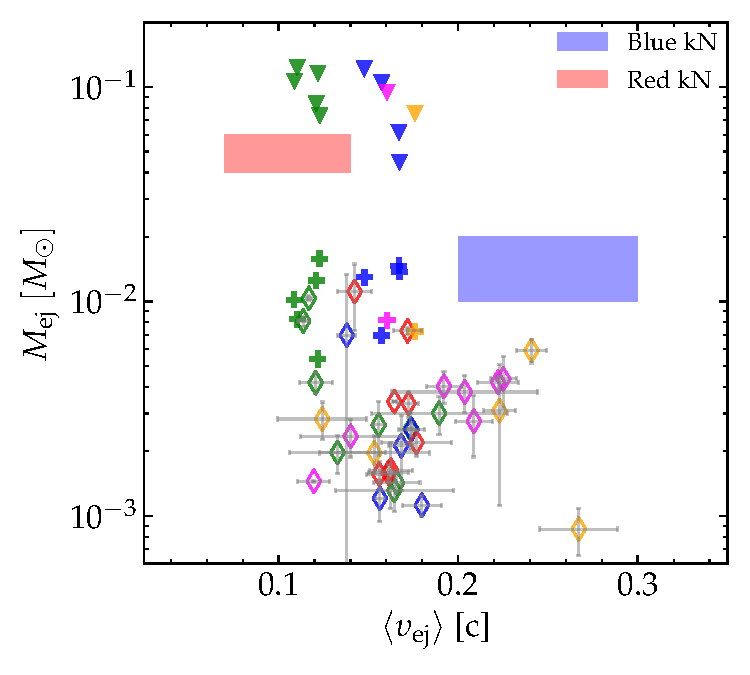
\includegraphics[width=0.48\textwidth]{ejecta_dyn/summary/ej_mej_vej_our2.pdf}
%    \includegraphics[width=0.48\textwidth]{ejecta_dyn/summary/ej_mej_yeej_our2.pdf}
%    \caption{
%        Summary of the ejecta properties of our models.
%        %
%        Diamonds mark the dynamical ejecta, crosses include the
%        contribution of the \swind{} for the long-lived models, 
%        triangles are an estimate of the total ejecta mass on a secular
%        timescale, assuming $40\%$ of the disk mass is unbounded on
%        secular timescales.         
%        The ejecta mass is shown is terms of the mass-averaged velocity
%        (left) and of the averaged electron fraction (right).
%        %
%        The filled blue and red patches are the expected values of
%        ejecta mass and velocity for blue and red components of
%        AT2017gfo compiled by \cite{Siegel:2019mlp}, based on
%        \cite{Villar:2017wcc}. 
%        Adopted from \citet{Nedora:2020pak}.
%    }
%    %
%    \label{fig:ejecta:dyn:ds_sww}
%\end{figure*}
%
%
%%% from main paper, referencing the fitpaper Poly22 fits and SWW + DE
%\red{THis can be augmented with Radio afterglow}
%
%%% === FROM DYNAMICAL EJECTA SECTION of MAIN PAPER
%Here we discuss the application of our results to \GW{}.
%
%
%\subsection{Dynamical Ejecta}
%
%
%%% ---
%First, we asses the ejecta parameters that our fitting models, 
%obtained in section \ref{sec:ejecta_disk_statisitcs} would provide for the \GW{}.
%%% --- 
%Considering the $90\%$ credible intervals estimated for $q$ and $\tilde{\Lambda}$ 
%from LIGO-Virgo GW analysis
%\citep{TheLIGOScientific:2017qsa,Abbott:2018wiz,De:2018uhw,Abbott:2018exr},
%i.e.~$\tilde{\Lambda}=300_{-190}^{+500}$ and $q\in[1., 1.37]$. 
%and using the errorbars formulas developed in \cite{Radice:2018pdn}, we find that
%$\amd \in [0.72, 7.52] \times 10^{-3}\: M_{\odot}$
%and
%$\avd \in [0.16, 0.39]$c 
%and 
%$\ayd \in [0.11, 0.23]$.
%Notably, these values do not agree with those inferred for \AT{} by the spherical, 
%two-component kilonova models \citep{Villar:2017wcc}.
%Analysis of a compiled set of kilonova fitting models provides a broad range of ejecta 
%parameters \citep{Siegel:2019mlp}:
%$M_{\text{ej}}^{\text{red}}\in(4, 6)\times10^{-2}M_{\odot}$ and
%$\upsilon_{\text{ej}}^{\text{red}}\in(0.07, 0.14)$ for the red component, while
%$M_{\text{ej}}^{\text{blue}}\in[1, 2]\times10^{-2}M_{\odot}$ and 
%$\upsilon_{\text{ej}}^{\text{blue}}\in[0.2, 0.3]$ for the blue component.
%%% ---
%With respect to our results for \ac{DE}, however, 
%none of the kilonova components can be well explained.
%%% ---
%In Fig.~\ref{fig:ejecta:dyn:ds_sww} we show the ejecta properties from
%all our models (diamonds) and the parameters inferred from the
%observations as red and blue boxes. 
%%% --- 
%With respect to the red component, we observe that \ac{DE} from our models 
%have too high average velocities and not nearly enough mass.
%This result suggests that an additional, low $Y_e$ ejecta component is required
%in order to explain the \AT{} red component 
%\citep{Perego:2017wtu,Kawaguchi:2018ptg,Nedora:2019jhl}.
%%% --- 
%A more thorough analysis of the \AT{} with better ejecta models and advanced
%radiation transport kilonova simulations are not part of the present work 
%and will be addressed in the future.
%
%
%\subsection{Spiral-wave wind}
%
%
%The \ac{SWW} could be a significant contributor to the \AT{}, assuming the remnant of 
%\GW{} \ac{MNS} merger survived for $\mathcal{O}(100)$~ms.
%%% ---- 
%In Fig.~\ref{fig:ejecta:dyn:ds_sww} we report the total
%(dynamical+\swind{}) ejecta mass and mass-averaged velocity for the
%simulated long-lived BNS (crosses).
%%% ---
%Notably, the total ejecta mass of three of our models, 
%BLh $q=1.18$, BLh $q=1.42$ and  DD2 is $q=1$ are in agreemnt with the epected values 
%for the blue compoent of the \AT{} 
%(obtained using the two-component fit \citep{Villar:2017wcc})
%
%\red{
%    [ LETTER STUFF COULD GO HERE ]
%    a multi-component fitting model that explicitly accounts
%    for the \swind{} can fit the early blue
%    emission from AT2017gfo \citep{Nedora:2019jhl}
%}
%
%The high electron fraction of the \ac{SWW} however would result in a lanthanides-poor
%composition of the outflow. Thus, the \ac{SWW} cannot explain the observed emission 
%for the high opacity, lanthanides-rich material.
%%% ---
%Simulations with advanced physics of a \ac{MNS} mergers on a timescales $>100$~ms are 
%required to asses the contribution from other outflow mechanisms, \red{that we will discuss below} 
%\citep{Lee:2009uc,Fernandez:2015use,Siegel:2017nub,Fujibayashi:2017puw,Fernandez:2018kax,Radice:2018xqa}.
%
%
%\subsection{Secular Ejecta}
%
%
%On the timescale of seconds, much longer than the evolution of 
%presented here simulations, the nuclear recombination can unbind 
%a fraction of the disk mass. 
%Analytical estimates and simulations with various approximations show that up tp ${\sim}40\%$ of the disk can be ejected via viscous processes with an typical velocity ${\lesssim}0.1\,$c
%\citep{Lee:2009uc,Fernandez:2015use,Wu:2016pnw,Siegel:2017nub,Fujibayashi:2017puw,Fernandez:2018kax,Radice:2018xqa,Fujibayashi:2020dvr}.
%
%Adapting the fix fraction of the $40\%$ of the disk mass, we estimate 
%that about  ${\sim}0.05\, M_{\odot}$ would be ejected in a form of 
%secular winds. We include this estimate for every simulation
%with the long-lived \ac{MNS} remnant in Fig.~\ref{fig:ejecta:dyn:ds_sww} (lower triangles).
%The estimated mass is sufficient to explain
%the red component of AT2017gfo, as inferred from the two-components kN
%models of \cite{Villar:2017wcc}. 
%
%
%
%
%
%
%
%%% ---------------------
%Sources with time delay are preferred by studies of very metal poor stars that indluded the time delay for r-process elements
%to diffuse through ISM, \citep{Tarumi:2021xvw}. 
%A winds from proto-nuetron are also contributors to the $r$-process budget \cite{Vincenzo:2021rvw}
%
%\red{The remnant is losing anular momentum while disk gains on shortly after merger is due to gravitational torque \cite{Shibata:2019wef}}
